\documentclass[a4paper, 12pt, openany]{book}
\usepackage[utf8]{vietnam}
\usepackage[vietnamese]{babel}
\usepackage{hyperref}
\usepackage{lipsum}
\usepackage[headings]{fullpage}
\usepackage{multicol}
\usepackage{fancyhdr}
\usepackage{indentfirst}
\usepackage{mathptmx}
\usepackage[style=ieee]{biblatex}
\usepackage[table, svgnames]{xcolor}
\usepackage{pgfplots}
\usepackage{subcaption}
\usepackage{tikz}
\usepackage{floatrow}
\usepackage{acro}
\usepackage{amssymb}
\usepackage{amsmath}
\usepackage{afterpage}
\usepackage{tabularx}
\usepackage{listings}

\usepackage{titlesec}
% Listings style START
\definecolor{codegreen}{rgb}{0,0.6,0}
\definecolor{codegray}{rgb}{0.5,0.5,0.5}
\definecolor{codepurple}{rgb}{0.58,0,0.82}
\definecolor{backcolour}{rgb}{0.95,0.95,0.92}
\definecolor{diffstart}{named}{Grey}
\definecolor{diffincl}{named}{Green}
\definecolor{diffrem}{named}{OrangeRed}

\lstdefinestyle{mystyle}{
    backgroundcolor=\color{backcolour},   
    commentstyle=\color{codegreen},
    keywordstyle=\color{magenta},
    numberstyle=\footnotesize\color{codegray},
    stringstyle=\color{codepurple},
    basicstyle=\ttfamily\footnotesize,
    breakatwhitespace=false,
    breaklines=true,
    captionpos=b,
    keepspaces=true,
    numbers=left,
    numbersep=5pt,
    showspaces=false,
    showstringspaces=false,
    showtabs=false,
    tabsize=2,
}

\lstdefinelanguage{diff}{
    basicstyle=\ttfamily\footnotesize,
    morecomment=[f][\color{diffstart}]{@@},
    morecomment=[f][\color{diffincl}]{+\ },
    morecomment=[f][\color{diffrem}]{-\ },
}

\lstset{style=mystyle}
% Listings style END

\raggedbottom % Prevents random vertical space

\setlength\columnsep{.3cm}

\addbibresource{references.bib}

\pagestyle{fancy}
\fancyfoot{}

\renewcommand{\headrulewidth}{0pt}


\fancyfoot[LO, RE]{\thepage}


\DeclareAcronym{rag}{
  short=RAG,
  long=Retrieval-Augmented Generation,
}

\DeclareAcronym{nlp}{
  short=NLP,
  long=Natural Language Processing,
}

\DeclareAcronym{cnn}{
  short=CNN,
  long=Convolutional Neural Network,
}

\DeclareAcronym{rnn}{
  short=RNN,
  long=Recurrent Neural Network,
}

\DeclareAcronym{gru}{
  short=GRU,
  long=Gated Recurrent Unit,
}

\DeclareAcronym{seq2seq}{
  short=Seq2Seq,
  long= Sequence to Sequence
}

\DeclareAcronym{mlm}{
  short=MLM,
  long=Masked Language Modeling,
}

\DeclareAcronym{nsp}{
  short=NSP,
  long=Next Sequence Prediction,
}

\DeclareAcronym{bert}{
  short=BERT,
  long=Bidirectional Encoder Representations from Transformers,
}

\DeclareAcronym{llm}{
  short=LLM,
  long=Large Language Model
}

% \newacronym{rag}{RAG}{Retrieval-Augmented Generation}
% \newacronym{nlp}{NLP}{Natural Language Processing}
% \newacronym{bert}{BERT}{Bidirectional Encoder Representations from Transformers}


\addbibresource{references.bib}

\pagestyle{fancy}
\fancyhead{}
\fancyfoot{}

\renewcommand{\headrulewidth}{0pt}


\fancyhead[L]{\leftmark}
\fancyhead[R]{\rightmark}
\fancyfoot[LO, RE]{\thepage}

\title{Luận văn tốt nghiệp}
\author{Trần Gia Huy}

\begin{document}

\fontfamily{ptm} % Set font family

\maketitle

% =======================================================================

\begin{center}
    \bf BỘ GIÁO DỤC VÀ ĐÀO TẠO

    TRƯỜNG ĐẠI HỌC CẦN THƠ

    TRƯỜNG CÔNG NGHỆ THÔNG TIN VÀ TRUYỀN THÔNG

    \vspace{2cm}

    TRẦN GIA HUY

    MÃ SỐ SINH VIÊN: B2016968

    \vspace{2cm}

    {\large
        HỖ TRỢ TƯ VẤN THỦ TỤC HÀNH CHÍNH TẠI CẦN THƠ BẰNG PHƯƠNG PHÁP RAG

        \vspace{1cm}
        ADVISE ADMINISTRATIVE PROCEDURES IN CAN THO CITY USING RAG METHOD
    }

    \vspace{2cm}

    LUẬN VĂN TỐT NGHIỆP

    NGÀNH: KHOA HỌC MÁY TÍNH

    MÃ SỐ: 748 101

    \vspace{2cm}

    GIẢNG VIÊN HƯỚNG DẪN

    PGS. TS. GVCC. PHẠM NGUYÊN KHANG

    \vspace{4cm}

    NĂM 2024
\end{center}
\newpage

% =======================================================================

\begin{center}
    TRƯỜNG CÔNG NGHỆ THÔNG TIN VÀ TRUYỀN THÔNG

    \textbf{KHOA KHOA HỌC MÁY TÍNH}

    \vspace{1.5cm}

    \textbf{\large XÁC NHẬN CHỈNH SỬA LUẬN VĂN \\ THEO Ý KIẾN CỦA HỘI ĐỒNG}
\end{center}

{
\noindent
Tên luận văn: Hỗ trợ tư vấn thủ tục hành chính tại Cần Thơ bằng phương pháp RAG và kiến trúc Microservices. (Advise administrative procedures in Can Tho using RAG method and Microservices architecture.).

\noindent
Họ tên sinh viên: Trần Gia Huy -- Mã số sinh viên: B2016968.

\noindent
Mã lớp: DI20Z6A1.

\noindent
Đã báo cáo tại hội đồng: Khoa học máy tính.

\noindent
Ngày báo cáo: --/--/----.

\noindent
Hội đồng báo cáo gồm: % # TODO: Hội đồng báo cáo gồm
\begin{enumerate}
    \item -------- -- Chủ tịch hội đồng.
    \item -------- -- Thành viên.
    \item -------- -- Thư ký.
\end{enumerate}

\noindent
Luận văn này đã được chỉnh sửa theo góp ý của Hội đồng.


\begin{multicols}{2}
    \begin{minipage}{\linewidth}
    \end{minipage}

    \begin{minipage}{\linewidth}
        \centering
        Cần Thơ, ngày -- tháng -- năm 2024 % # TODO: Ngày tháng năm

        \textbf{Giảng viên hướng dẫn}

        (Ký, ghi rõ họ tên) \\

        \vspace{2.5cm}

        Phạm Nguyên Khang
    \end{minipage}
\end{multicols}
}
\newpage

% =======================================================================


\chapter*{Lời cảm ơn}
\addcontentsline{toc}{chapter}{Lời cảm ơn}
Tôi xin gửi lời cảm ơn tới PGS. TS. GVCC. Phạm Nguyên Khang người đã tận tình giúp đỡ tôi trong quá trình học tập, nghiên cứu và hoàn thành luận văn này.

Tôi xin bày tỏ lòng biết ơn đến các Thầy Cô trong Khoa Khoa học máy tính, các Thầy Cô giảng dạy tại Trường Công nghệ thông tin và Truyền thông, Trường Đại học Cần Thơ đã giúp đỡ tôi trong suốt quá trình học tập và nghiên cứu tại Trường.

Sau cùng tôi xin gửi lời cảm ơn đến gia đình và bạn bè đã luôn ủng hộ tôi, động viên cũng như giúp đỡ tôi trong suốt thời gian qua.

Trong quá trình nghiên cứu và thực hiện đề tài luận văn sẽ không tránh khỏi nhiều sai sót và hạn chế, kính mong nhận được sự chỉ dẫn và đóng góp của quý Thầy Cô để bài luận văn của tôi được hoàn thiện hơn.

Tôi xin chân thành cảm ơn!

\begin{multicols}{2}
    \begin{minipage}{\linewidth}
    \end{minipage}

    \begin{minipage}{\linewidth}
        \begin{center}
            Cần Thơ, ngày -- tháng -- năm 2024 % # TODO: Ngày tháng năm

            \textbf{Tác giả}

            \vspace{2.5cm}

            Trần Gia Huy
        \end{center}
    \end{minipage}
\end{multicols}

% =======================================================================

\chapter*{Tóm tắt}
\addcontentsline{toc}{chapter}{Tóm tắt}
% # TODO: Tóm tắt

\chapter*{Abstract}
\addcontentsline{toc}{chapter}{Abstract}
% # TODO: Abstract

\chapter*{Lời cam đoan}
\addcontentsline{toc}{chapter}{Lời cam đoan}
Chúng tôi xin cam đoan Luận văn tốt nghiệp "Hỗ trợ tư vấn thủ tục hành chính tại Cần Thơ bằng phương pháp RAG và kiến trúc Microservices" \space là công trình nghiên cứu của riêng chúng tôi.
Ngoài các trích dẫn, tài liệu tham khảo đã được ghi nguồn đầy đủ.
Các số liệu, kết quả nêu trong luận văn là trung thực và chưa từng được công bố trong các công trình khác.
Nếu không đúng như đã nêu trên, chúng tôi xin hoàn toàn chịu trách nhiệm về đề tài của mình.

\begin{multicols}{2}
    \begin{minipage}{\linewidth}
    \end{minipage}

    \begin{minipage}{\linewidth}
        \centering
        Cần Thơ, ngày -- tháng -- năm 2024 % # TODO: Ngày tháng năm

        \textbf{Người cam đoan}

        (Ký, ghi rõ họ tên) \\

        \vspace{2.5cm}

        Trần Gia Huy
    \end{minipage}
\end{multicols}

\tableofcontents
\listoffigures
\listoftables


\printacronyms[name={Danh mục từ viết tắt}]

\renewcommand{\headrulewidth}{1pt} % Reset headrulewidth

\chapter{Giới thiệu}

\section{Lý do chọn đề tài}
% # TODO: Lý do chọn đề tài

\section{Mục tiêu nghiên cứu}
% # TODO: Mục tiêu đề tài

\section{Các nghiên cứu liên quan}
% # TODO: Các nghiên cứu liên quan

\section{Đối tượng và phạm vi nghiên cứu}
% # TODO: Đối tượng và phạm vi nghiên cứu

\section{Phương pháp nghiên cứu}
% # TODO: Phương pháp nghiên cứu

\section{Cấu trúc luận văn}
% # TODO: Cấu trúc luận văn
Nội dung luận văn bao gồm 3 chương:


\begin{itemize}
    \item \textbf{Chương 1 -- Giới thiệu:} Giới thiệu tổng quan về đề tài, mục tiêu, các phương pháp nghiên cứu, đối tượng và phạm vi nghiên cứu của đề tài.
    Chương này cũng sẽ giới thiệu sơ lược về khả năng ứng dụng của xử lý ngôn ngữ tự nhiên vào bài toán thực tế - cụ thể là hệ thống hỏi đáp về thủ
    tục hành chính ở địa bàn Cần Thơ.
    \item \textbf{Chương 2 -- Nội dung:} gồm 3 phần:
          \begin{itemize}
              \item \textbf{Phần 1 -- Cơ sở lý thuyết}: Phần này sẽ đi sâu vào các cơ sở lý thuyết của các giải pháp đã được áp dụng vào hệ thống hỏi đáp thủ tục hành chính.
              Các khái niệm và lý thuyết sẽ được đề cập đến bao gồm các phương pháp nhúng từ, mô hình Seq2Seq, kiến trúc Transformer, mô hình BERT, 
              độ tương đồng ngữ nghĩa Cosine, mạng sinh đôi (Siamese network), mô hình SBERT, RAG và các phương pháp có liên quan, cách đánh giá kết quả truy vấn thông tin.
              \item \textbf{Phần 2 -- Phương pháp thực hiện}: Phần này sẽ miêu tả cách thực hiện hệ thống hỏi đáp về thủ tục hành chính dựa trên RAG, cách xây dựng giải pháp và huấn luyện mô hình.
              \item \textbf{Phần 3 -- Kết quả thực nghiệm}: Phần này sẽ mô tả cách đánh giá các giải pháp, tiến hành thực nghiệm trên mô hình, kết quả đạt được sau khi
              đánh giá mô hình. 
          \end{itemize}
    \item \textbf{Chương 3 -- Kết luận:}: Phần này sẽ tổng kết kết quả đạt được của đề tài, nhận định về kết quả và một số hướng phát triển.
\end{itemize}

\chapter{Nội dung}

\section{Cơ sở lý thuyết}
\subsection{Xử lý ngôn ngữ tự nhiên}
Xử lý ngôn ngữ tự nhiên (\ac{nlp}) là lĩnh vực nghiên cứu và ứng dụng công nghệ tập trung vào tương tác giữa con người và máy tính thông qua ngôn ngữ tự nhiên. NLP đào sâu vào việc hiểu và sản xuất ngôn ngữ tự nhiên bằng cách sử dụng các phương pháp từ khoa học máy tính, trí tuệ nhân tạo và ngôn ngữ học.

\vspace{0.5cm}
\begin{minipage}{\linewidth}
    \captionsetup{type=figure}
    \centering
    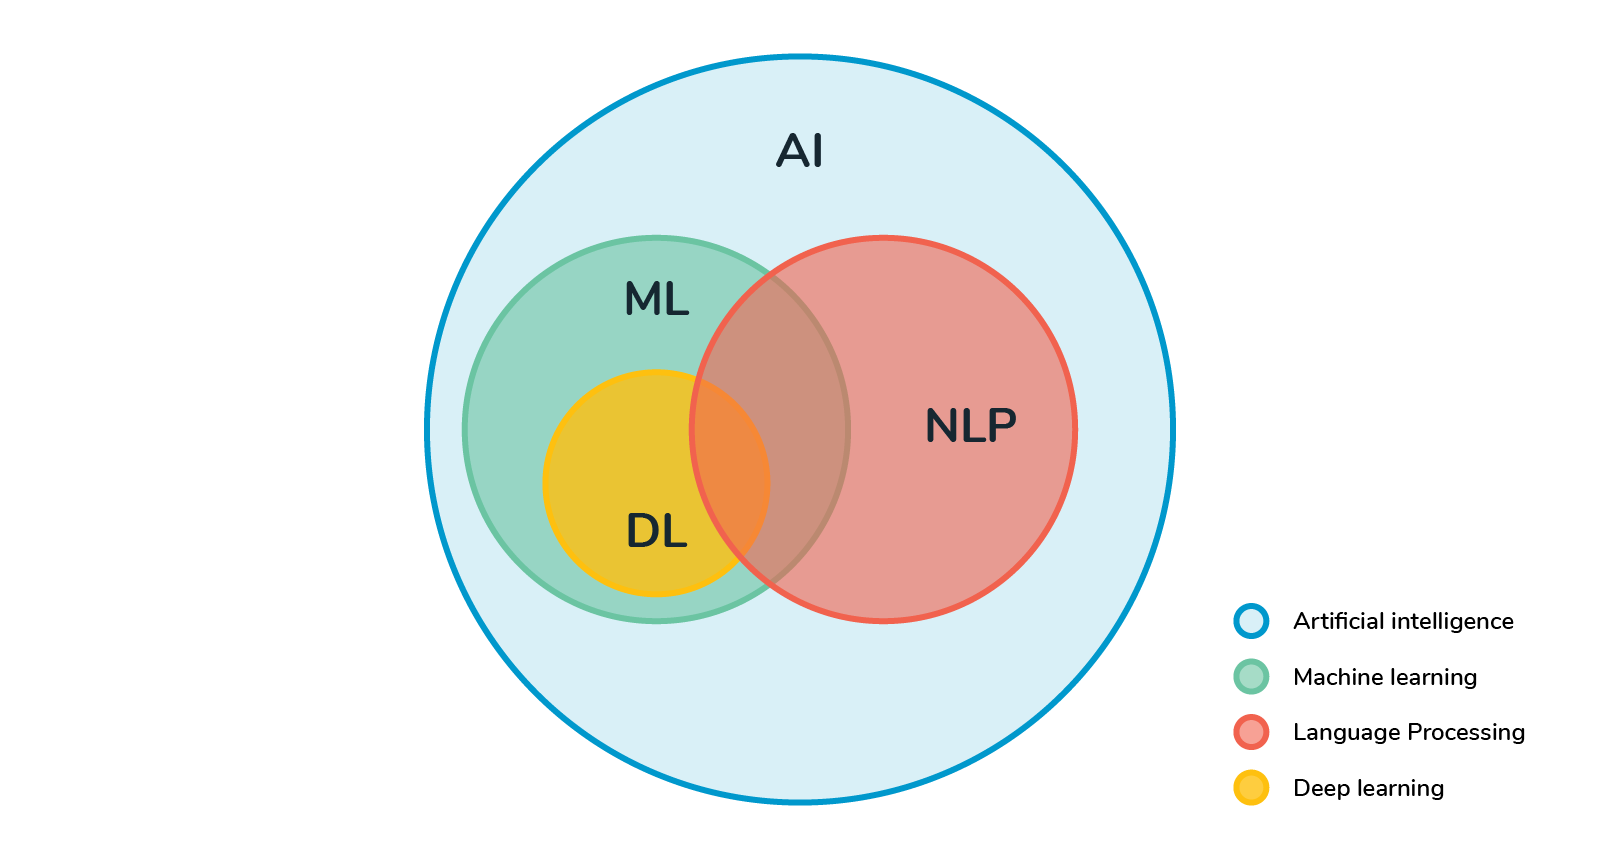
\includegraphics[width=\linewidth]{./assets/images/nln.png}
    \caption{Phương pháp nhúng từ biểu diễn từ thành vector số.}
\end{minipage}
\vspace{0.5cm}


Trong NLP, các mục tiêu chính bao gồm việc phân tích và hiểu ngôn ngữ tự nhiên, dịch máy, tổng hợp tiếng nói, và tạo ra hệ thống trả lời tự động. Điều này đòi hỏi một loạt các kỹ thuật như xử lý ngôn ngữ tự nhiên (NLP) để hiểu ý nghĩa của văn bản, sinh tự động ngôn ngữ tự nhiên (NLP) để tạo ra văn bản tự động, và các phương pháp máy học và học sâu để phân loại, dự đoán và tổng hợp thông tin từ dữ liệu ngôn ngữ.

NLP đang được áp dụng rộng rãi trong nhiều lĩnh vực, từ công nghiệp trí tuệ nhân tạo đến y tế, tài chính, marketing, và giáo dục. Các ứng dụng cụ thể có thể là hệ thống hỏi đáp tự động trên web, phân tích ý kiến công cộng, tổng hợp thông tin từ tài liệu lớn, và dịch máy tự động. Sự phát triển của NLP đã mở ra những cơ hội mới trong việc tạo ra các ứng dụng thông minh có khả năng tương tác với con người một cách tự nhiên và hiệu quả.

\subsubsection{AI tạo sinh - Generative AI}

Một trong những xu hướng của không chỉ \acl{nlp} mà là của lĩnh vực trí tuệ nhân tạo nói chung chính là \textit{Generative AI}

\vspace{0.5cm}
\begin{minipage}{\linewidth}
    \captionsetup{type=figure}
    \centering
    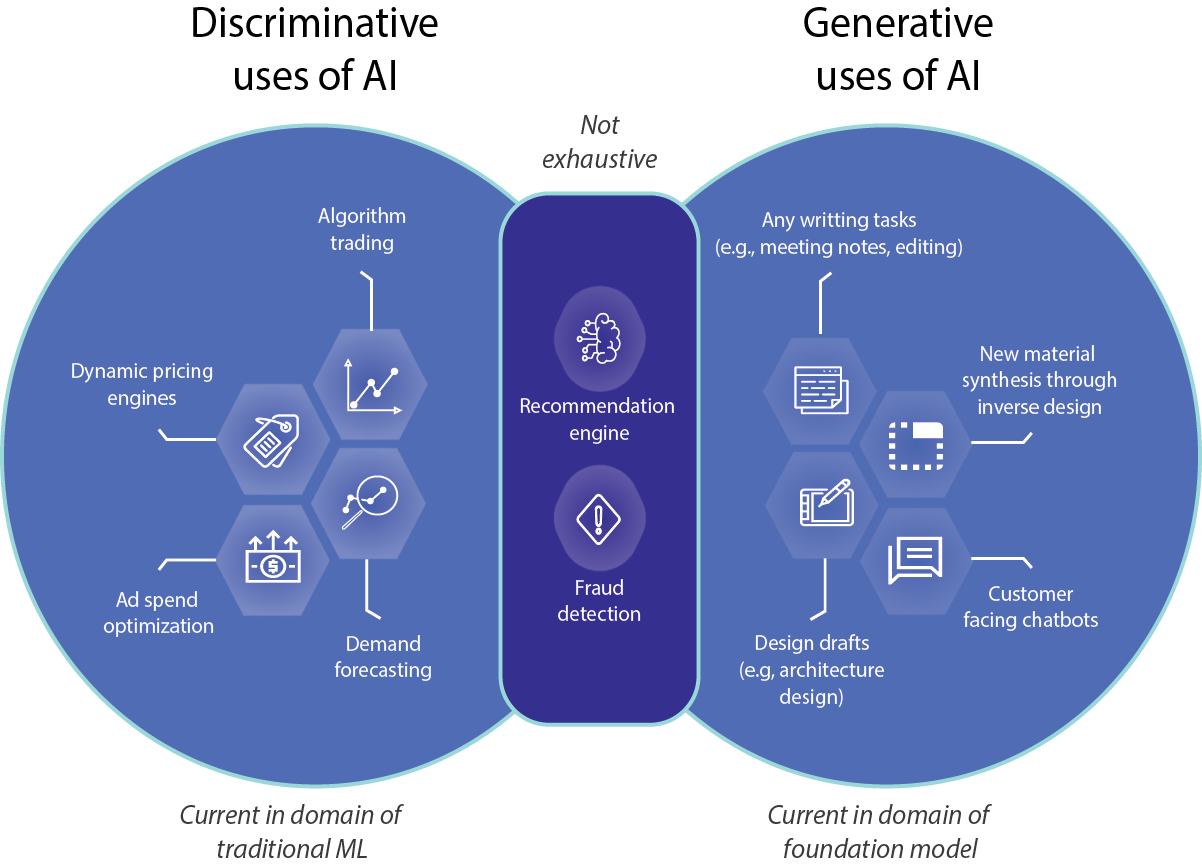
\includegraphics[width=\linewidth]{./assets/images/generative-ai-benefits.png}
    \caption{Generative AI và các ứng dụng của nó.}
\end{minipage}
\vspace{0.5cm}

Generative AI là một lĩnh vực của trí tuệ nhân tạo (AI) tập trung vào việc tạo ra dữ liệu mới, như hình ảnh, văn bản, âm nhạc, và nhiều loại dữ liệu khác, có thể là tự nhiên và chân thực như có thể. Một trong những công cụ phổ biến được sử dụng trong generative AI là Mô hình Ngôn ngữ Dạng Lớn (LLM), như GPT (Generative Pre-trained Transformer).

\acl{llm} là một loại mô hình học sâu (deep learning) dựa trên kiến trúc Transformer, được đào tạo trên một lượng lớn dữ liệu văn bản từ Internet. Đặc điểm nổi bật của LLM là khả năng sinh ra văn bản tự nhiên và có ý nghĩa dựa trên ngữ cảnh. Một số ứng dụng của LLM bao gồm tạo ra văn bản, tổng hợp thông tin, dịch máy, và trả lời câu hỏi.

\subsection{Phương pháp nhúng từ và văn bản}

Các mô hình máy học chỉ có thể hiểu từ vựng của con người dưới dạng số. Từ đó, yêu cầu một phương pháp có thể
ánh xạ từ vựng của con người thành dạng số. Phương pháp nhúng từ (word embedding)
được sinh ra để giải quyết tác vụ này.

\begin{minipage}{\linewidth}
    \captionsetup{type=figure}
    \centering
    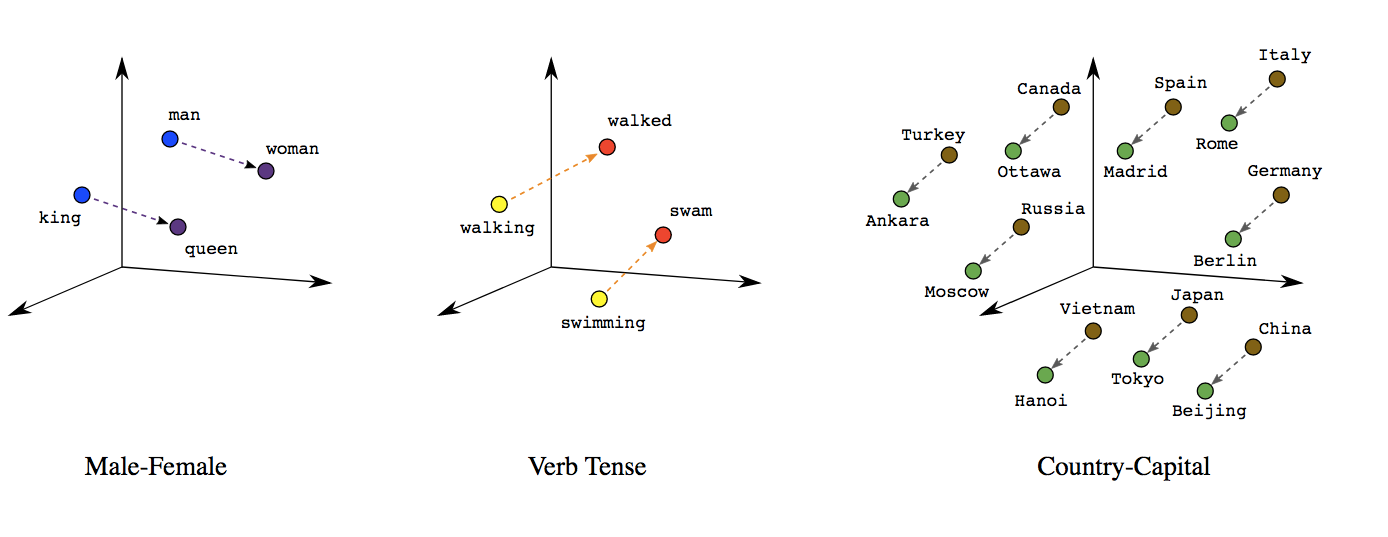
\includegraphics[width=\linewidth]{./assets/images/word_embedding.png}
    \caption{Phương pháp nhúng từ biểu diễn từ thành vector số.}
\end{minipage}
\vspace{0.5cm}

Nhúng từ hay Word Embedding là tác vụ thực hiện ánh xạ các từ hoặc cụm từ sang dạng vector
số (thường là số thực). Các vector từ được biểu diễn theo phương pháp nhúng từ thể hiện
được ngữ nghĩa của các từ, từ đó nhận ra được mối quan hệ giữa các từ với nhau. Nhúng
từ được chia thành 02 loại:


\begin{itemize}
    \item \textbf{Frequency-based embedding}: dựa vào tần suất xuất hiện của các từ để tạo ra các
    vector số đại diện cho từ. Tiêu biểu ở đây sẽ là TF-IDF, Bm25. Mục tiêu của các phương pháp này là
    dựa vào thống kê và xác xuất xuất hiện của từ trong tập từ điển (corpus) để nhúng nghĩa của từ.

    \item \textbf{Prediction-based embedding}: dựa vào mô hình dự đoán từ tiếp theo để tạo ra các
    vector số đại diện cho từ. Tiêu biểu ở đây sẽ là Word2Vec, GloVe, FastText. Mục tiêu của những
    phương pháp này là biểu diễn ngữ nghĩa của từ dưới dạng vector sao cho 
    các từ có ngữ nghĩa tương tự sẽ có vector biểu diễn có khoảng cách gần nhau. Đây là phương pháp
    thường được sử dụng hơn trong các mô hình \ac{nlp} hiện đại.
\end{itemize}

\subsubsection{One hot encoding}
Phương pháp One hot encoding là phương pháp đơn giản nhất để biểu diễn từ dưới dạng vector có độ dài bằng với số từ trong từ điển.
Kỹ thuật này chuyển đổi một từ thành một vector đặc trưng có độ
dài bằng với số lượng từ trong từ điển và chỉ có một giá trị bằng 1 tại vị trí tương ứng với
từ đó, còn lại là giá trị 0.

\begin{minipage}{\linewidth}
    \captionsetup{type=figure}
    \centering
    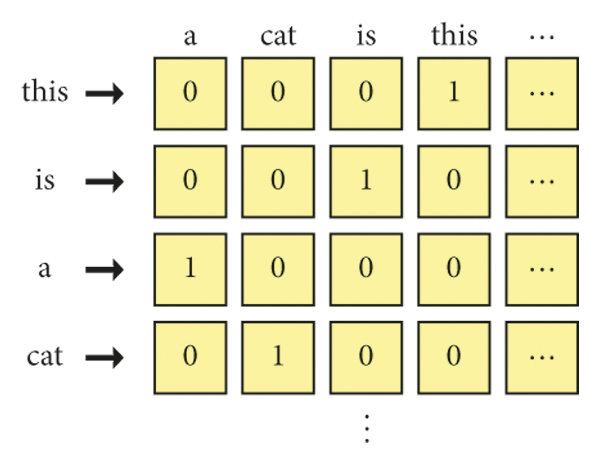
\includegraphics[width=\linewidth]{./assets/images/onehot.png}
    \caption{Phương pháp one hot encoding.}
\end{minipage}
\vspace{0.5cm}

Tuy phương pháp này đã giải quyết được vấn đề biểu diễn từ vựng trong corpus thành 
vector số. Nó vẫn còn rất đơn giản và có nhiều hạn chế như sau:

\begin{itemize}
    \item \textbf{Kích thước vector lớn:} Kích thước của vector biểu diễn từ sẽ phụ thuộc vào số lượng từ trong từ điển. Điều này dẫn đến việc tăng kích thước của vector đầu ra đặc biệt với tập từ điển lớn, làm tăng độ phức tạp của mô hình.
    \item \textbf{Không biểu diễn được ngữ cảnh:} Phương pháp one hot encoding không biểu diễn được ngữ cảnh của từ trong câu. Mỗi từ sẽ được biểu diễn một cách độc lập với các từ khác.
    Nói cách khác, tất cả các từ đều có cùng một khoảng cách với nhau trong không gian vector và không thể giữ được mối quan hệ giữa các từ.
\end{itemize}

\subsubsection{Word2Vec}
Word embedding là một kỹ thuật trong lĩnh vực xử lý ngôn ngữ tự nhiên (NLP) được sử dụng để biểu diễn từ vựng dưới dạng các vector trong không gian nhiều chiều. Ý tưởng cơ bản của word embedding là ánh xạ mỗi từ trong từ điển sang một vector số học, sao cho các từ có ý nghĩa tương tự hoặc thường xuất hiện cùng nhau trong văn bản sẽ có biểu diễn gần nhau trong không gian vector.

\begin{minipage}{\linewidth}
    \captionsetup{type=figure}
    \centering
    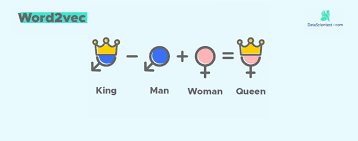
\includegraphics[width=.8\linewidth]{./assets/images/word2vec-intro.png}
    \caption{Một ví dụ về nhúng từ bằng Word2Vec.}
\end{minipage}
\vspace{0.5cm}

Một trong những ưu điểm lớn của word embedding là khả năng biểu diễn từ vựng trong một không gian vector có chiều thấp, giúp giảm chi phí tính toán và không gian lưu trữ. Hơn nữa, những vector biểu diễn từ đã được học có thể bao gồm các mối quan hệ ngữ nghĩa và cú pháp, giúp cải thiện hiệu suất của các mô hình NLP trong nhiều tác vụ, như phân loại văn bản, dịch máy và tóm tắt văn bản.

Trong Word2Vec, có hai kiểu mô hình chính là Skip-gram và Continuous Bag of Words (CBOW). Trong đó, Skip-gram tập trung vào việc dự đoán các từ xung quanh một từ cho trước trong một câu, trong khi CBOW dựa vào ngữ cảnh của từ để dự đoán từ đó.

\begin{minipage}{\linewidth}
    \captionsetup{type=figure}
    \centering
    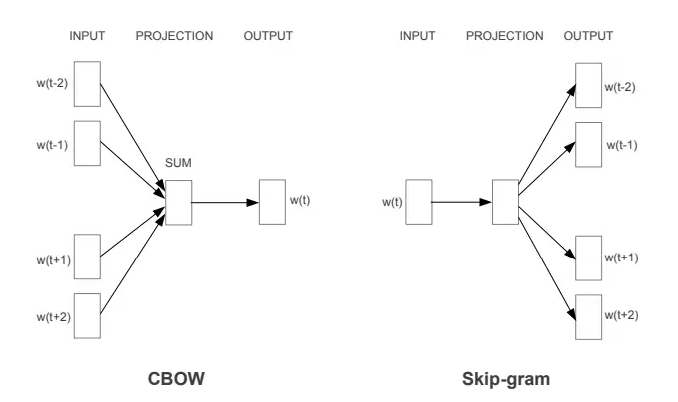
\includegraphics[width=\linewidth]{./assets/images/word2vec.png}
    \caption{Hai kiến trúc cho các mô hình Word2Vec.}
\end{minipage}
\vspace{0.5cm}

\textbf{Huấn luyện và dự đoán mô hình Word2Vec}
Để huấn luyện mô hình Word2Vec, ta sẽ xét một ví dụ sử dụng kiến trúc CBOW.
Đầu tiên, tất cả các từ trong tập dữ liệu sẽ được mã hóa thành dạng one-hot vector. Sau đó, một tầng ẩn sẽ được tạo ra với số lượng nơ-ron bằng với số chiều của vector nhúng. Tầng ẩn này sẽ nhận đầu vào là one-hot vector của từ hiện tại và dự đoán từ tiếp theo trong câu.

\begin{minipage}{\linewidth}
    \captionsetup{type=figure}
    \centering
    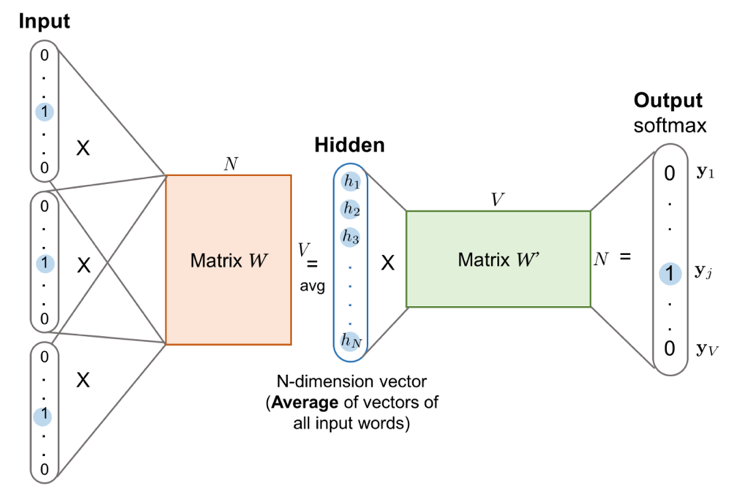
\includegraphics[width=\linewidth]{./assets/images/cbow.png}
    \caption{Huấn luyện mô hình Word2Vec với kiến trúc CBOW.}
\end{minipage}
\vspace{0.5cm}

Ta sẽ áp dụng cửa sổ trượt (sliding window) với một số lượng từ xác định cho mỗi window. Sau đó, từ ở giữa sẽ được dùng để làm nhãn \(\hat{y}\)
các từ còn lại sẽ được dùng làm đầu vào để dự doán cho từ ở giữa đó. Ta lấy ví dụ với câu \textit{"Tôi là sinh viên trường."} với window size = 5:

\begin{itemize}
    \item \textbf{Input}: \textit{"Tôi", "là", "viên", "trường"}
    \item \textbf{Output}: \textit{"sinh"}
\end{itemize}

Mô hình lúc này sẽ nhận các one hot vector của các từ \textit{"Tôi", "là", "viên", "trường"} và dự đoán ra một vector kết quả.
Vector kết quả này sẽ được so sánh với one hot vector của từ \textit{"sinh"} để tính toán lỗi. 
Lỗi này sẽ được lan truyền ngược để cập nhật trọng số của mô hình sao cho lỗi được giảm thiểu.

Kết quả cuối cùng sau khi huấn luyện, ta sẽ có được  một ma trận nhúng từ (embedding matrix) với số hàng bằng với số từ trong từ điển và số cột bằng với số chiều của vector nhúng.
Chọn kích thước embedding vector là 5 cho dữ liệu huấn luyện trên, ta có ma trận trọng số mẫu như sau:

\begin{table}[H]
    \centering
    \begin{tabular}{|c|c|c|c|c|}
        \hline
        w01 & w02 & w03 & w04 & w05 \\ \hline
        w11 & w12 & w13 & w14 & w15 \\ \hline
        w21 & w22 & w23 & w24 & w25 \\ \hline
        w31 & w32 & w33 & w34 & w35 \\ \hline
        w41 & w42 & w43 & w44 & w45 \\ \hline
    \end{tabular}
    \caption{Bảng ma trận nhúng từ sau khi huấn luyện với Word2Vec.}
\end{table}

Khi muốn sử dụng mô hình đã huấn luyện để nhúng từ mới, ta sẽ nhân từ mới với ma trận nhúng từ để lấy vector nhúng của từ đó:

\begin{equation}
    \text{Embedding vector của từ mới} = \text{One hot vector của từ mới} \times W
\end{equation}

Cách huấn luyện cũng gần tương tự với kiến trúc Skip-gram, tuy nhiên kiến trúc này sẽ dự đoán các từ xung quanh từ hiện tại:

\vspace{0.5cm}
\begin{minipage}{\linewidth}
    \captionsetup{type=figure}
    \centering
    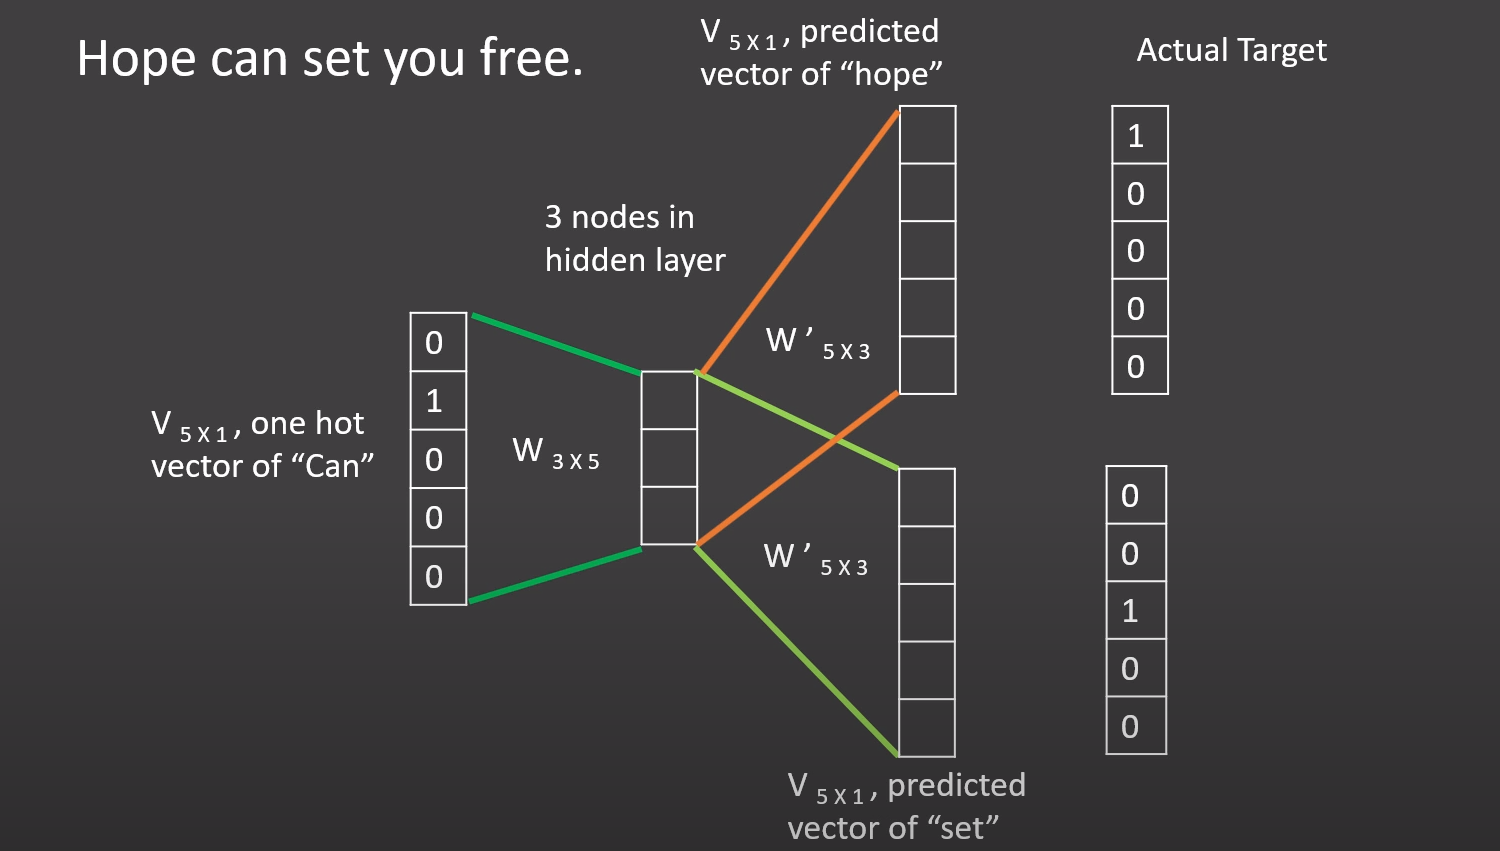
\includegraphics[width=\linewidth]{./assets/images/skipgram.png}
    \caption{Huấn luyện mô hình Word2Vec với kiến trúc Skip-gram.}
\end{minipage}
\vspace{0.5cm}

\subsubsection{Nhúng từ bằng phương pháp Tf-Idf}


TF-IDF (Term Frequency-Inverse Document Frequency) là một kỹ thuật quan trọng trong xử lý ngôn ngữ tự nhiên được sử dụng để đánh giá sự quan trọng của một từ trong một tài liệu so với một tập hợp các tài liệu khác. Kỹ thuật này kết hợp giữa tần số xuất hiện của từ trong một tài liệu (TF) và tần suất nghịch đảo của từ đó trong tất cả các tài liệu (IDF).

\begin{minipage}{\linewidth}
    \captionsetup{type=figure}
    \centering
    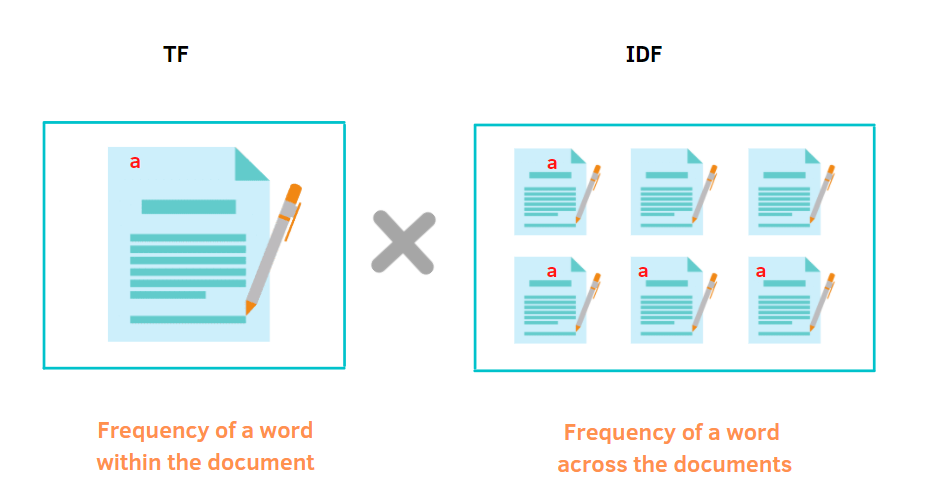
\includegraphics[width=\linewidth]{./assets/images/tf-idf.png}
    \caption{Phương pháp Tf-Idf.}
\end{minipage}
\vspace{0.5cm}

\begin{itemize}
    \item Tần số xuất hiện của từ (TF): Đo lường tần suất xuất hiện của một từ trong một tài liệu cụ thể. TF tăng khi tần suất xuất hiện của từ trong tài liệu càng cao. Ta có thể tính TF theo công thức:
    \begin{center}
        \(TF(t, d) = \frac{\text{Số lần từ t xuất hiện trong tài liệu d}}{\text{Tổng số từ trong tài liệu d}}\)
    \end{center}
    
    \item Tần suất nghịch đảo của từ (IDF): Đo lường độ quan trọng của một từ bằng cách đo tần suất xuất hiện của từ đó trong toàn bộ tập hợp các tài liệu. Các từ phổ biến như "và", "là" thường xuất hiện nhiều trong một số lượng lớn các tài liệu, do đó tần suất nghịch đảo của chúng thấp, trong khi các từ đặc biệt hoặc hiếm có tần suất nghịch đảo cao.
    Ta có thể tính IDF theo công thức:

    \begin{center}
        \(IDF(t, D) = \log\left(\frac{\text{Tổng số tài liệu trong tập D}}{\text{Số tài liệu chứa từ t trong tập D}}\right)\)
    \end{center}
\end{itemize}

Chỉ số TF-IDF cuối cùng của từ sẽ được tính bằng cách nhân TF và IDF của từ đó:

\begin{center}
    \(TF-IDF(t, d, D) = TF(t, d) \times IDF(t, D)\)
\end{center}

Trong tác vụ biểu diễn từ thành dạng vector số, TF-IDF có thể được coi là một kỹ thuật biểu diễn cơ bản, trong đó các từ được biểu diễn dưới dạng các vector của các điểm TF-IDF của chúng qua nhiều tài liệu. Mặc dù đơn giản, TF-IDF có thể hiệu quả trong các nhiệm vụ như truy xuất thông tin và phân loại văn bản.

\subsubsection{Nhúng từ bằng phương pháp Bm25}

Bm25 là một phương pháp đánh giá mức độ quan trọng của một từ trong một tài liệu so với một tập hợp các tài liệu khác. Phương pháp này được sử dụng rộng rãi trong các hệ thống tìm kiếm văn bản để xếp hạng các tài liệu phù hợp với một truy vấn cụ thể.

Phương pháp Bm25 cũng kết hợp giữa tần số xuất hiện của từ trong tài liệu (TF) và tần suất nghịch đảo của từ đó trong tất cả các tài liệu (IDF). Tuy nhiên, Bm25 sử dụng một hàm tính toán khác so với TF-IDF.
Mục tiêu của sự thay đổi này so với Tf-IDF là giúp giảm thiểu ảnh hưởng của các từ phổ biến xuất hiện trong nhiều tài liệu.

Ta có công thức để tính điểm Bm25 của từ t trong tài liệu d so với tập hợp tài liệu D như sau:

\begin{center}
    \(BM25(t, d, D) = \log \left( \frac{N - n(t, D) + 0.5}{n(t, D) + 0.5} \right) \times \frac{f(t, d) \times (k_1 + 1)}{f(t, d) + k_1 \times (1 - b + b \times \frac{|d|}{\text{avgdl}})}\)
\end{center}

Điểm khác biệt quan trọng giữa Bm25 và TF-IDF là ở cách tính tần số xuất hiện của từ trong tài liệu (Term Frequency).
Với TF-IDF, khi tần số xuất hiện của từ tăng, điểm TF-IDF cũng tăng theo. Trong khi đó, với Bm25, điểm Bm25 sẽ tăng khi tần số xuất hiện của từ tăng, nhưng sẽ giảm dần khi tần số xuất hiện của từ tăng quá nhiều.

\begin{minipage}{\linewidth}
    \captionsetup{type=figure}
    \centering
    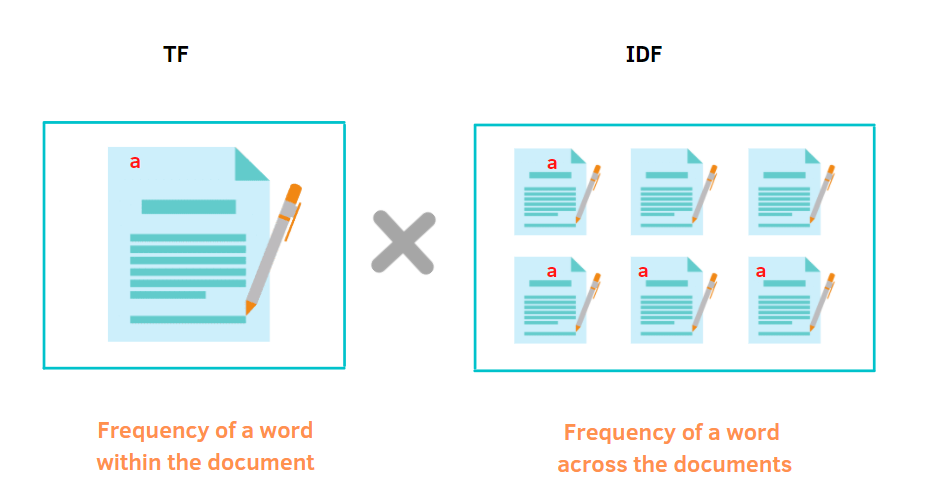
\includegraphics[width=\linewidth]{./assets/images/tf-idf.png}
    \caption{Khác nhau trong giá trị tần suất xuất hiện giữa Bm25 và TF-IDF.}
\end{minipage}

\subsection{Mô hình Seq2Seq và cơ chế attention}
\subsubsection{Mô hình Seq2Seq}


Mô hình \ac{seq2seq} là một kiến trúc mạng nơ-ron sử dụng cho các tác vụ liên quan đến chuỗi, như dịch máy, tổng hợp văn bản, và phản hồi tự động trong hội thoại. Mô hình này bao gồm hai phần chính: một bộ mã hóa (encoder) và một bộ giải mã (decoder).

\begin{minipage}{\linewidth}
    \captionsetup{type=figure}
    \centering
    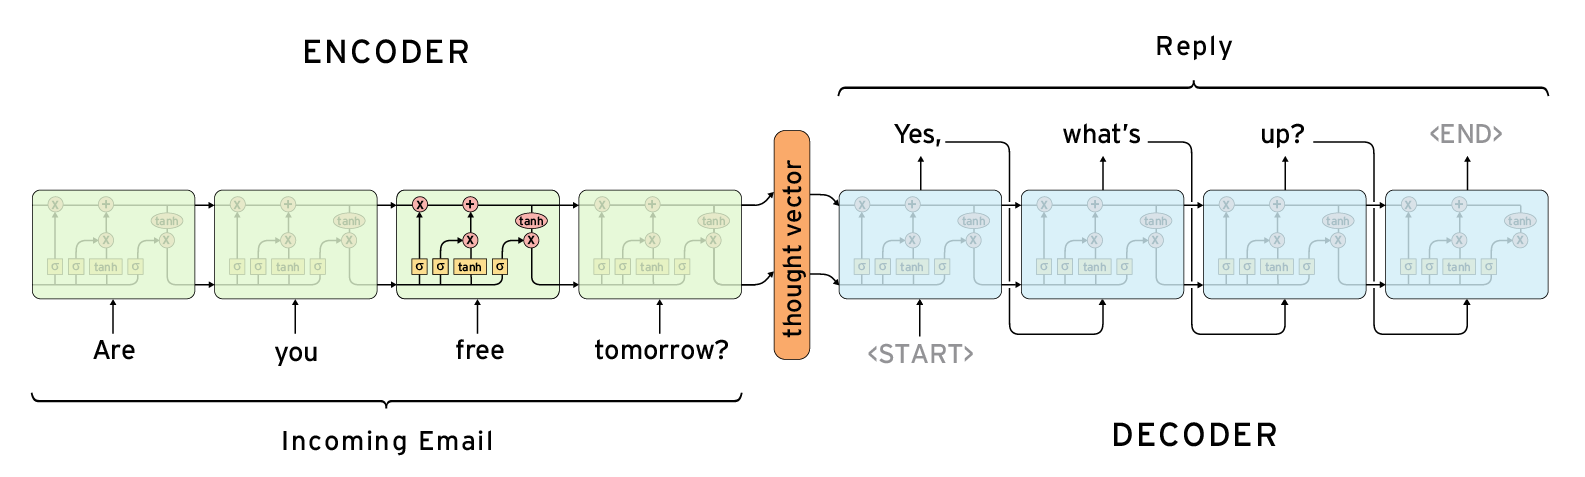
\includegraphics[width=\linewidth]{./assets/images/seq2seq.png}
    \caption{Kiến trúc Seq2Seq trong bài toán hỏi đáp.\cite{sutskever2014sequence}}
\end{minipage}

\vspace{0.5cm}

Mô hình Seq2Seq chính là tập hợp các mô hình \ac{rnn} hoặc các mô hình \ac{gru} được áp dụng vào trong kiến trúc Encoder - Decoder. Mô hình Seq2Seq 
là một công cụ mạnh mẽ cho xử lý và tạo ra các chuỗi, với khả năng thích ứng với nhiều loại dữ liệu và tác vụ khác nhau trong lĩnh vực xử lý ngôn ngữ tự nhiên và trí tuệ nhân tạo.

\begin{minipage}{\linewidth}
    \captionsetup{type=figure}
    \centering
    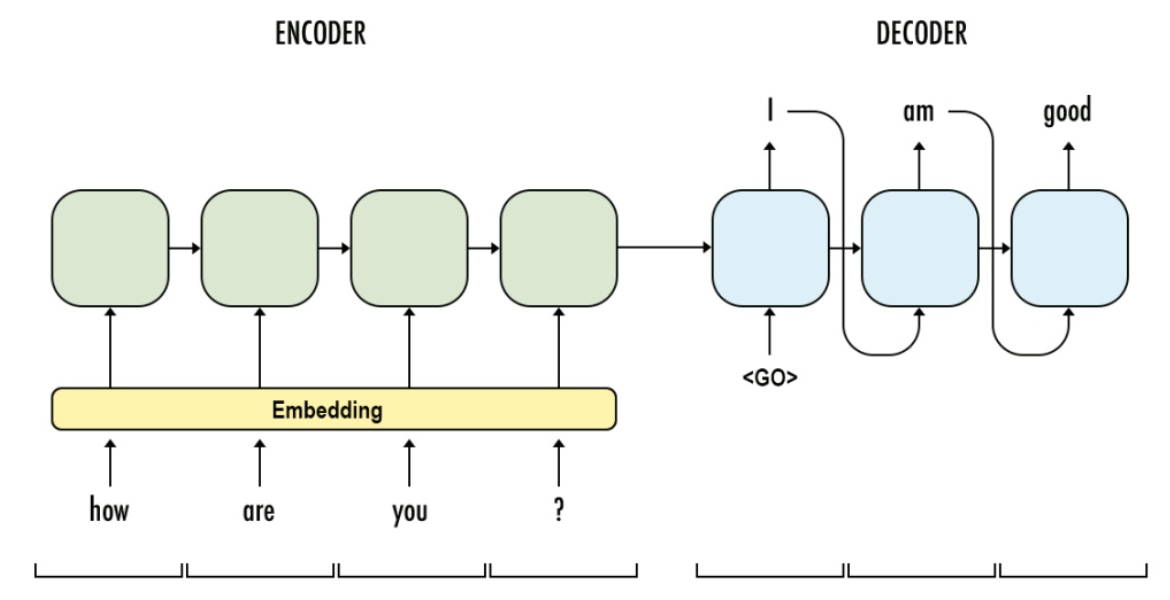
\includegraphics[width=\linewidth]{./assets/images/seq2seq2.png}
    \caption{Chi tiết Kiến trúc Seq2Seq trong bài toán hỏi đáp.\cite{sutskever2014sequence}}
\end{minipage}
\vspace{0.5cm}

Từ hình, ta có thể thấy được đầu vào của \ac{seq2seq} chính là một nhúng từ (embedding) của mỗi từ.
Đầu tiên chúng ta sử dụng
một phương pháp Word Embedding bất kỳ, chẳng hạn như Word2Vec để chuyển
đổi các từ thành vector số thực gọi là Embedding. Sau đó, các Embedding tương ứng với
mỗi từ sẽ được truyền vào Encoder dưới dạng đầu vào.

Mỗi input embedding sẽ được lần lượt được xử lý bởi khối mã hóa (Encoder).
Khối encoder sẽ nén thông tin đầu vào thành một vector ngữ nghĩa (\textbf{context vector}). Encoder sẽ tổng hợp các hidden state của \ac{rnn}:

\begin{center}
    \(h_i = f(W_{hh}h_{i-1} + W_{xh}x_i + b_h)\)
\end{center}

Và vector trạng thái (cell state vectors), được tính theo công thức: 

\begin{center}
    \(c_i = f_c(c_{i-1}, h_{i-1}, x_i) = \sigma(W_{xc}x_i + W_{hc}h_{i-1} + W_{cc}c_{i-1} + b_c)\)
\end{center}


Nói cách khác, mục đích của Encoder chính là tạo ra context vector. Context vector
là một vector đơn giản bao gồm các số thực. Kích thước của context vector có thể được
thiết lập ban đầu khi khởi tạo mô hình, thông thường có thể là 256, 512, 1024.

\begin{minipage}{\linewidth}
    \captionsetup{type=figure}
    \centering
    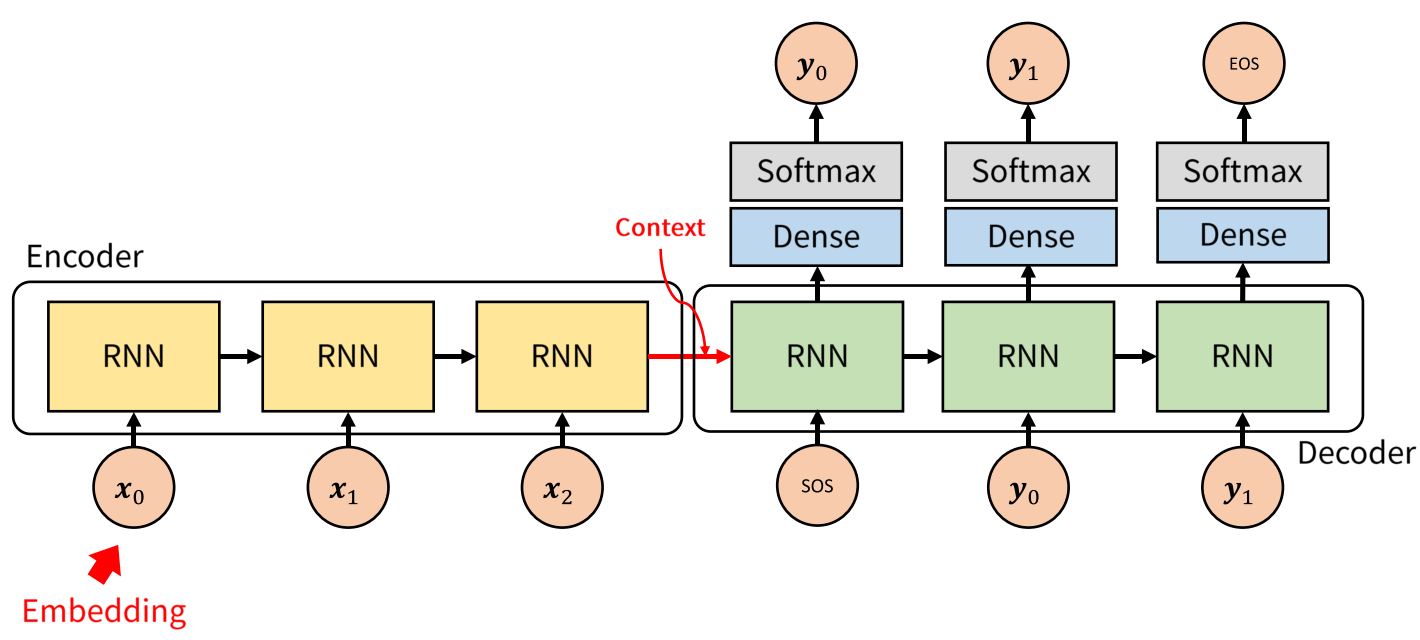
\includegraphics[width=\linewidth]{./assets/images/seq2seq_detail.png}
    \caption{Truyền context vector từ khối Encoder sang Decoder trong \ac{seq2seq}.\cite{sutskever2014sequence}}
\end{minipage}
\vspace{0.5cm}

Context vector lúc này sẽ được khởi tạo và truyền vào khối giải mã (Decoder).
Đơn vị recurrent đầu tiên của khối \textbf{Decoder} sẽ nhận hidden state cuối cùng của Encoder làm hidden state đầu vào.
Tương tự với vector trạng thái:

\begin{center}
    \text{n encoder: số lượng đơn vị recurrent của encoder}

    \(h_0 = h_{\text{n encoder}}\)

    \(c_0 = c_{\text{n encoder}}\)
\end{center}

Token input đầu tiên của Decoder sẽ là token đặc biệt \textbf{<SOS>} (Start of Sentence) để bắt đầu quá trình giải mã (decode) của mô hình.
Kết quả đầu ra \(y_i\) của mỗi đơn vị recurrent sẽ được đưa vào làm đầu vào của đơn vị recurrent tiếp theo cùng với hidden state \(h_i\) và vector trạng thái \(c_i\).
Và kết quả đầu ra này của mỗi đơn vị sẽ được đưa vào một tầng Dense và Softmax để dự đoán từ tiếp theo trong chuỗi.

Điều này sẽ được lặp lại cho đến khi mô hình dự đoán token đặc biệt \textbf{<EOS>} (End of Sentence) hoặc đạt đến giới hạn số từ tối đa cho phép.

\subsubsection{Hạn chế của mô hình Seq2Seq truyền thống}

Với các mô hình \acl{seq2seq} truyền thống, mặc dù khả năng ứng dụng trong nhiều bài toán của Xử Lý Ngôn Ngữ Tự Nhiên (NLP), khi sử dụng sẽ gặp phải các hạn chế như sau:

\begin{itemize}
    \item \textbf{Tốc độ huấn luyện và dự đoán chậm:} Mô hình \ac{seq2seq} truyền thống sử dụng kiến trúc \ac{rnn} hoặc \ac{gru} để xử lý chuỗi, điều này khiến cho mô hình trở nên chậm khi huấn luyện và dự đoán.
    Mỗi đầu vào sẽ phải được xử lý tuần tự từng phần, điều này làm tăng thời gian xử lý của mô hình và không thể tận dụng được khả năng tính toán song song của GPU.
    
    \item \textbf{Triệt tiêu đạo hàm}: Vấn đề triệt tiêu đạo hàm (Vanishing Gradient) là vấn đề với mọi mô hình \ac{rnn} và cả
    các mô hình \ac{seq2seq} truyền thống. Với mạng \ac{rnn}, những chuỗi (sequence) càng dài thì mạng sẽ càng sâu
    theo chiều thời gian. Điều này làm dẫn đến vấn đề Gradient Vanishing khi huấn luyện mô hình \ac{seq2seq}.
    Mặc dù các mô hình như LSTM đã cải thiện vấn đề này, Gradient Vanishing vẫn là một thách thức với mô hình truyền thống.

    \begin{minipage}{\linewidth}
        \captionsetup{type=figure}
        \centering
        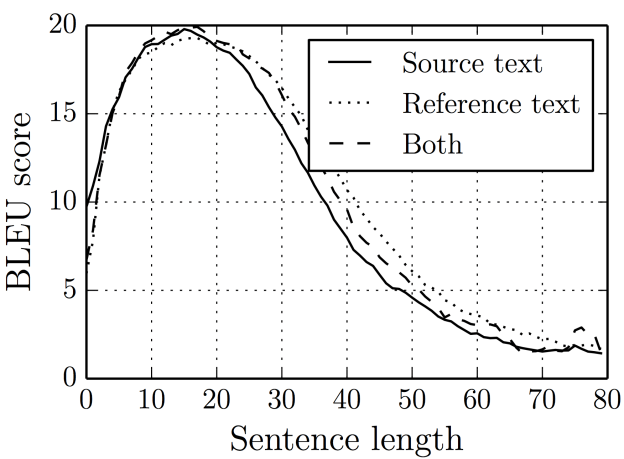
\includegraphics[width=.8\linewidth]{./assets/images/seq2seq_limit.png}
        \caption{Triệt tiêu đạo hàm với số lượng câu dài trong \ac{seq2seq}.}
    \end{minipage}
    \vspace{0.5cm}

    \item \textbf{Mất mát thông tin} Thông tin khi được truyền từ khối mã hóa (Encoder) sang khối giải mã (Decoder)
    chỉ được nén trong một vector ngữ nghĩa (context vector) duy nhất với kích thước cố định.
    Điều này làm cho mô hình \ac{seq2seq} truyền thống không thể hiểu được ngữ cảnh của câu đầu vào một cách tốt và dẫn đến mất mát thông tin.

    \begin{minipage}{\linewidth}
        \captionsetup{type=figure}
        \centering
        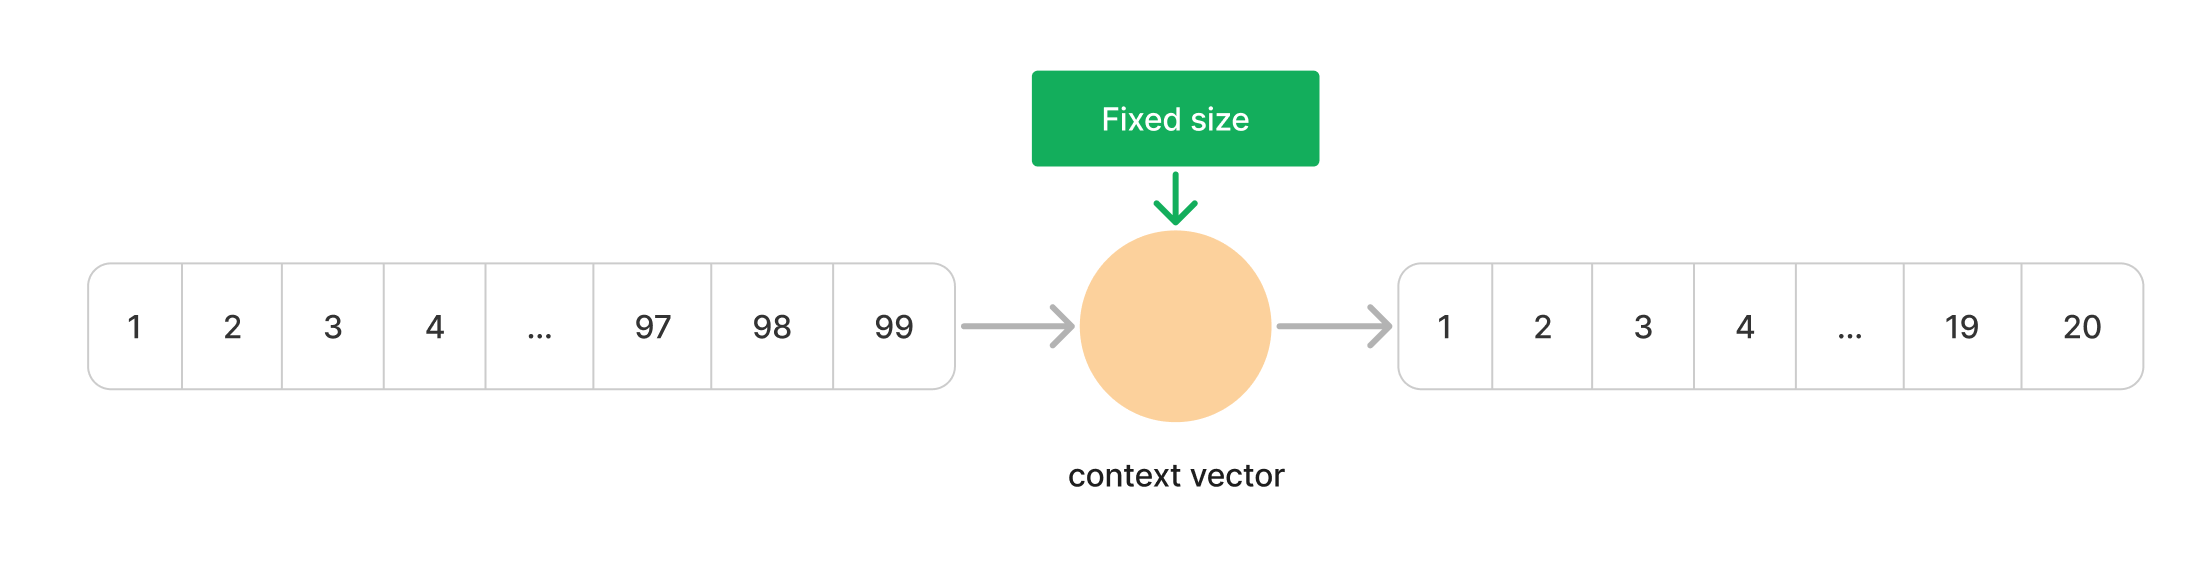
\includegraphics[width=\linewidth]{./assets/images/seq2seq_context_vector.png}
        \caption{Hạn chế khi truyền context vector sang Decoder trong mô hình \ac{seq2seq}.}
    \end{minipage}
    \vspace{0.5cm}

\end{itemize}

\subsubsection{Cơ chế Attention và ứng dụng trong mô hình Seq2Seq}
Để giải quyết các hạn chế của mô hình \ac{seq2seq} truyền thống, ta có thể áp dụng cơ chế tập trung (Attention \cite{vaswani2023attention}) - một cơ chế đã được giới thiệu trong 
bài báo "Attention is All You Need" vào năm 2017 - đánh dấu một bước tiến lớn trong việc xử lý ngôn ngữ tự nhiên và các tác vụ liên quan đến chuỗi.

Áp dụng vào cơ chế Attention vào mô hình \ac{seq2seq}, với mỗi step của Decoder, mô hình sẽ tập trung vào các phần khác nhau của đầu vào (Input) để dự đoán từ tiếp theo trong chuỗi.
Khối Encoder sẽ không truyền hidden state của đơn vị cuối cùng mà sẽ truyền toàn bộ hidden state của mình cho Decoder. 

\begin{minipage}{\linewidth}
    \captionsetup{type=figure}
    \centering
    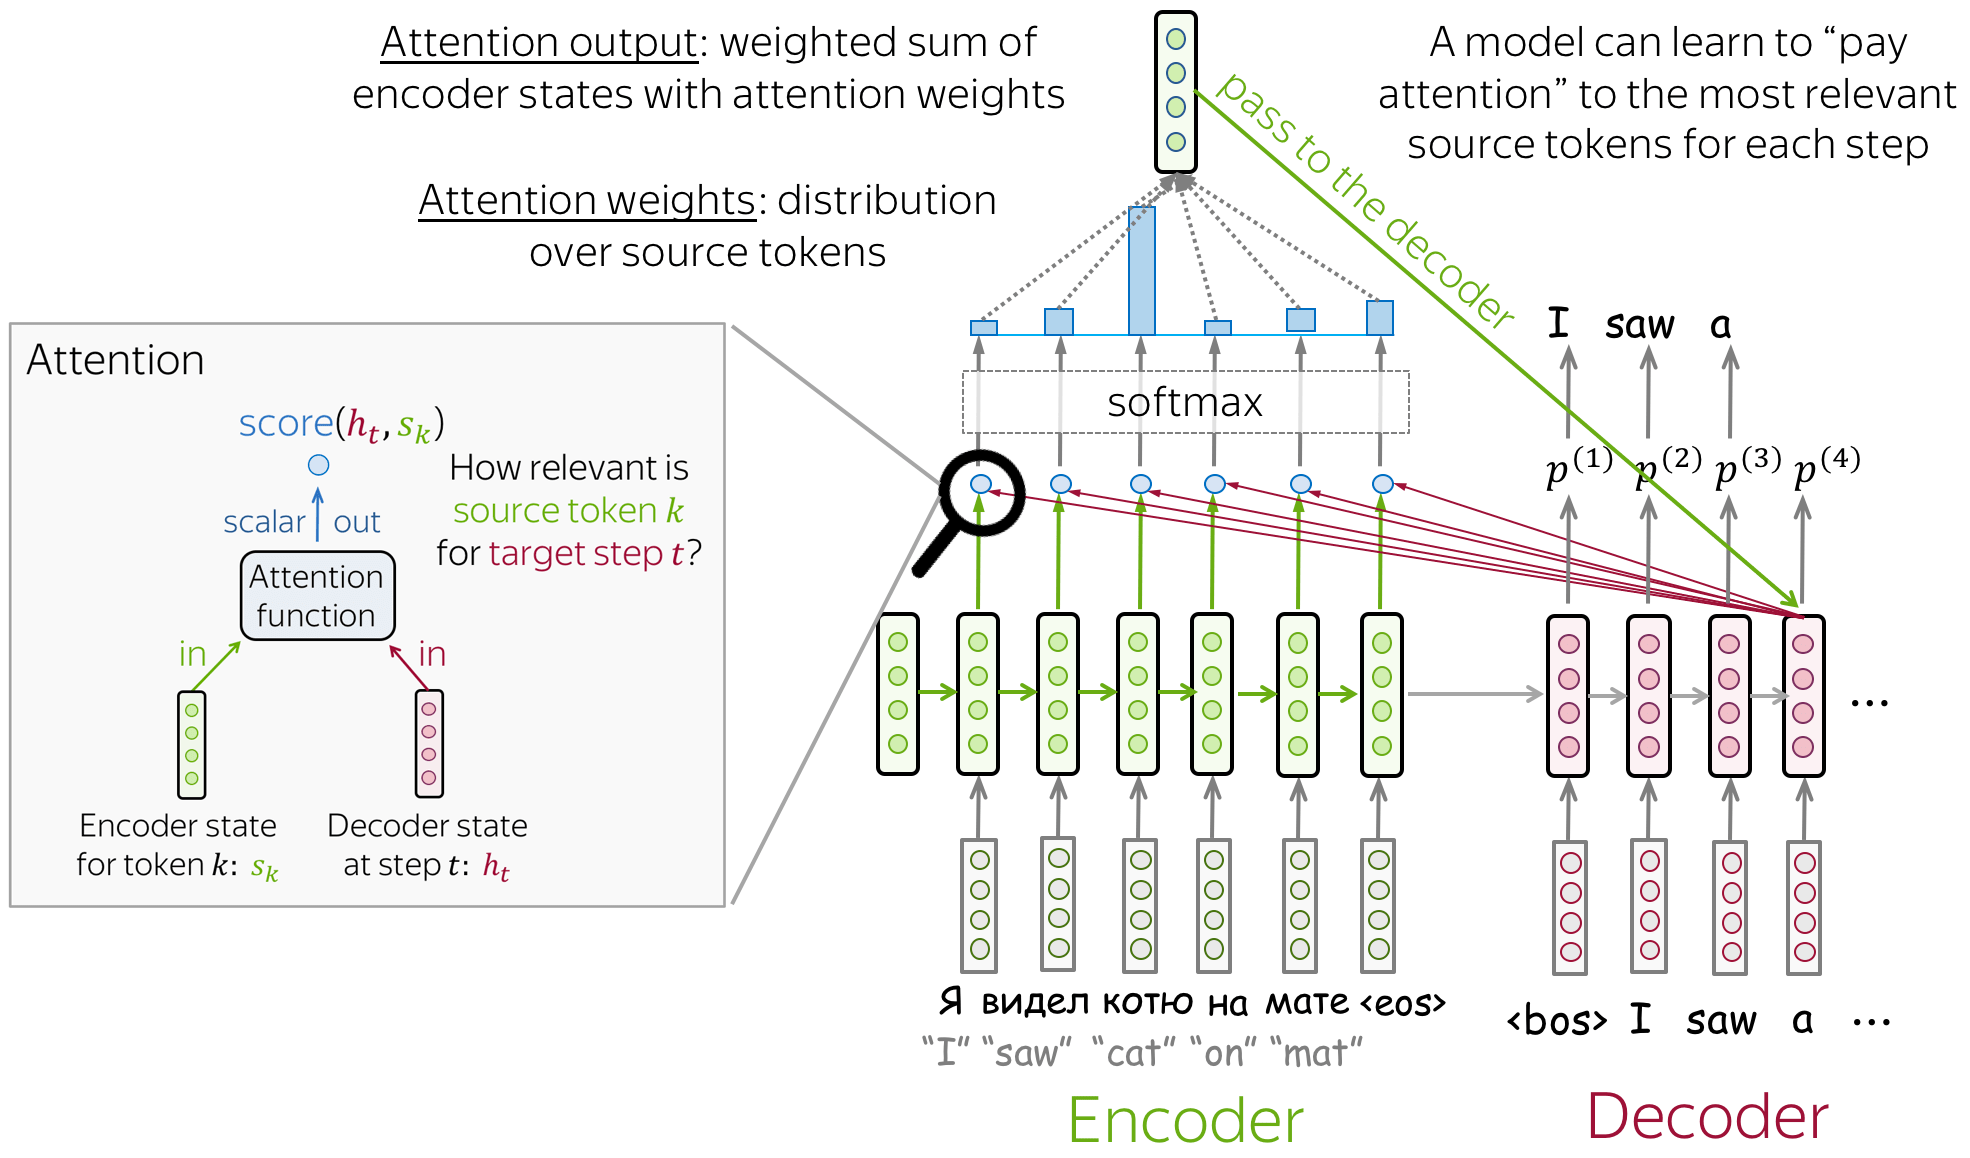
\includegraphics[width=\linewidth]{./assets/images/seq2seq_attention.png}
    \caption{Áp dụng cơ chế Attention trong mô hình \ac{seq2seq}.}
\end{minipage}
\vspace{0.5cm}

Kèm theo đó, trọng số Attention sẽ được tính toán dựa trên hidden state của Encoder và Decoder và 
truyền vào mỗi đơn vị của Decoder để giúp mô hình tập trung vào các phần quan trọng của đầu vào. Ta có sơ đồ tính toán Attention như sau:

\begin{minipage}{\linewidth}
    \captionsetup{type=figure}
    \centering
    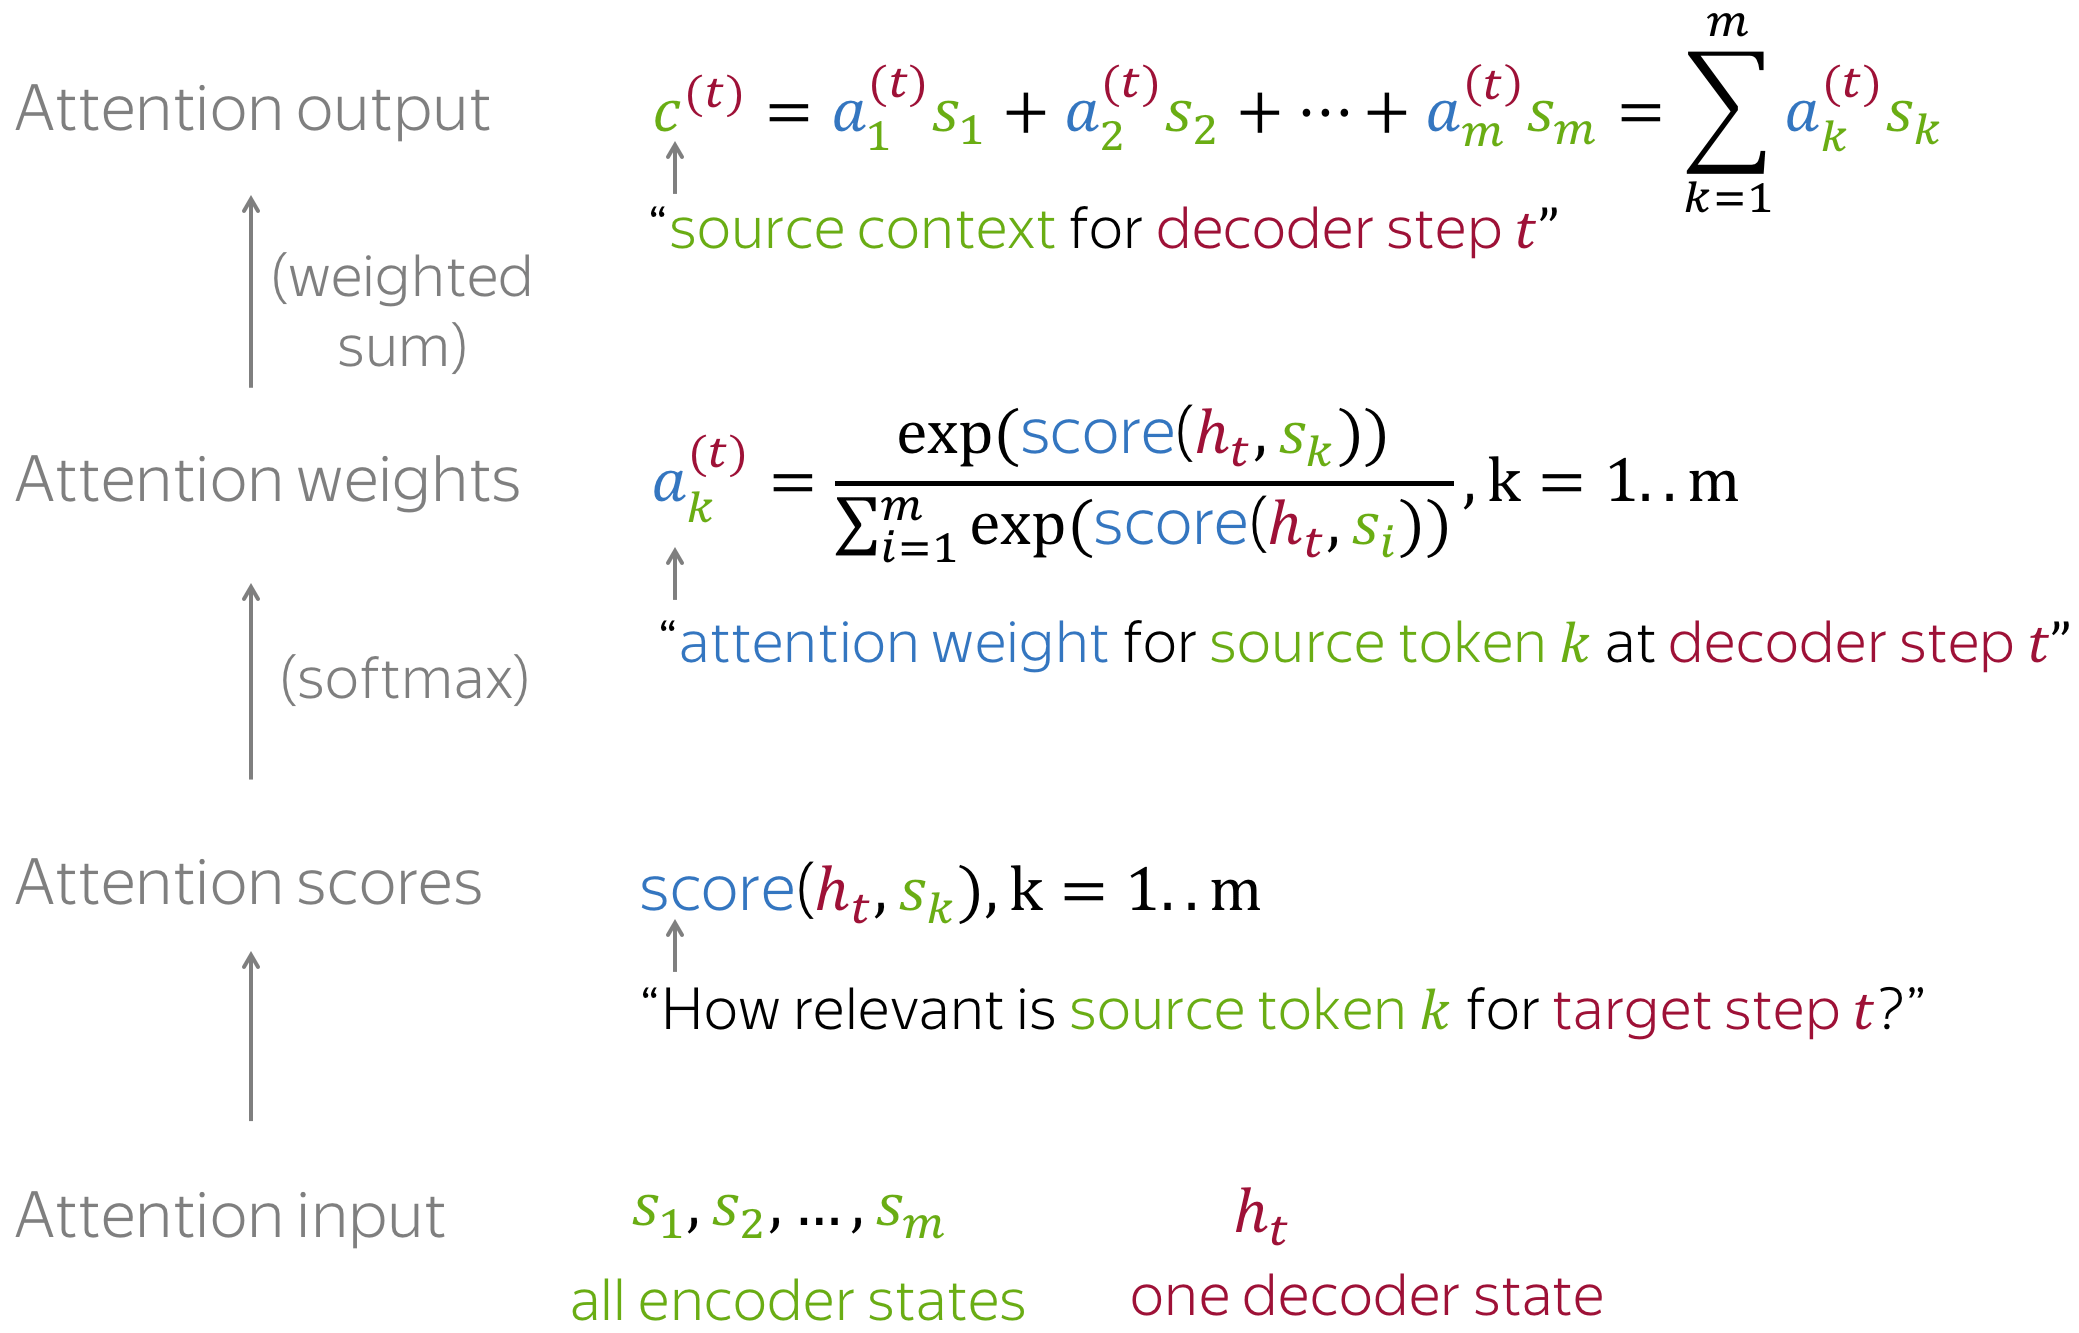
\includegraphics[width=\linewidth]{./assets/images/computation_scheme-min.png}
    \caption{Sơ đồ tính kết quả Attention trong mô hình \ac{seq2seq}.}
\end{minipage}
\vspace{0.5cm}

Đầu vào đầu tiên cho quá trình tính kết quả Attention sẽ là hidden state của Decoder và toàn bộ hidden state của Encoder.
Lúc này, Attention scores sẽ được tính bằng cách áp dụng một hàm Attention Score với m là số đơn vị của khối Encoder:
\begin{center}
    \begin{equation}
        \text{score}(h_t, s_k), k=1,..m
    \end{equation}
\end{center}
\vspace{0.5cm}

Để tính được \( \text{score}(h_t, s_k) \), ta có một số hàm Score Function như sau:

\begin{minipage}{\linewidth}
    \captionsetup{type=figure}
    \centering
    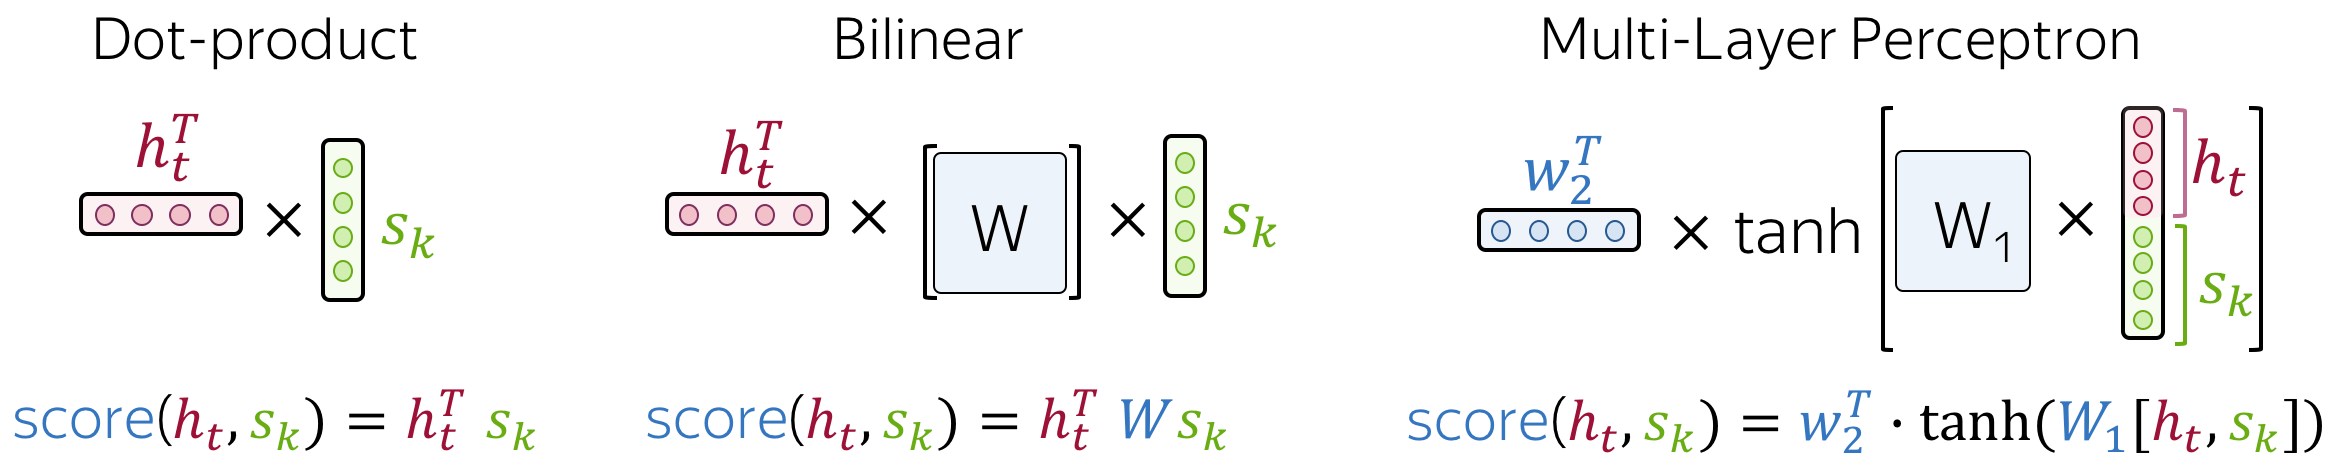
\includegraphics[width=\linewidth]{./assets/images/score_functions-min.png}
    \caption{Một số phương thức tính score cho cơ chế attention.}
\end{minipage}
\vspace{0.5cm}

Sau đó, tiếp tục tính trọng số attention, lúc này ta nhận được một vector trọng số attention cho tất cả m hidden states của Encoder với một hidden state của Decoder:

\begin{equation}
    a_{t,k} = \frac{\exp(\text{{score}}(h_t, s_k))}{\sum_{j=1}^{m} \exp(\text{{score}}(h_t, s_j))}
\end{equation}

Cuối cùng, sau khi đã có được trọng số attention cho step t hiện tại của Decoder, Context Vector tại step t sẽ được tính như sau:

\begin{equation}
    c_t = \sum_{k=1}^{m} a_{t,k} \cdot h_k
\end{equation}


Context vector này sẽ được dùng để làm đầu vào cho đơn vị tại timestep t của khối Decoder để sinh ra từ kế tiếp ở timestep t + 1.

\begin{minipage}{\linewidth}
    \captionsetup{type=figure}
    \centering
    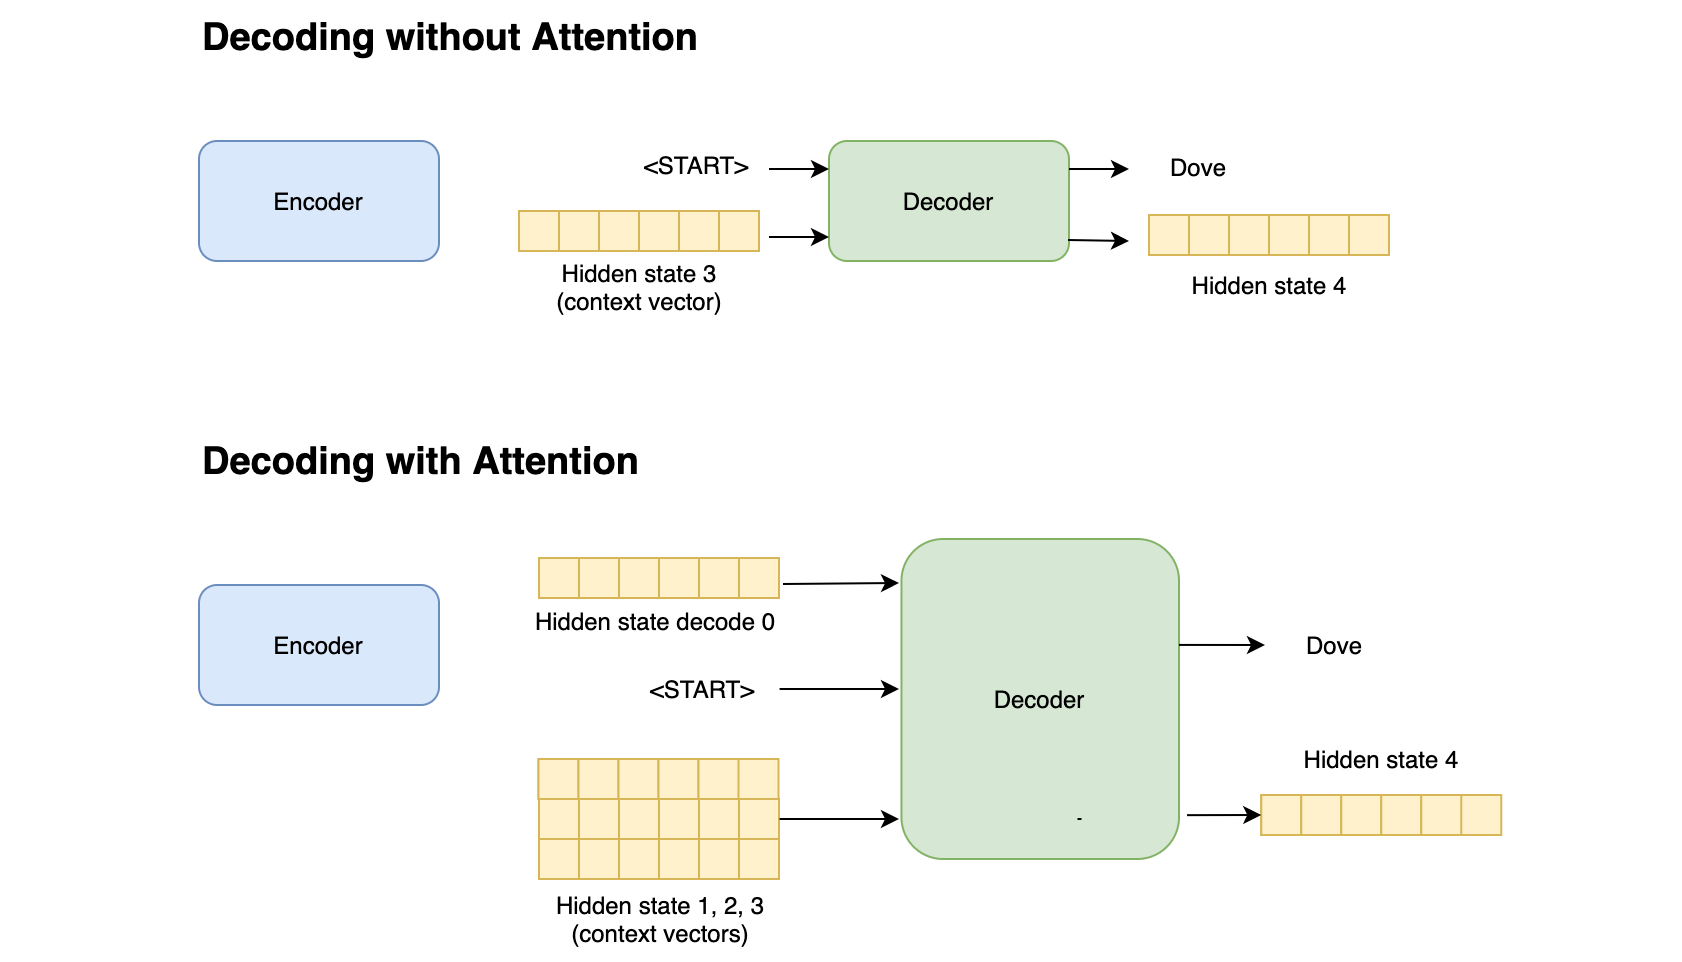
\includegraphics[width=\linewidth]{./assets/images/decoding-attention.png}
    \caption{Khác biệt của khối Decoder khi sử dụng Attention trong mô hình \ac{seq2seq}.}
\end{minipage}
\vspace{0.5cm}

Sự khác biệt ở khối Decoder giữa mô hình \ac{seq2seq} truyền thống và mô hình \ac{seq2seq} áp dụng cơ chế Attention được mô tả như hình trên.
Cụ thể, áp dụng cơ chế attention đã giúp cải thiện việc:

\begin{itemize}
    \item Giữ lại thông tin ngữ nghĩa cho context vector bằng cách tính toán dựa trên toàn bộ hidden states của khối Encoder.
    \item Cho khối Decoder biết thông tin về từ nào nên "tập trung" vào để dự đoán từ tiếp theo. Điều này sẽ hữu ích với dữ liệu có tính cấu trúc (structured bias). Lấy ví dụ như sau: 
    \textit{"Tôi rất thích học môn Toán"}. Ở đây từ "học " và "môn Toán" có mối quan hệ mật thiết với nhau hơn so với các từ khác
\end{itemize}

\subsection{Kiến trúc Transformer}
\subsubsection{Tổng Quan}

Transformer\cite{Wolf2019HuggingFacesTS} là một mô hình học sâu được giới thiệu bởi Vaswani và các cộng sự [9]
vào năm 2017, đây là mô hình đã đạt được kết quả nổi bật trong nhiều nhiệm vụ xử lý
ngôn ngữ tự nhiên (NLP). Transformer được xây dựng dựa trên cơ chế Attention
(Attention mechanism, tạm dịch: cơ chế tập trung), cho phép mô hình có khả năng “tập
trung” vào các phần khác nhau của đầu vào (Input) trong quá trình học.

Mô hình Transformer sử dụng kiến thức đa đầu vào (Multi-Head Input) và đa đầu
ra (Multi-Head Output) để xử lý đầu vào và đầu ra theo cách đồng thời, tức là không cần
xử lý tuần tự từng phần như các mô hình trước đây. Điều này giúp giải quyết vấn đề độ
dài phụ thuộc trong ngôn ngữ (Long-range Dependency) và giúp mô hình có khả năng
hiểu ngữ cảnh (Contextual Understanding) của dữ liệu đầu vào (Input).

Mô hình Transformer đã được ứng dụng rộng rãi trong nhiều tác vụ xử lý ngôn ngữ
tự nhiên, bao gồm dịch máy, phân loại văn bản, dự đoán từ, tóm tắt văn bản, hỏi đáp, và
nhiều tác vụ ngôn ngữ tự nhiên khác. BERT\cite{BERT} (Bidirectional Encoder Representations from
Transformers), GPT\cite{yenduri2023generative} (Generative Pre-trained Transformer), và T5\cite{raffel2023exploring} (Text-to-Text Transfer
Transformer) là những mô hình NLP nổi tiếng được xây dựng trên kiến trúc của mô hình
Transformer.

\begin{minipage}{\linewidth}
    \captionsetup{type=figure}
    \centering
    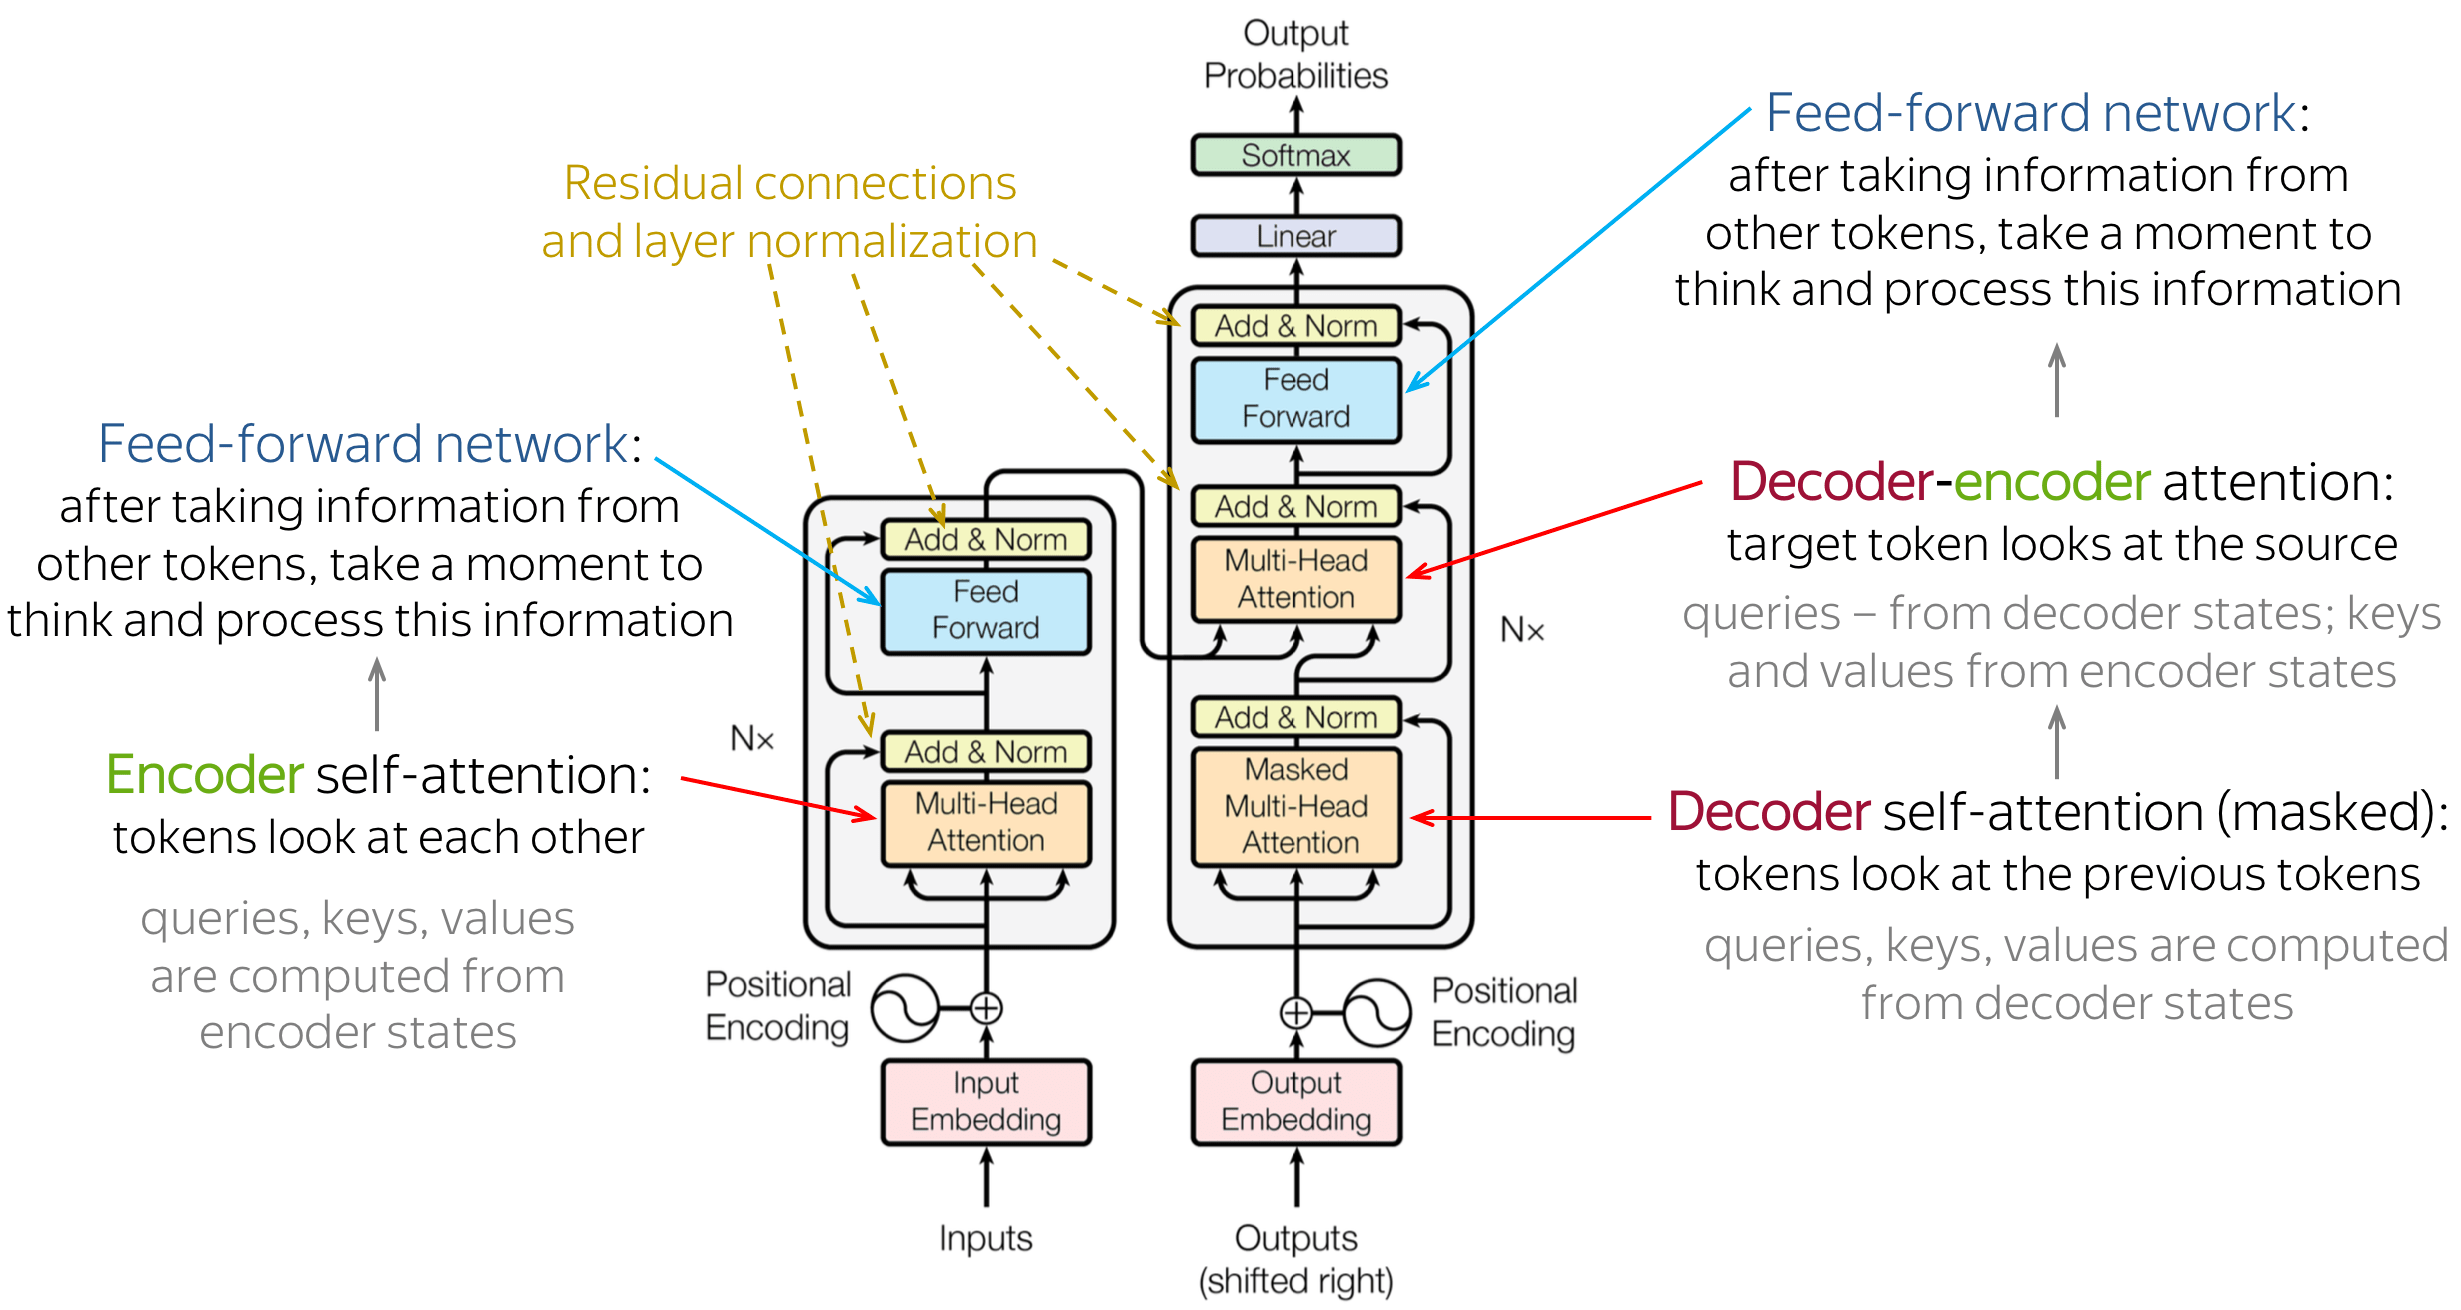
\includegraphics[width=\linewidth]{./assets/images/transformer.png}
    \caption{Tổng quan kiến trúc Transformer\cite{vaswani2023attention}}
\end{minipage}

\begin{itemize}
    \item[--]  Mô hình Transformer sử dụng định dạng mã hóa - giải mã (Encoder - Decoder)
        tương tự như Seq2Seq.
    \item[--]  Những khối được đề xuất trong Transformer, bao gồm Scaled Dot-Product
        Attention và Multi-Head Attention, là trọng tâm của kiến trúc này, và chúng
        được xếp hàng loạt và thực hiện song song (parallel) trong mô hình.
    \item[--] Khác với kiến trúc của RNN,transformer, không có cấu trúc BPTT tương tự và tính toán
        có thể được thực hiện song song, do đó mô hình có khả năng hoạt động hiệu quả
        hơn so với kiến trúc RNN.
\end{itemize}

\subsubsection{Hai khối Encoder và Decoder}
Đầu vào và đầu ra của Encoder có cùng kích thước. Do đó, cấu trúc Encoder có thể
được lặp lại nhiều lần để sử dụng một cách dễ dàng.

Tương tự, Decoder cũng có thể được lặp lại
nhiều lần dưới dạng khối để giải mã đầu ra.

\begin{minipage}{\linewidth}
    \captionsetup{type=figure}
    \centering
    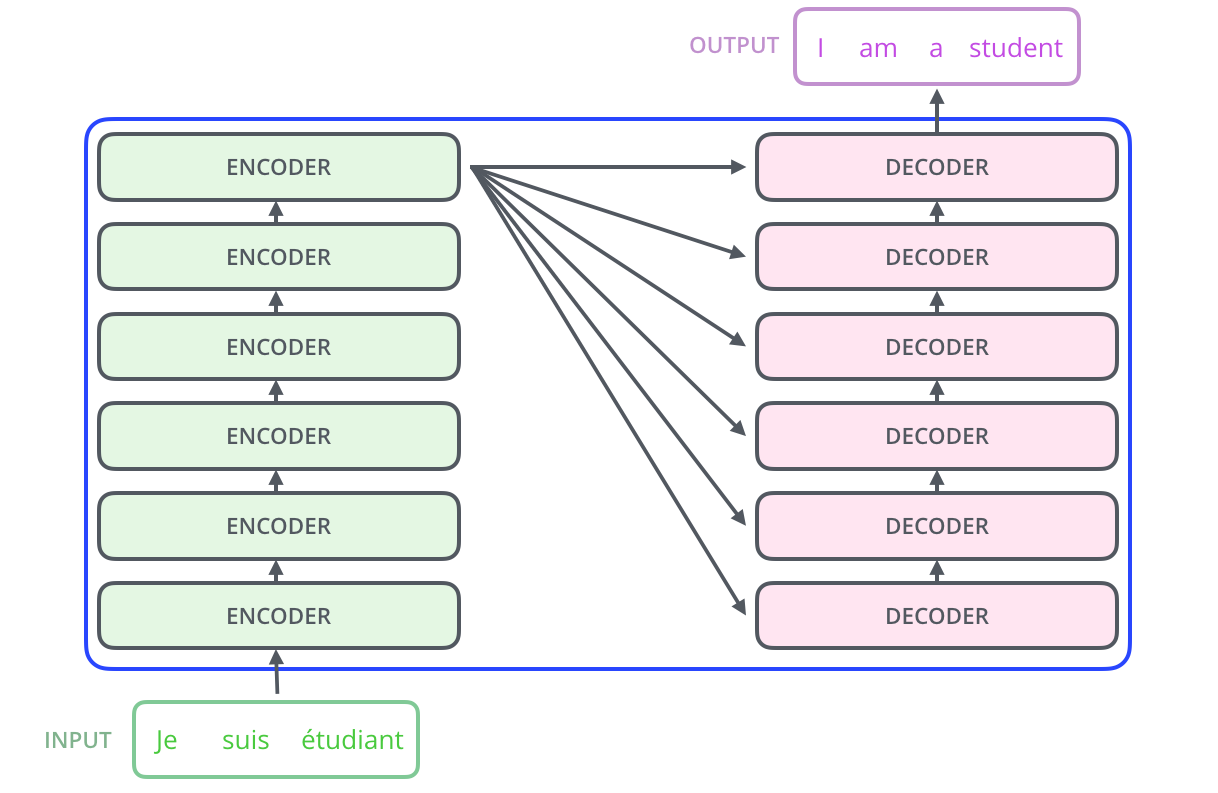
\includegraphics[width=\linewidth]{./assets/images/The_transformer_encoder_decoder_stack.png}
    \caption{Chồng các khối Encoders và Decoders\cite{vaswani2023attention}}
\end{minipage}

\subsubsection{Embedding và Positional Encoding}
\textbf {Input Embedding và Output Embedding}
Trong Transformer, Input Embedding và Output Embedding đều là tầng Embedding
để chuyển đổi đầu vào thành vector với số thực.

Đây là tầng đầu tiên trong kiến trúc Transformer, nhận đầu vào là một
one-hot-encoded vector là một vector có độ dài bằng với số từ trong từ điển,

Mỗi từ đi vào sẽ được tầng này tạo ra một vector đặc, có số chiều nhỏ hơn ban đầu.
\textbf {Positional Encoding}
Kết quả của tầng Input Embedding hoặc Output Embedding
sẽ được đi qua một phép tính Positional Encoding.

\begin{minipage}{\linewidth}
    \captionsetup{type=figure}
    \centering
    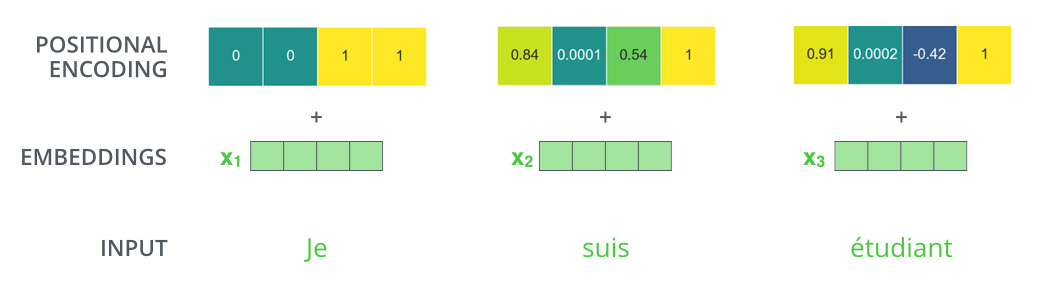
\includegraphics[width=\linewidth]{./assets/images/transformer_input.png}
    \caption{Tầng Input và Output của Transformers\cite{vaswani2023attention}}
\end{minipage}


Do Transformer không tính toán tuần tự mà xử lý một cách song song , nên nó không có khả năng
nhận biết được vị trí của từ trong câu. Mục tiêu của phép tính
Positional Encoding là để giữ lại vị trí cho câu input, không làm mất thứ tự và ngữ nghĩa câu.

\subsubsection{Khối Multi-Headed Attention}
\textbf{Scaled Dot-Product Attention}
Attention là một cơ chế cho phép mô hình tập trung vào những phần quan trọng của đầu vào (Input) trong quá trình học.
Cơ chế Attention được sử dụng trong nhiều mô hình NLP, bao gồm cả mô hình Transformer.

\begin{minipage}{\linewidth}
    \captionsetup{type=figure}
    \centering
    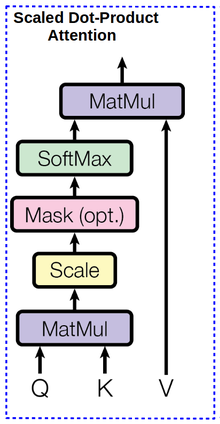
\includegraphics[width=.2\linewidth]{./assets/images/ScaledDotProductAttention.png}
    \caption{Khối ScaleDotProductAttention\cite{vaswani2023attention}}
\end{minipage}

Đầu vào của Scaled Dot-Product Attention là 3 ma trận Q, K, V có cùng số chiều.

Đầu ra của Scaled Dot-Product Attention là ma trận có cùng số hàng với ma trận Q và cùng số cột với ma trận V thể hiện trọng số attention của nó.

Dữ liệu trong khối này sẽ được xử lý như sau: \begin{itemize}
    \item[--] Hai ma trận Q và K sẽ được nhân lại với nhau, sau đó chia cho căn bậc hai của số chiều
        của ma trận K (tầng Scale) nhằm ngăn giá trị tăng lên quá lớn .
    \item[--] Sau tầng Scale, nếu có tầng Mask thì sẽ được thực hiện để ngăn chặn Attention đến các kết nối không
        hợp lệ (illegal connection).
    \item[--] Sau đó, ma trận sau khi được nhân sẽ được đưa vào hàm softmax để chuẩn hóa giá trị Attention. Giúp mô hình tự tin hơn với các trọng số.
    \item[--] Cuối cùng, ma trận sau khi được chuẩn hóa sẽ được nhân với ma trận V để tạo ra đầu ra của khối Scaled Dot-Product Attention. Đây chính là trọng số Attention của khối.
\end{itemize}

\textbf{Multi-headed Attention}

Thay vì chỉ sử dụng một khối Scaled Dot-Product Attention, Transformer sử dụng
nhiều khối Scaled Dot-Product Attention song song (parallel) để tăng khả năng học của mô hình, hiểu ngữ nghĩa theo nhiều khối.

Đầu ra của mỗi khối Scaled Dot-Product Attention sẽ được nối với nhau và đi qua một tầng Linear để tạo ra đầu ra của khối Multi-Headed Attention.

Kết quả của khối là một ma trận có cùng số hàng với ma trận Q và cùng số cột với ma trận V thể hiện trọng số attention của nó.

\begin{minipage}{\linewidth}
    \captionsetup{type=figure}
    \centering
    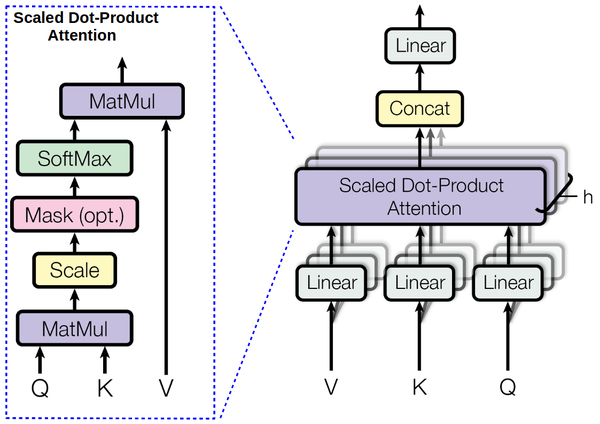
\includegraphics[width=.6\linewidth]{./assets/images/MultiHead.png}
    \caption{Multi-headed Attention\cite{vaswani2023attention}}
\end{minipage}

\subsubsection{Add và LayerNormalization}
Trong Transformer, Add \& Norm được sử dụng để kết hợp thông tin
từ các tầng khác nhau trong mạng. Trong quá trình này, đầu ra của một tầng sẽ được
cộng với đầu vào ban đầu của tầng đó (skip-connection), sau đó chuẩn hóa lại với Layer
Normalization để tạo ra đầu ra cuối cùng.

\begin{minipage}{\linewidth}
    \captionsetup{type=figure}
    \centering
    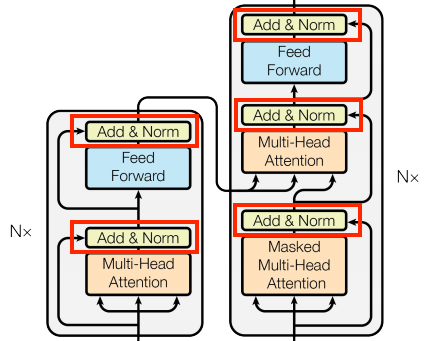
\includegraphics[width=.8\linewidth]{./assets/images/Add+Norm.png}
    \caption{Tầng Add và LayerNormalization\cite{vaswani2023attention}}
\end{minipage}
\textbf{Add}
Trong bước này, đầu ra của lớp sẽ được cộng với vector
đầu vào ban đầu. Việc cộng này giúp cập nhật thông tin từ các phần khác nhau của kiến
trúc và giúp tránh hiện tượng mất thông tin (Vanishing Gradient) trong quá trình huấn
luyện.

\textbf{LayerNormalization}
Sau khi được cộng với đầu vào ban đầu, đầu ra của lớp sẽ được chuẩn hóa lại với
Layer Normalization. Layer Normalization là một phép chuẩn hóa dữ liệu đầu ra của
một tầng theo của ma trận đầu ra. Quá
trình chuẩn hóa giúp cải thiện tính ổn định của mô hình

\subsubsection{Position-wise Feed Forward Network}
\begin{minipage}{\linewidth}
    \captionsetup{type=figure}
    \centering
    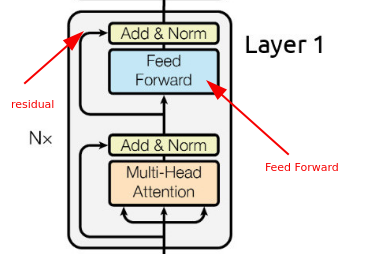
\includegraphics[width=.6\linewidth]{./assets/images/feed-forward-sublayer-in-transformer.png}
    \caption{Khối Position-wise Feed Forward\cite{vaswani2023attention}}
\end{minipage}

Các vector đầu vào (là các vector đại diện cho từ) sẽ được truyền qua tầng Fully Connected Layer với hàm kích hoạt ReLU, và cuối cùng đi qua một tầng Fully ConnectedLayer nữa.
Đầu ra của tầng thứ hai cũng chính ra đầu ra của Position-wise Feed-Forward.

Mục đích chính là xử lý tiếp attention output từ tầng trước đó, giúp mô hình có thể học được các mối quan hệ giữa các từ trong câu.

\subsection{Các mô hình Pretrained}

Pretraining model là quá trình huấn luyện một mạng nơ-ron trên một lượng lớn dữ liệu không được gắn nhãn trước đó, để học các biểu diễn cơ bản của dữ liệu. 
Mục tiêu của pretraining là tạo ra một mô hình mạng nơ-ron có khả năng học được các đặc trưng chung, tổng quát từ dữ liệu lớn, sau đó có thể được fine-tuning hoặc điều chỉnh lại trên một tập dữ liệu cụ thể cho một tác vụ cụ thể. 

Trong quá trình pretraining, mô hình thường được huấn luyện trên một tác vụ phụ, thường là dự đoán từ tiếp theo trong chuỗi dữ liệu (Masked Language Modeling), dựa trên các mô hình ngôn ngữ như BERT (Bidirectional Encoder Representations from Transformers) hoặc GPT (Generative Pre-trained Transformer). 
Sau khi pretraining, mô hình sẽ hiểu được cấu trúc và ngữ cảnh của dữ liệu đầu vào một cách tổng quát, giúp nó học được các biểu diễn sâu và phức tạp của dữ liệu.

\begin{minipage}{\linewidth}
    \captionsetup{type=figure}
    \centering
    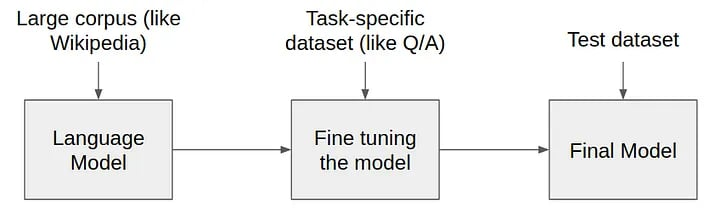
\includegraphics[width=.6\linewidth]{./assets/images/pre-train.jpeg}
    \caption{Quá trình tiền huấn luyện một mô hình.}
\end{minipage}

\subsubsection{Tổng quan}

Pretraining model đã chứng minh sự hiệu quả của nó trong nhiều ứng dụng khác nhau trong ngành IT, bao gồm xử lý ngôn ngữ tự nhiên (NLP), thị giác máy tính, dịch máy, và nhiều hơn nữa. Sự tiên tiến trong pretraining model đã đóng góp quan trọng vào việc cải thiện hiệu suất và độ chính xác của các ứng dụng AI và machine learning trong các lĩnh vực khác nhau, từ tự động hóa công việc đến y tế và kinh doanh

Với các mô hình sử dụng kiến trúc Transformer, chúng có thể sử dụng chung phần lõi của mô hình.
Sau đó, thay đổi kiến trúc hoặc cập nhật trọng số một vài tầng cuối cùng của mô hình để phục vụ cho các tác vụ khác nhau.

Đặc tính này đã cho phép các mô hình "Pretrained" ra đời. Những mô hình Pretrained Transformer này, đã được pre-train
trên một tập dữ liệu khổng lồ bởi các tập đoàn công nghệ lớn như Google, Meta, OpenAI và
được phát hành cho cộng đồng sử dụng.


\begin{minipage}{\linewidth}
    \captionsetup{type=figure}
    \centering
    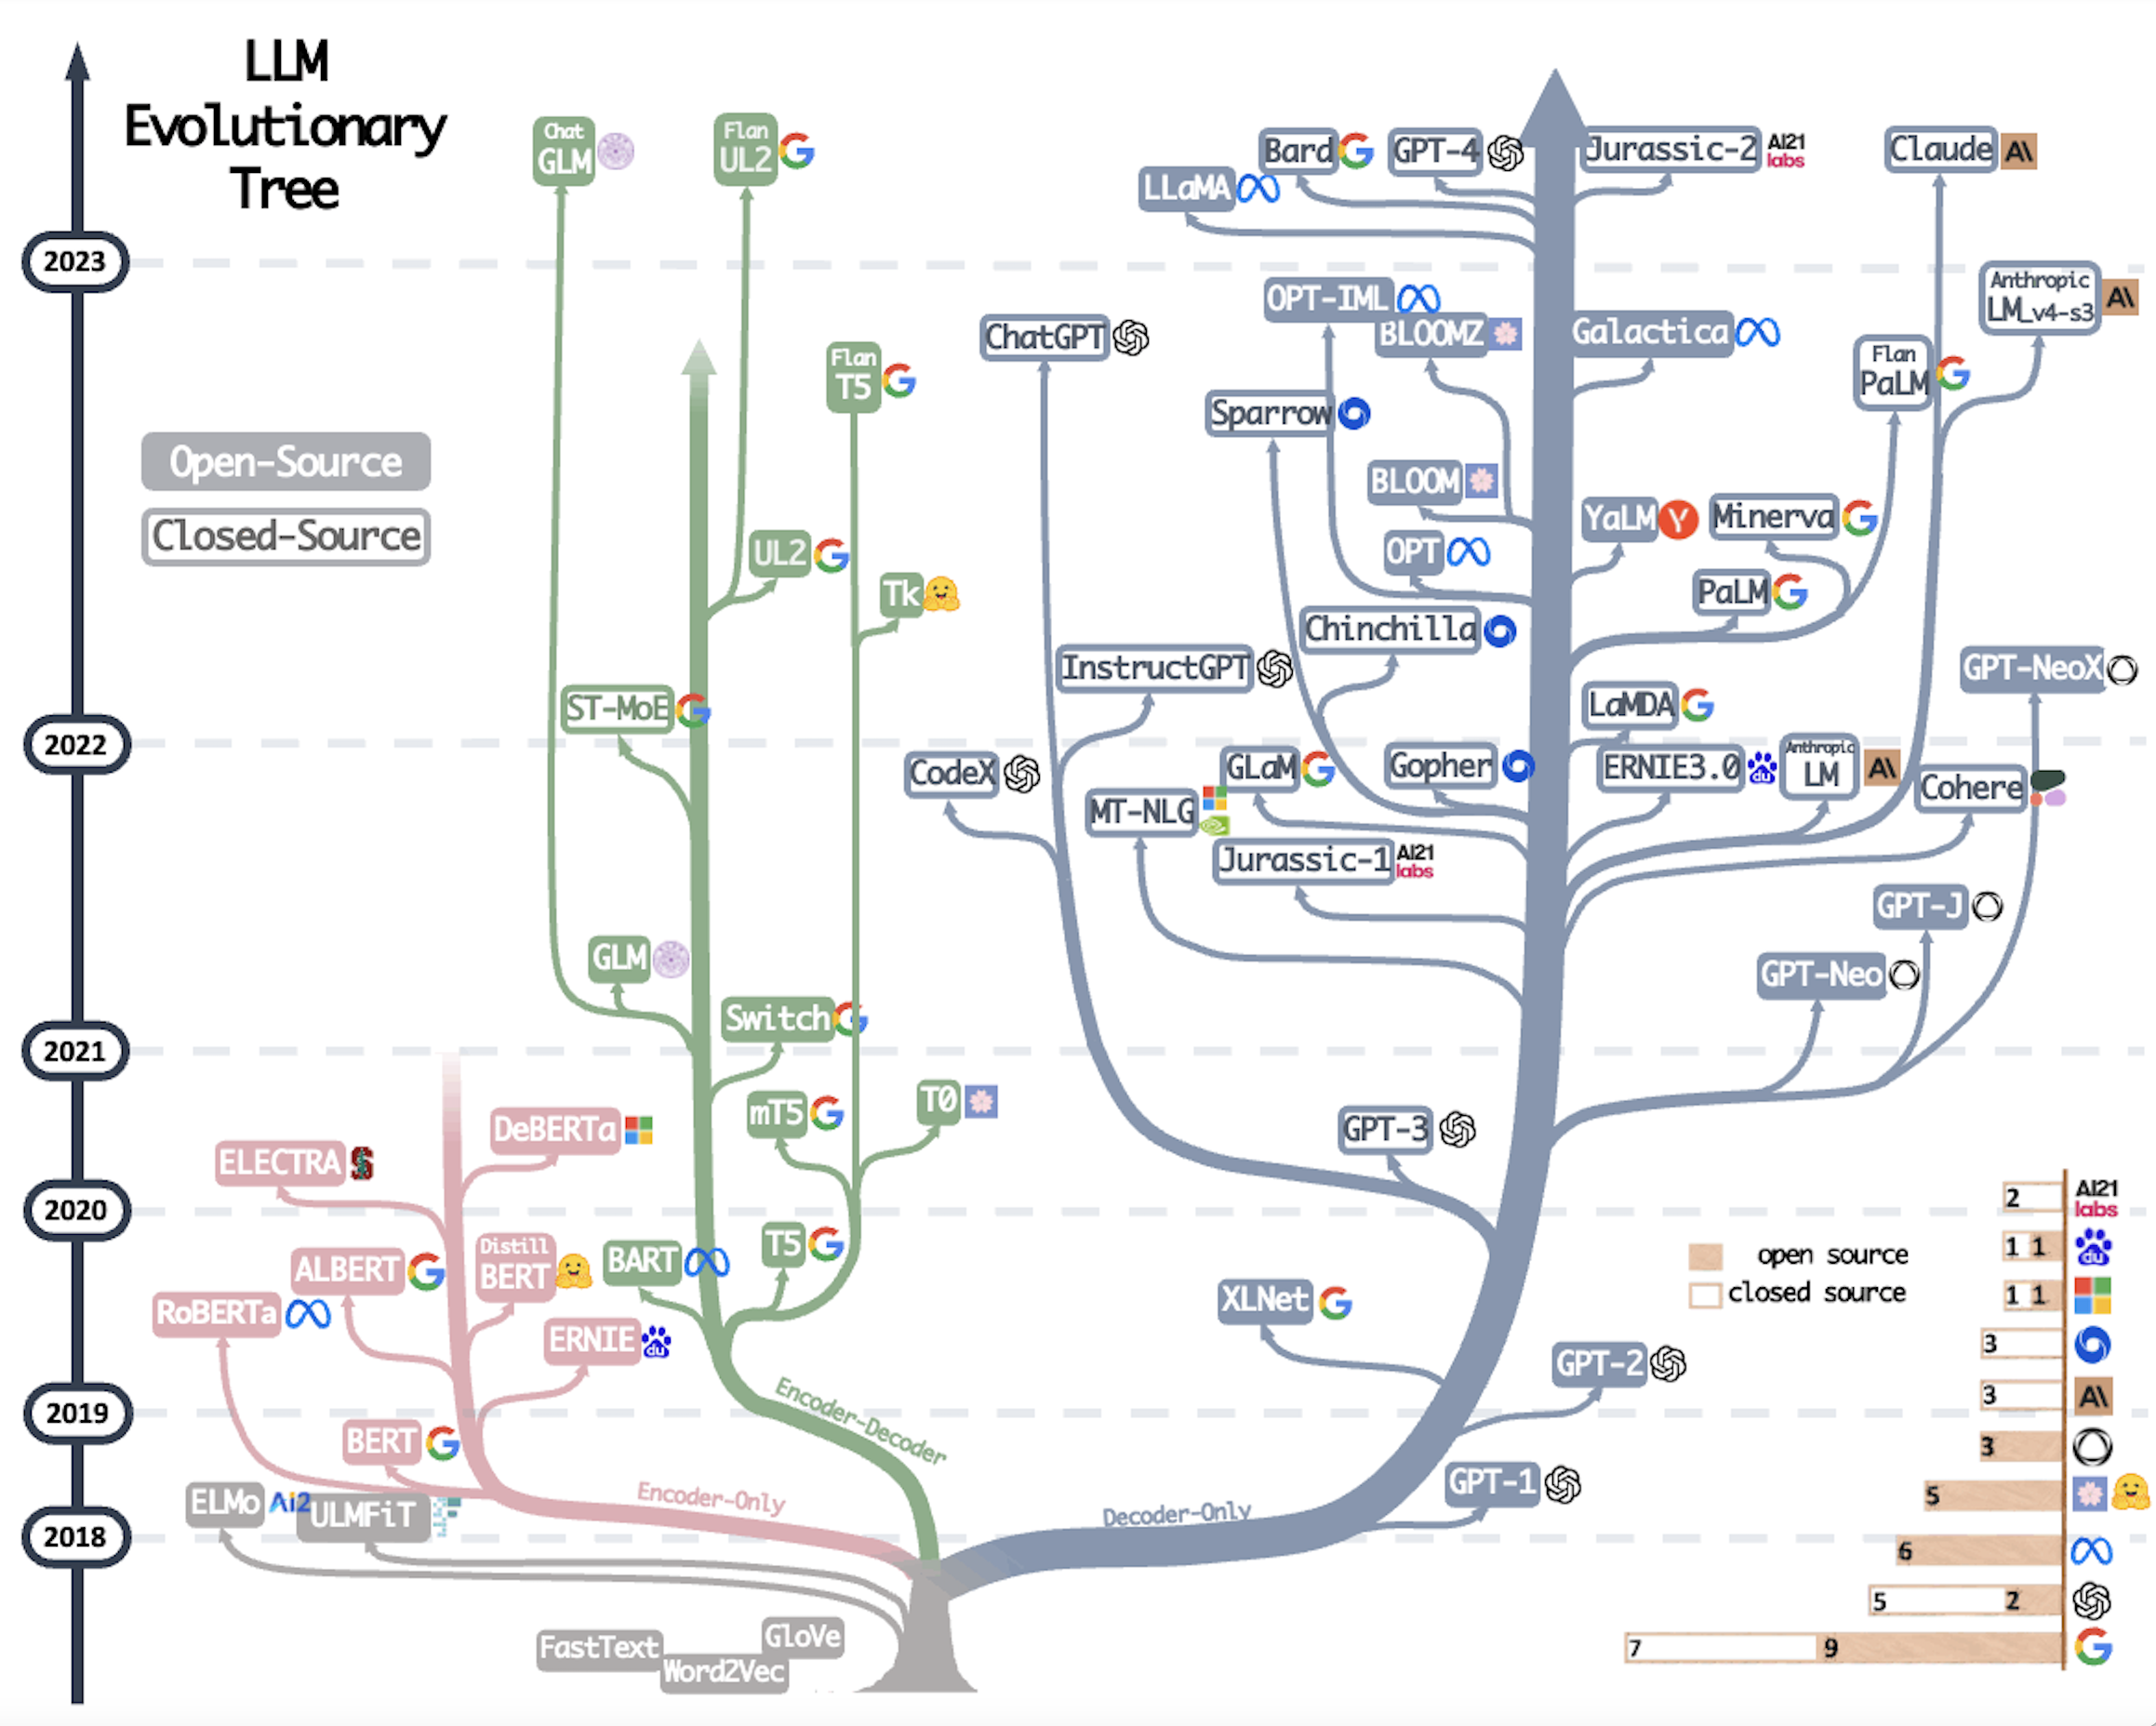
\includegraphics[width=.6\linewidth]{./assets/images/LLM-Evolutionary-Tree.png}
    \caption{Sự phát triển của các mô hình pretrained và LLm đến năm 2023\cite{llm-trends}}
\end{minipage}

\subsubsection{Các phương pháp tiền huấn luyện (pre-train) mô hình ngôn ngữ}

\textbf{Masked Language Model – MLM}

\ac{mlm} là một tác vụ được sử dụng trong quá trình
tiền huấn luyện (pre-training) của các mô hình Pretrained. Với MLM, một phần tử ngẫu nhiên trong câu
được chọn và sau đó được che đi. Mô hình sẽ nhận diện từ xung quanh từ bị che đi và cố
gắng dự đoán từ bị che đó.

Tác vụ \ac{mlm} thuộc vào bài toán tự giám sát (Self-supervised learning) - nơi mà mô hình sẽ tự đào tạo để học được
các đặc trưng bên trong của dữ liệu. Trong quá trình này, ý tưởng của nó sẽ là chuyển các bài toán học máy không được giám sát (Un-supervised learning)
thành các bài toán học có giám (Supervised learning) bằng các tự động tạo ra các nhãn cần thiết.
Điều này giúp tác vụ thuộc vào bài toán tự giám sát tận dụng được nguồn dữ liệu không có nhãn - cụ thể trong tác vụ
\ac{mlm} chính là các tập văn bản lớn trên Internet.

\begin{minipage}{\linewidth}
    \captionsetup{type=figure}
    \centering
    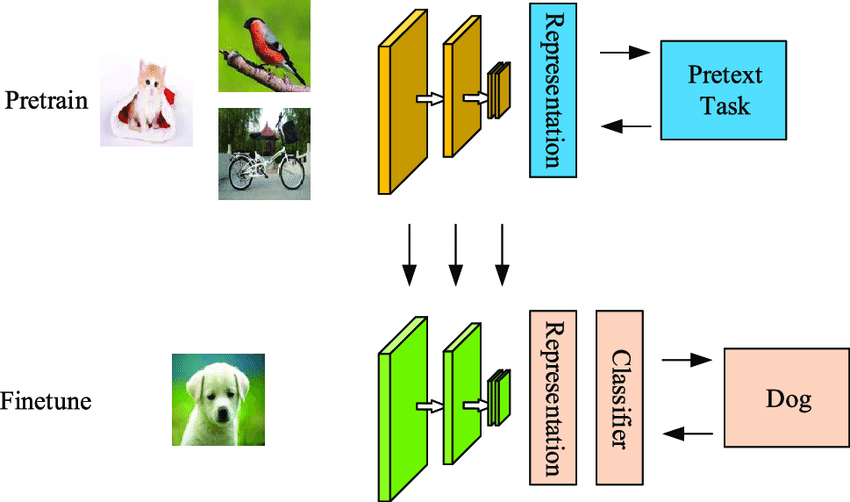
\includegraphics[width=1\linewidth]{./assets/images/self-supervised.png}
    \caption{Quá trình huấn luyện bài toán Học Tự Giám Sát\cite{balestriero2023cookbook}}
\end{minipage}

\vspace{0.5cm}

Sau khi đã kết thúc quá trình tiền huấn luyện, các mô hình trong bài toán học tự giám sát sẽ được
fine-tune lại cho một tác vụ cụ thể (downstream tasks). Từ đó cải thiện độ chính xác và năng lực của mô hình
trên các tác vụ đó.

Điều đặc biệt về cách sử dụng \ac{mlm} trong các mô hình tiền huấn luyện (Pretrained) là tất cả các từ trong câu đều có
thể được che. Trong khoảng 15\% trường hợp, từ được chọn để che sẽ được thay thế bằng token
[MASK] để đảm bảo rằng mô hình sẽ không chỉ nhớ từ đó, mà phải học cách dự đoán từ
đó bằng cách sử dụng các từ khác trong câu. Mục tiêu của mô hình là dự đoán từ được che giấu dựa trên ngữ cảnh của các từ còn lại trong câu.

\begin{minipage}{\linewidth}
    \captionsetup{type=figure}
    \centering
    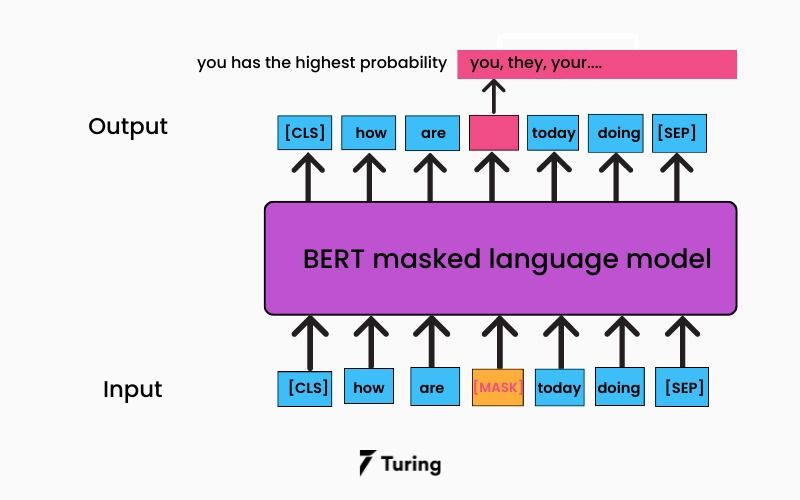
\includegraphics[width=\linewidth]{./assets/images/mllm.png}
    \caption{Masked Language Modeling\cite{mlm}}
\end{minipage}
\vspace{0.5cm}

Quá trình huấn luyện MLM không chỉ giúp mô hình học được biểu diễn của từng từ trong câu mà còn giúp nó học được mối quan hệ giữa các từ và ngữ cảnh xung quanh. Khi một từ được che giấu, mô hình phải dự đoán nó dựa trên thông tin từ các từ xung quanh, điều này thúc đẩy việc học được biểu diễn ngữ nghĩa và ngữ cảnh của từ một cách hiệu quả.

MLM đã chứng minh sự hiệu quả của mình trong nhiều ứng dụng NLP, bao gồm dịch máy, tóm tắt văn bản, phân tích cảm xúc, và nhiều hơn nữa. Kỹ thuật này đã góp phần quan trọng vào sự phát triển của các mô hình ngôn ngữ hiện đại, cung cấp cho chúng khả năng hiểu ngôn ngữ tự nhiên một cách sâu sắc và tổng quát hơn.
\begin{enumerate}
    \item \textbf{Chọn ngôn ngữ và tiền xử lý dữ liệu}: Trước hết, cần xác định ngôn ngữ của bộ dữ liệu và tiền xử lý dữ liệu, chuẩn hóa dữ liệu, và tokenize dữ liệu.
    Trong giai đoạn tiền xử lý dữ liệu cho tác vụ MLM, tập dữ liệu cần chuẩn bị chỉ bao gồm một dataset với một cột duy nhất là các đoạn văn bản:

    \begin{table}[H]
        \centering
        \begin{tabularx}{\textwidth}{|X|}
            \hline
                \textbf{Text}
            \\
            \hline
            "On its day of release in Japan , Valkyria Chronicles III topped both platform @-@ exclusive and multi @-@ platform sales charts . By early February , the game sold 102 @,@ 779 units , coming in second overall to The Last Story for the Wii . By the end of the year , the game had sold just over 152 @,@ 500 units ." \\ 
            \hline
            "In a preview of the TGS demo , Ryan Geddes of IGN was left excited as to where the game would go after completing the demo , along with enjoying the improved visuals over Valkyria Chronicles II . Kotaku 's Richard Eisenbeis was highly positive about the game , citing is story as a return to form after Valkyria Chronicles II and its gameplay being the best in the series . His main criticisms were its length and gameplay repetition , along with expressing regret that it would not be localized ." \\
            \hline
        \end{tabularx}
        \caption{Dữ liệu mẫu huấn luyện cho tác vụ MLM từ tập \textbf{wikitext} \cite{merity2016pointer}}
    \end{table}

    Trong quá trình tokenize, một phương pháp thường sử dụng cho \ac{mlm} để tiền huấn luyện mô hình ngôn ngữ là nối chuỗi (concatenation). Các từ sau khi đã tokenize
    sẽ được nối lại với nhau thành các đoạn (chunks) với độ dài cố định của mỗi đoạn là \textbf{context length} của mô hình.

    \begin{minipage}{\linewidth}
        \captionsetup{type=figure}
        \centering
        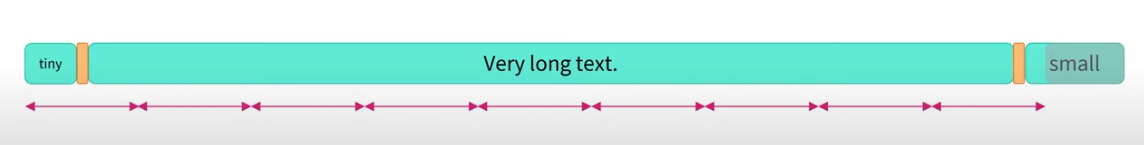
\includegraphics[width=\linewidth]{./assets/images/concatenation.png}
        \caption{Nối chuỗi dữ liệu văn bản trong quá trình pretraining}
    \end{minipage}
    \vspace{0.5cm}
    
    \item \textbf{Tạo các mẫu huấn luyện}: Tiếp theo,cần tạo ra các mẫu huấn luyện bằng cách chọn ngẫu nhiên một số từ trong mỗi câu để thực hiện Masking. Có thể cần phải chọn một phần trăm nhất định của các từ trong mỗi câu hoặc sử dụng một phương pháp khác như WordPiece hoặc Byte Pair Encoding (BPE) để chia câu thành các đơn vị từ con (subword units) và chọn ngẫu nhiên một số lượng từ con (subword) để thực hiện Masking.
    
    \item \textbf{Huấn luyện mô hình}: Sử dụng các mẫu huấn luyện đã tạo, bạn huấn luyện một mô hình MLM trên bộ dữ liệu lớn của mình. Mô hình này thường sẽ là một biến thể của mạng transformer như BERT. Trong quá trình huấn luyện, mô hình cố gắng dự đoán các từ được che giấu dựa trên ngữ cảnh của các từ xung quanh.
    
    \begin{minipage}{\linewidth}
        \captionsetup{type=figure}
        \centering
        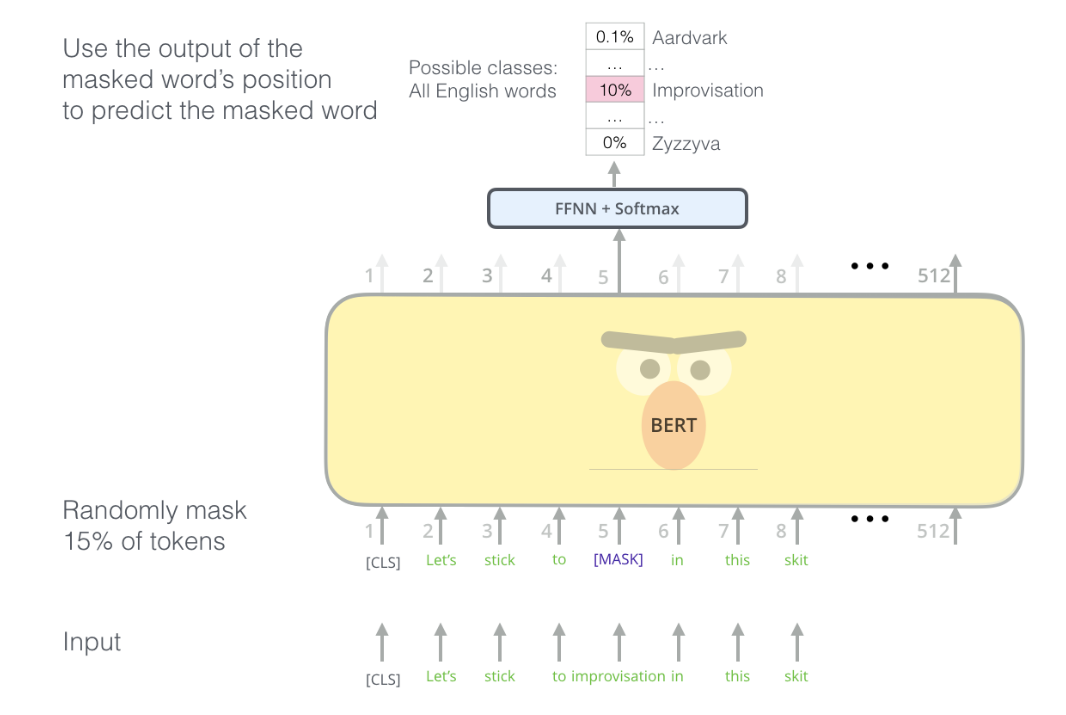
\includegraphics[width=\linewidth]{./assets/images/BERT-mlm.png}
        \caption{Tác vụ \ac{mlm} trong quá trình pretraining BERT}
    \end{minipage}
    \vspace{0.5cm}

    Với mô hình BERT, \ac{mlm} được sử dụng trong quá trình tiền huấn luyện, với 15\% số lượng token được Mask.
    Nhiệm vụ của mô hình là dự đoán các token được masked đó ở tầng kết quả (output layer).

    Hàm lỗi (loss function) lúc này sẽ chỉ tính độ lỗi dựa trên kết quả dự đoán của các Masked token chứ không phải toàn bộ tokens.

    Việc dự đoán các từ bị che ở đầu ra yêu cầu thêm các tầng để phân
    lớp (classifier) nhận đầu vào là đầu ra của BERT. Như hình, một tầng kết nối đầy đủ (Fully Connected Layer) sẽ được thêm ngay sau 
    BERT như là một tầng kết quả (output layer).
    Tiếp theo đó sẽ sử dụng softmax để tính xác suất nhằm biết được từ bị che là từ gì. Số lượng units của tầng kết quả của mạng kết nối đầy đủ 
    phải bằng với kích thước từ điển (corpus size).

\end{enumerate}

\textbf{Next Sequence Prediction – NSP hay Two-sequence tasks}

\ac{nsp} là một tác vụ quan trọng khác trong qúa trình tiền huấn luyện (pretraining) các mô hình.
Mục tiêu của \ac{nsp} là giúp mô hình hiểu được mối quan hệ giữa các câu. Nói cách
khác, các mô hình tiền huấn luyện không chỉ quan tâm đến từng câu một mà còn nhìn vào mối quan hệ giữa
các câu trong văn bản.

Trong tác vụ này, mô hình sẽ được huấn luyện trên kết quả nhị phân để quyết định xem hai câu có mối quan hệ với nhau hay không.
Điều này giúp các mô hình pretrained học được mối quan hệ cho câu trước đó.

\begin{minipage}{\linewidth}
    \captionsetup{type=figure}
    \centering
    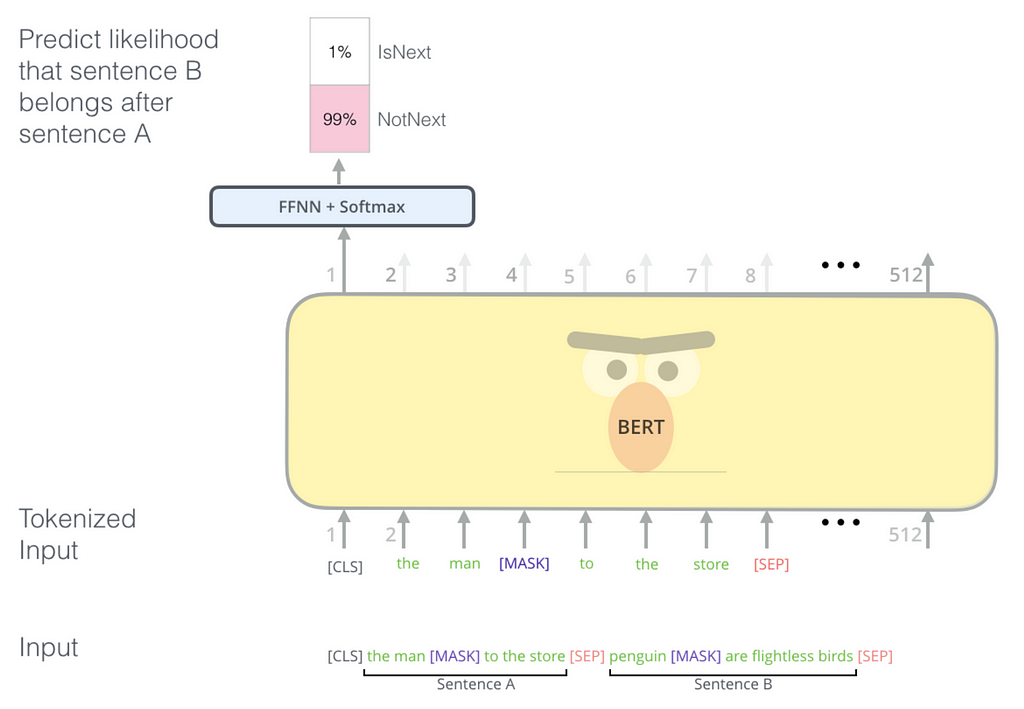
\includegraphics[width=\linewidth]{./assets/images/BERT-nsp.png}
    \caption{Tác vụ \ac{nsp} trong quá trình pretraining BERT}
\end{minipage}
\vspace{0.5cm}

Về dữ liệu cần để huấn luyện cho tác vụ \acl{nsp}, với các cặp câu A và B, để có một bộ dữ liệu cân bằng
ta cần chuẩn bị sao cho 50\% số câu B phía sau câu A sẽ có liên quan và 50\% còn lại là ngược lại.

Tương tự như tác vụ tiền huấn luyện với \acl{mlm}, kết quả đầu ra của mô hình BERT sẽ được vào một mạng kết nối đầy đủ
(Fully connected neural network) để giúp phân loại độ tương quan giữa hai câu văn bản.

\subsection{Mô hình BERT}
\subsubsection{Tổng quan mô hình}

\acl{bert} là một mô hình
ngôn ngữ tiên tiến trong lĩnh vực xử lý ngôn ngữ tự nhiên (NLP) được phát triển bởi
Google vào năm 2018. BERT được xây dựng trên kiến trúc Transformer, một mô hình học
sâu dựa trên cơ chế Attention. Mô hình này đã chứng minh sự hiệu quả của mình trong
nhiều tác vụ NLP khác nhau, bao gồm phân loại văn bản, trích xuất thông tin, dịch máy, và
trả lời câu hỏi.

\begin{minipage}{\linewidth}
    \captionsetup{type=figure}
    \centering
    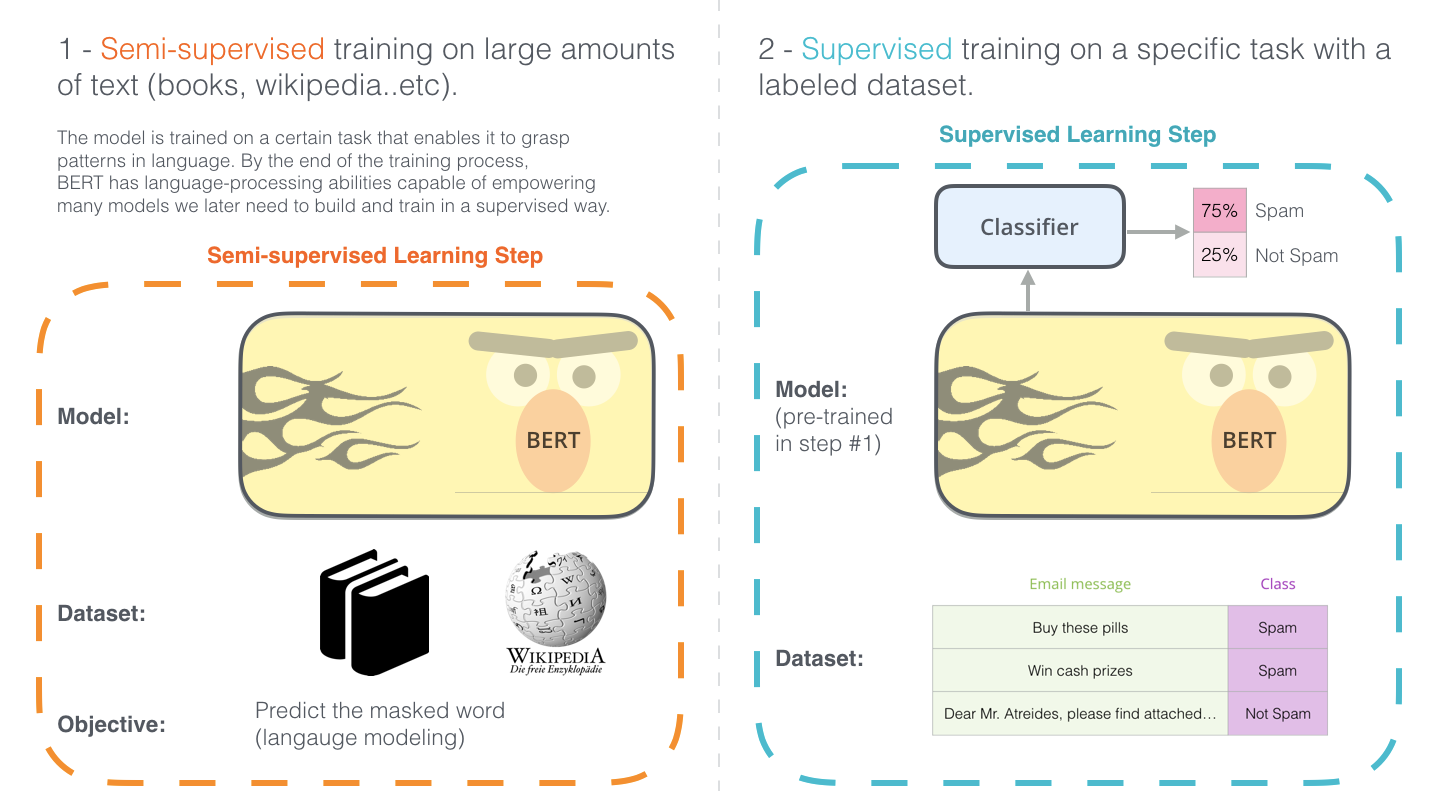
\includegraphics[width=\linewidth]{./assets/images/BERT.png}
    \caption{Mô hình BERT trong quá trình pre-training và trong quá trình fine-tuning}
\end{minipage}
\vspace{0.5cm}

BERT được huấn luyện trên một lượng lớn dữ liệu văn bản từ các nguồn khác nhau,
bao gồm các tài liệu trên web, các trang báo, tạp chí, sách và các bài báo khoa học. Quá
trình huấn luyện của BERT được thực hiện trên một tập hợp các nhiệm vụ phụ (pre-
training tasks) trước khi được fine-tuning trên các tác vụ cụ thể như phân loại văn bản,
trích xuất thông tin, hoặc dịch máy. Với việc sử dụng các pre-training tasks,
BERT có khả năng hiểu được ngôn ngữ tự nhiên một cách toàn diện hơn so với các mô
hình truyền thống.

\begin{minipage}{\linewidth}
    \captionsetup{type=figure}
    \centering
    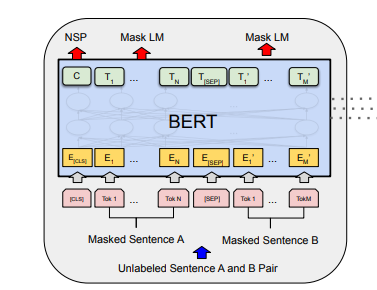
\includegraphics[width=.8\linewidth]{./assets/images/BERT-pretraining.png}
    \caption{Biểu diễn ngữ cảnh một chiều và biểu diễn ngữ cảnh hai chiều.}
\end{minipage}
\vspace{0.5cm}

BERT được huấn luyện hai tác vụ NLP khác nhau trong quá trình tiền huấn luyện  nhưng có liên quan mật thiết với nhau, đó là
Masked Language Model (MLM) và Next Sequence Prediction (NSP). Mục đích của huấn luyện MLM là ẩn đi một từ trong câu và để thuật toán dự đoán xem từ nào đã được ẩn
dựa trên ngữ cảnh. Còn mục đích của NSP nhằm dự đoán hai câu đã cho có kết nối có liên kết ngữ nghĩa
với nhau không, tuần tự không hay chỉ là ngẫu nhiên. Điều này giúp BERT đạt được kết
quả rất tốt trên nhiều tác vụ trong NLP.

\begin{minipage}{\linewidth}
    \captionsetup{type=figure}
    \centering
    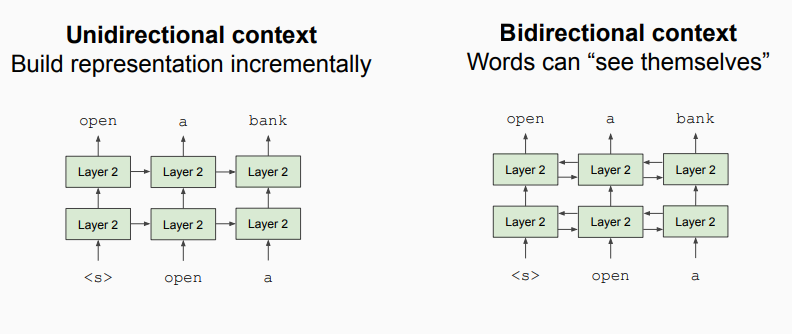
\includegraphics[width=\linewidth]{./assets/images/BERT-bidirectional.png}
    \caption{Biểu diễn ngữ cảnh một chiều và biểu diễn ngữ cảnh hai chiều.}
\end{minipage}
\vspace{0.5cm}

Một trong những điểm nổi bật của BERT là khả năng xử lý ngôn ngữ tự nhiên hai
chiều (bidirectional), có nghĩa là nó có thể hiểu được ngữ cảnh của từ cần xử lý không chỉ
dựa trên các từ trước đó mà còn dựa trên các từ sau đó. Điều này chính là một cải thiện từ
kiến trúc \textit{Unidirectional} của các mô hình trước đó như RNNs và LSTMs.

Về mặt kiến trúc, BERT là mô hình Encoder-Only Transformer, nghĩa là nó chỉ sử dụng khối Encoder của Transformer để xử lý dữ liệu.
Bài báo \textit{"BERT: Pre-training of Deep Bidirectional Transformers for Language Understanding"} \cite{devlin2019bert} đã giới thiệu hai phiên bản của BERT, đó là BERT-base và BERT-large.

\begin{minipage}{\linewidth}
    \captionsetup{type=figure}
    \centering
    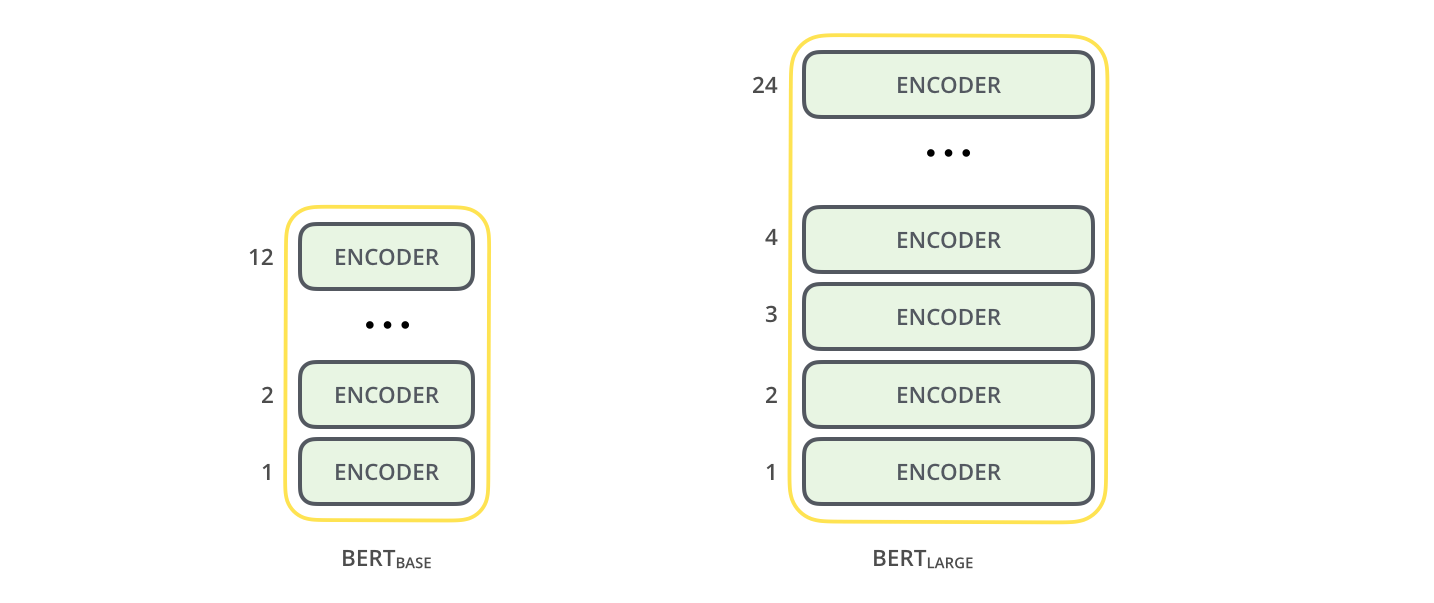
\includegraphics[width=\linewidth]{./assets/images/BERT-versions.png}
    \caption{Hai phiên bản kích thước khác nhau của mô hình BERT.}
\end{minipage}
\vspace{0.5cm}

Mô hình BERT sẽ bao gồm nhiều khối Encoder chồng lên nhau. Với BERT-base, mô hình sẽ sử dụng L = 12 khối Encoder. Trong khi đó, BERT-large sẽ sử dụng L = 24 khối Encoder.

Các thông số chính trong một mô hình BERT: L là số tầng Transformers (blocks)
được sử dụng với kích thước của các tầng ẩn là H và số lượng Scaled Dot-Product Attention
ở tầng Multi-Head Attention là A.

\begin{itemize}
    \item \(BERT_{BASE}\): L = 12, H = 768, A = 12. Tổng số tham số: 110 triệu.
    \item \(BERT_{LARGE}\): L = 24, H = 1024, A = 16. Tổng số tham số: 340 triệu.
\end{itemize}

\subsubsection{Đầu vào và đầu ra của BERT}

\begin{minipage}{\linewidth}
    \captionsetup{type=figure}
    \centering
    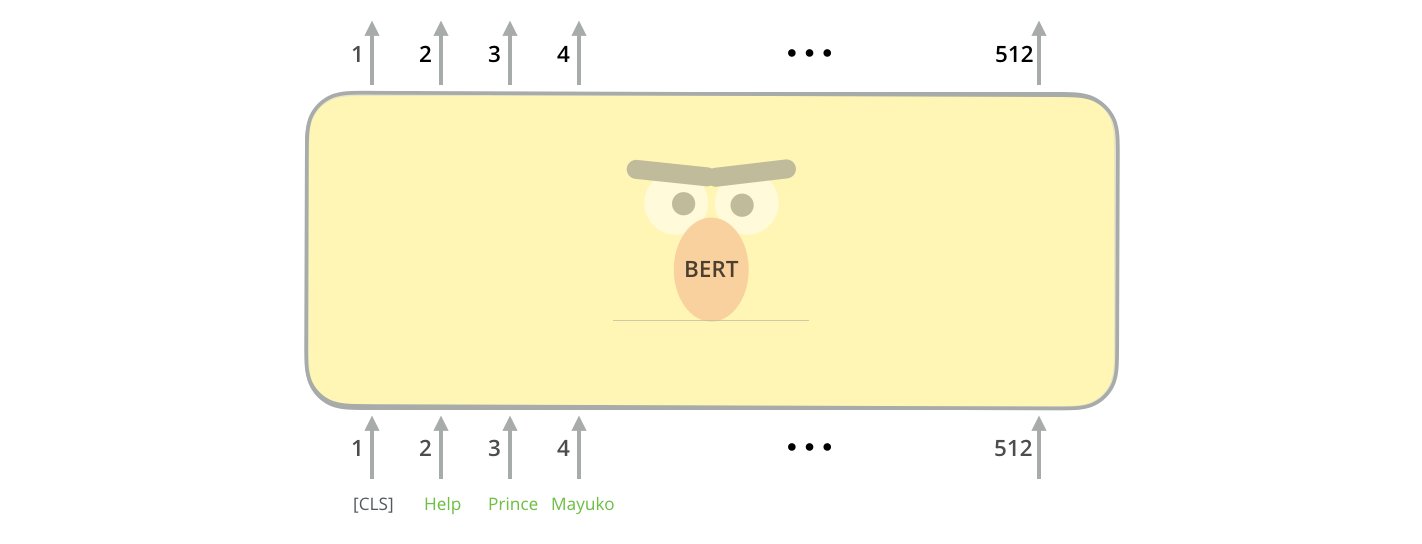
\includegraphics[width=\linewidth]{./assets/images/BERT-input.png}
    \caption{Đầu vào của mô hình BERT.}
\end{minipage}
\vspace{0.5cm}

Giống với kiến trúc Transformer, BERT sẽ nhận đầu vào là một chuỗi các token, mỗi token sẽ được biểu diễn dưới dạng một vector có kích thước cố định. 
Vector embedding này có thể được tạo ra bằng cách sử dụng các phương pháp như Word2Vec, GloVe, hoặc FastText.

Token đầu vào sẽ được thêm vào một token đặc biệt ở đầu câu [CLS] và token đặc biệt ở giữa các câu [SEP]. Và nếu
câu có độ dài ngắn hơn độ dài tối đa của mô hình, thì các vị trí còn lại sẽ được điền vào bằng token đặc biệt [PAD].

Với mỗi vị trí của token đầu vào, đầu ra của mỗi khối Encoder sẽ là một vector biểu diễn của token đó với kích thước H bằng với kích thước của embedding token đầu vào.
Với mô hình BERT-base, kích thước của vector biểu diễn token đầu ra sẽ là \(BERT_{BASE}\) = 768.

\begin{minipage}{\linewidth}
    \captionsetup{type=figure}
    \centering
    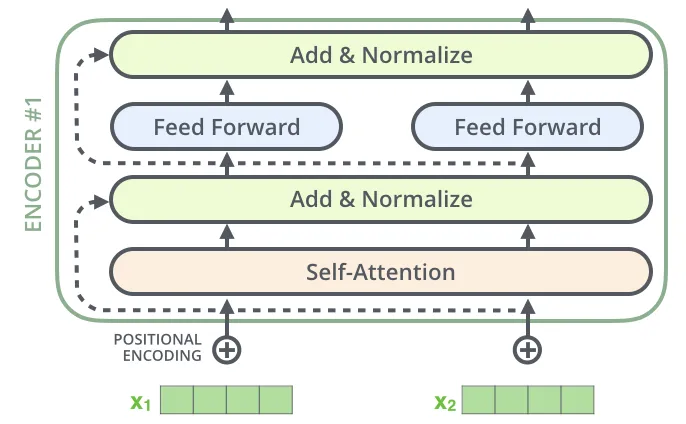
\includegraphics[width=.8\linewidth]{./assets/images/BERT-output.png}
    \caption{Đầu ra của mỗi khối encoder trong mô hình BERT.}
\end{minipage}
\vspace{0.5cm}


Với việc vector đầu vào và đầu ra có cùng kích thước, các khối Encoder có thể được xếp chồng lên nhau. Mỗi khối Encoder l + 1 sẽ nhận đầu vào từ khối Encoder l và tạo ra đầu ra cho khối Encoder l + 1.

\begin{minipage}{\linewidth}
    \captionsetup{type=figure}
    \centering
    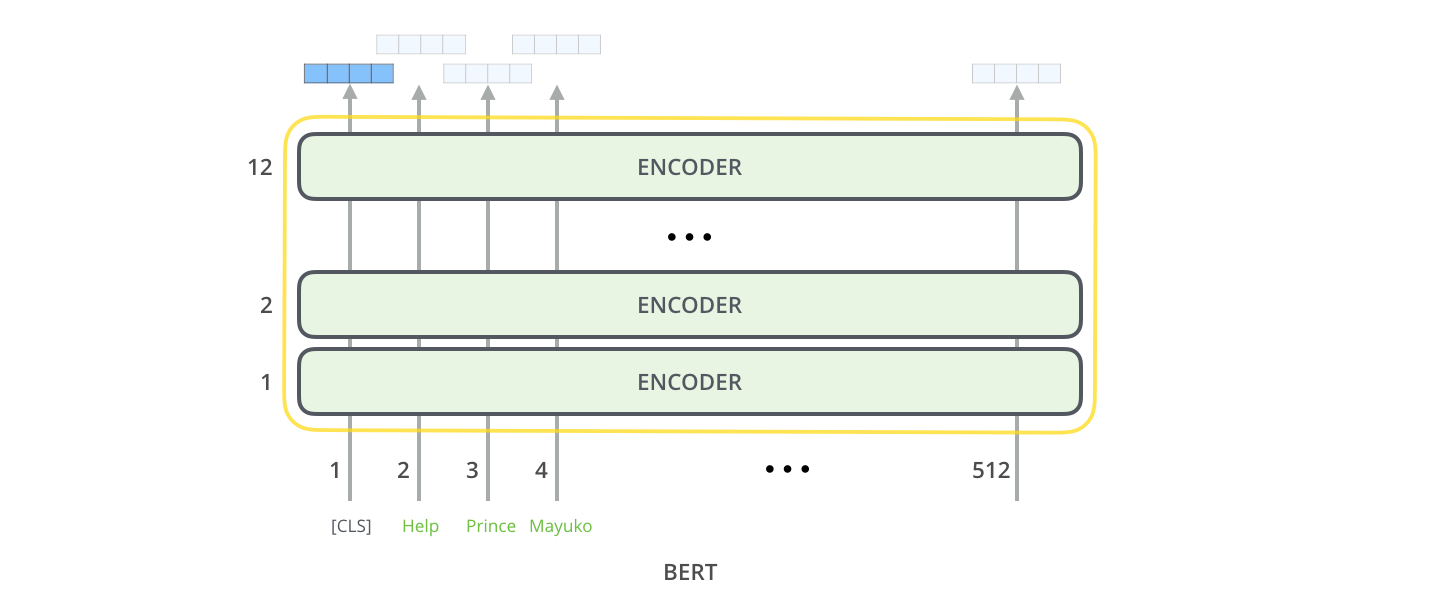
\includegraphics[width=.8\linewidth]{./assets/images/BERT-stack-encoder.png}
    \caption{Đầu ra của mỗi khối Encoder sẽ được làm đầu vào cho khối Encoder tiếp theo trong mô hình BERT.}
\end{minipage}
\vspace{0.5cm}

Đến khối cuối cùng, đầu ra của nó sẽ là biểu diễn của toàn bộ câu văn bản. Để thực hiện các tác vụ cụ thể như phân loại văn bản, trích xuất thông tin, hoặc dịch máy, một tầng kết nối đầy đủ (Fully Connected Layer) sẽ được thêm vào cuối cùng để phân loại hoặc dự đoán kết quả. 

Với bài toán phân loại văn bản, ta chỉ cần sử dụng vector biểu diễn của token đặc biệt [CLS] ở đầu câu để thực hiện phân loại như sau:

\begin{minipage}{\linewidth}
    \captionsetup{type=figure}\    
    \centering
    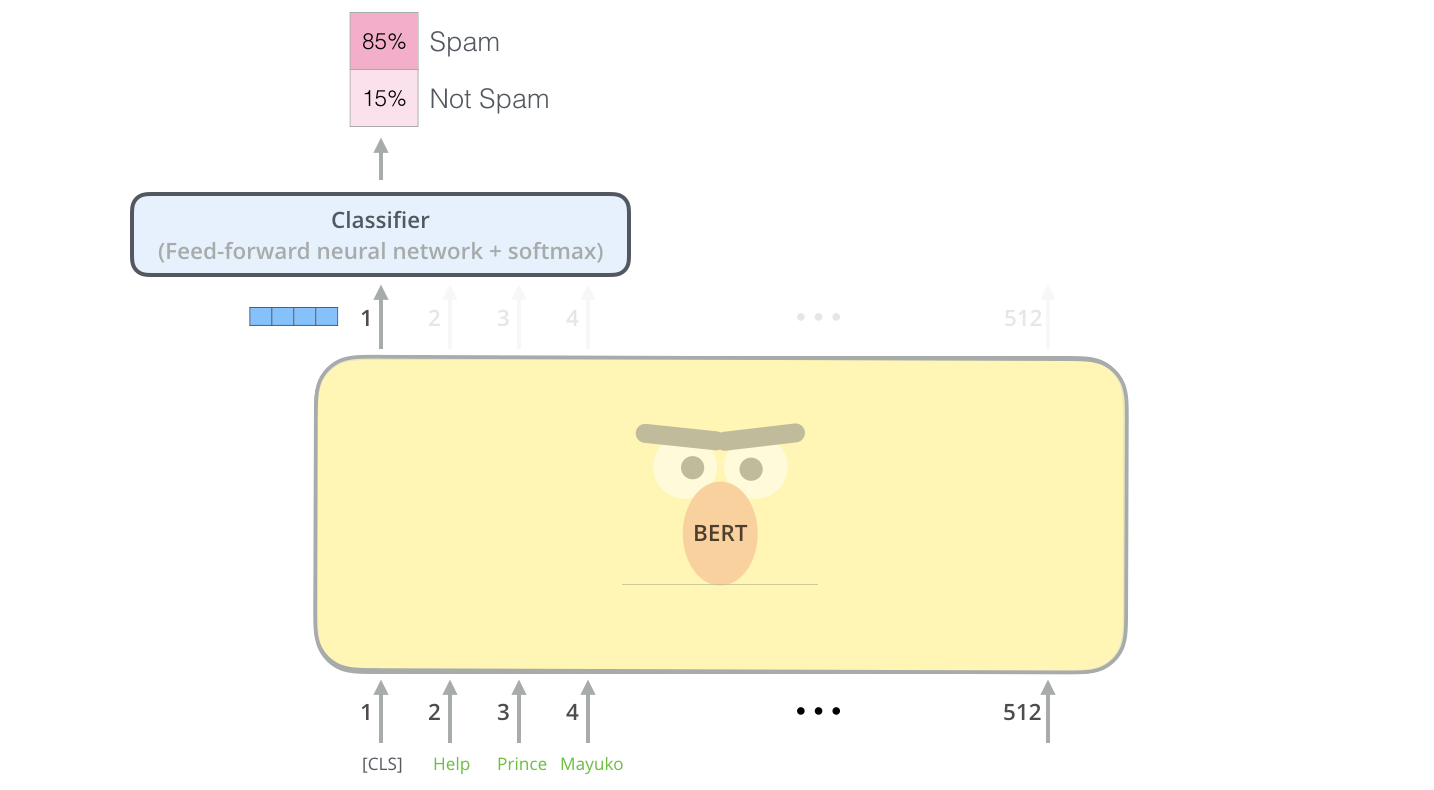
\includegraphics[width=.8\linewidth]{./assets/images/BERT-classification.png}
    \caption{Đầu ra của mỗi khối Encoder sẽ được làm đầu vào cho khối Encoder tiếp theo trong mô hình BERT.}
    \label{fig:bert_classification}
\end{minipage}
\vspace{0.5cm}

Hình \ref{fig:bert_classification} trình bày việc sử dụng vector đại diện cho [CLS] token ở đầu ra để phân lớp
một bài toán có hai nhãn “Spam”, “Not Spam” sử dụng SLP với hàm kích hoạt là Softmax.
Nếu chúng ta có nhiều hơn hai nhãn, ví dụ, đối với bài toán có các nhãn “Spam”, “Not Spam”, “Social” và “Promotion”, thì chỉ cần tuỳ
chỉnh số lượng neuron ở đầu ra của SLP

\subsubsection{Trích xuất đặc trưng từ mô hình BERT}

Phương pháp fine-tuning không phải là cách duy nhất để sử dụng BERT, chúng ta
có thể sử dụng BERT đã được pre-trained để tạo ra các contextualized word embedding.

Trong quá trình huấn luyện BERT, mỗi từ trong câu đầu vào được mã hóa dưới dạng
một vector đặc trưng bằng cách sử dụng đầu ra của các tầng Encoder. Điều này cho phép
mỗi từ được biểu diễn như là một vector đặc trưng phụ thuộc vào ngữ cảnh của từ đó
trong câu. Các vector đặc trưng này được gọi là các contextualized word embeddings, và
chúng có thể được sử dụng để biểu diễn các từ trong các tác vụ xử lý ngôn ngữ tự nhiên
khác nhau.

\begin{minipage}{\linewidth}
    \captionsetup{type=figure}
    \centering
    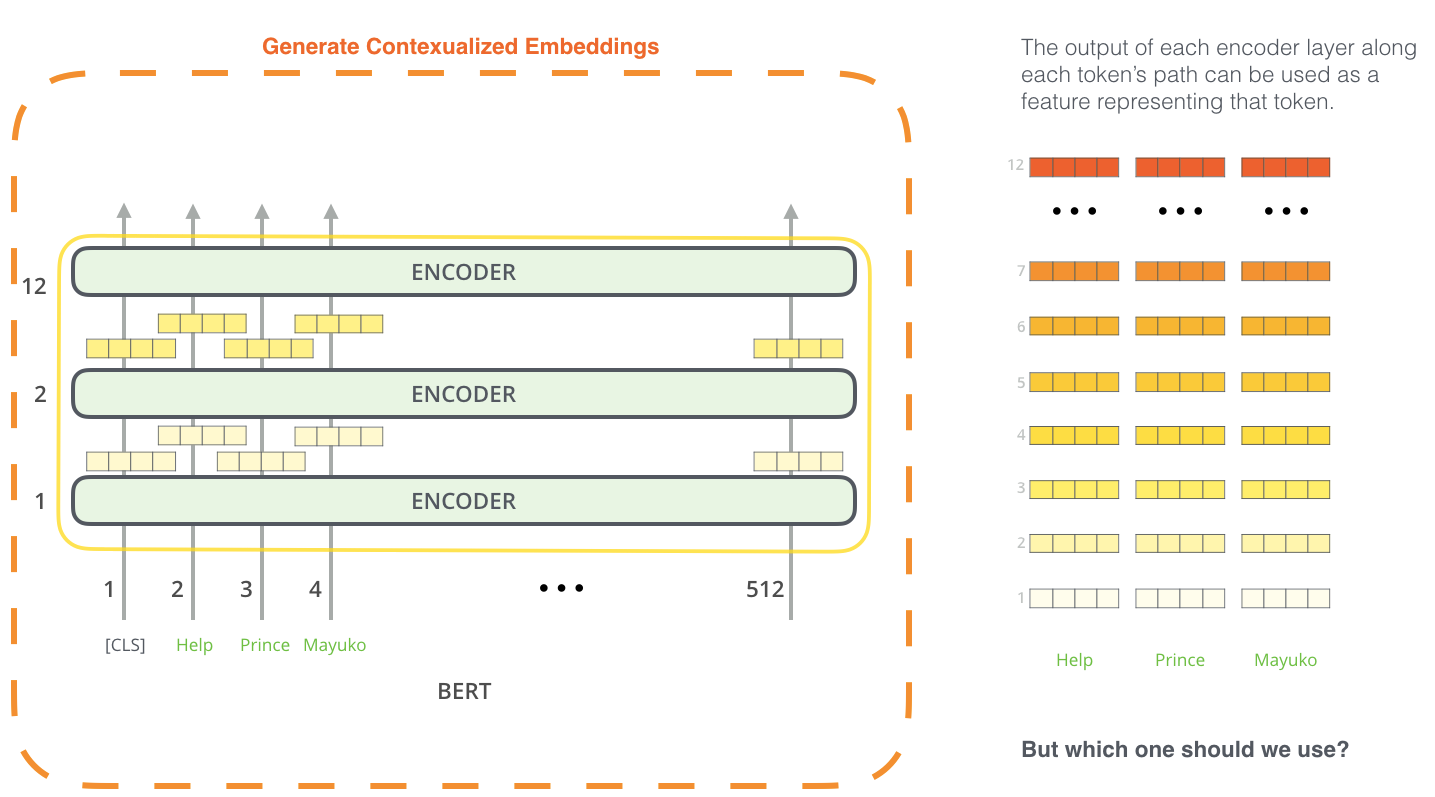
\includegraphics[width=.8\linewidth]{./assets/images/BERT-context1.png}
    \caption{Trích xuất đặc trưng sử dụng BERT.}
    \label{fig:bert_context1}
\end{minipage}
\vspace{0.5cm}

Đầu ra của mỗi tầng Encoder trên đường đi của mỗi từ có thể được sử dụng như
một đặc trưng đại diện cho từ đó \ref{fig_bert_context1}. Vậy đâu là sự lựa chọn tốt nhất để dùng làm
contextualized embedding. Ta có thể xem xét sáu lựa chọn bên dưới, với thông số đánh giá là 
Dev F1-score.

\begin{minipage}{\linewidth}
    \captionsetup{type=figure}
    \centering
    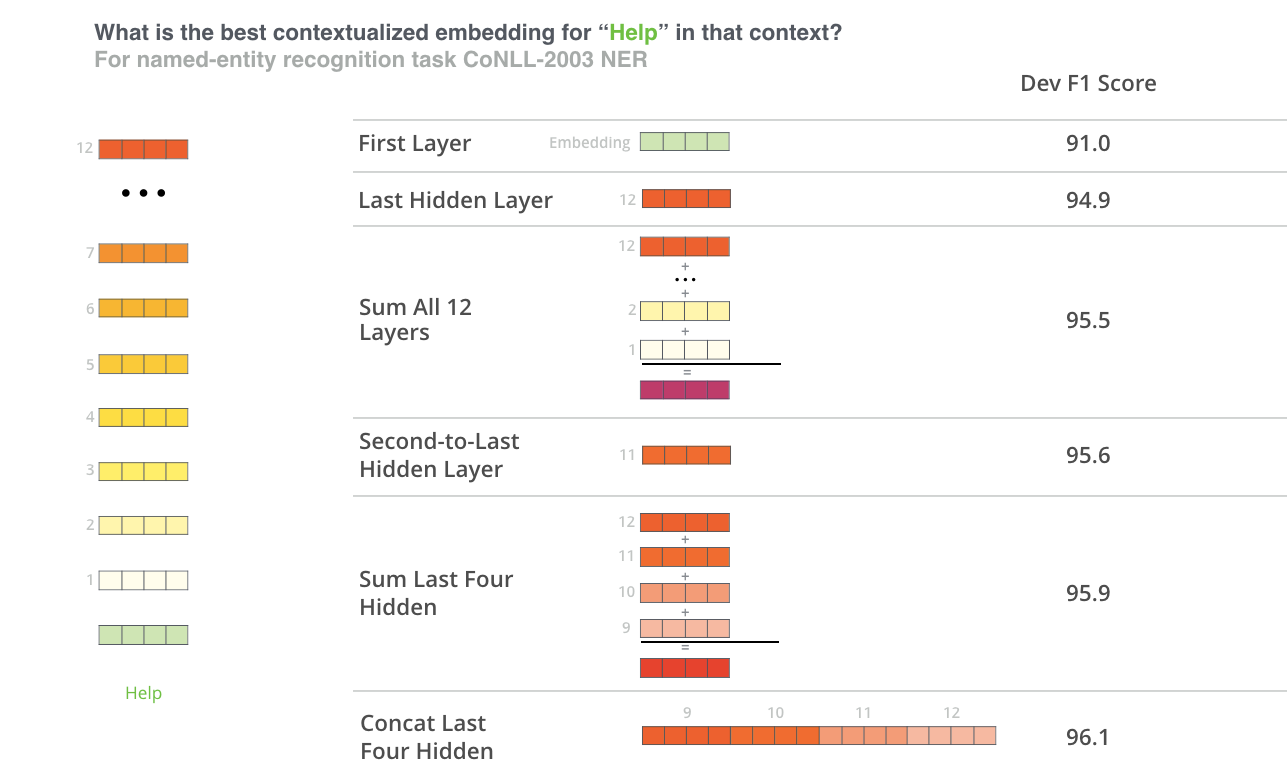
\includegraphics[width=.8\linewidth]{./assets/images/BERT-context2.png}
    \caption{Lựa chọn vector embedding từ đặc trưng sử dụng BERT.}
    \label{fig:bert_context2}
\end{minipage}
\vspace{0.5cm}

Dev F1-score là một chỉ số đánh giá hiệu suất của mô hình trong quá trình đánh giá (validation) trên tập dữ liệu kiểm
tra. Nó được tính bằng cách sử dụng công thức F1-score trên tập dữ liệu kiểm tra và được sử dụng để so sánh và đánh
giá hiệu suất của các mô hình khác nhau trong cùng một tác vụ. Chỉ số này càng cao thì mô hình càng tốt.

\subsubsection{Sử dụng BERT để so sánh sự tương đồng ngữ nghĩa}

Với đầu ra của mô hình BERT là một ma trận biểu diễn của toàn bộ câu văn bản, chúng ta có thể sử dụng ma trận này để so sánh sự tương đồng ngữ nghĩa giữa các câu.
Ta có thể dựa vào kiến trúc của mô hình Cross-encoder để so sánh sự tương đồng ngữ nghĩa giữa các câu như sau:

\begin{minipage}{\linewidth}
    \captionsetup{type=figure}
    \centering
    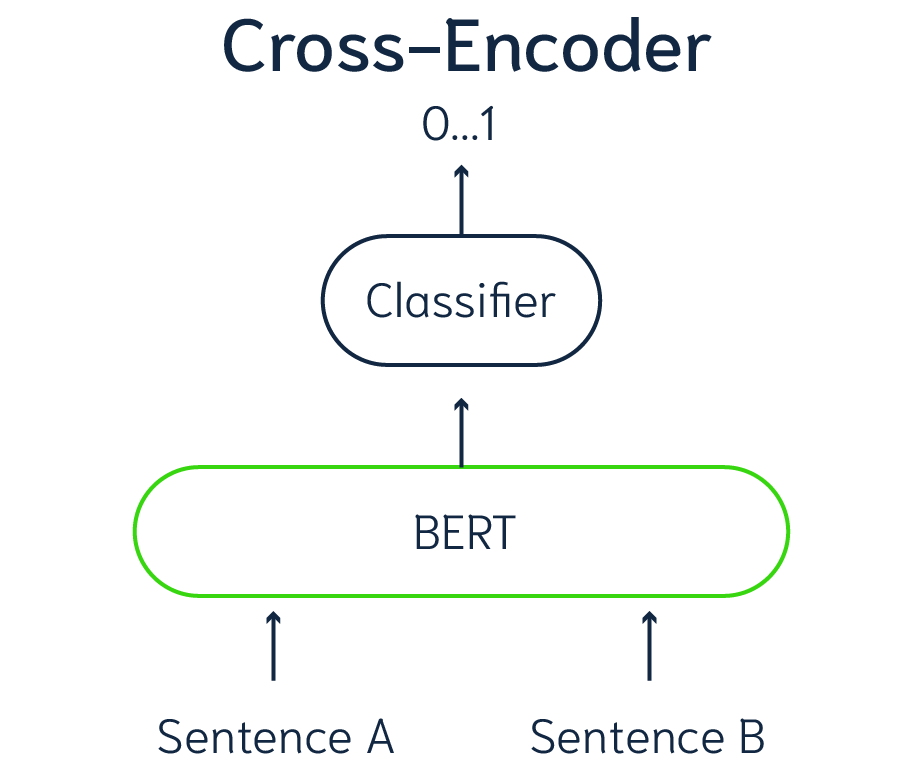
\includegraphics[width=.8\linewidth]{./assets/images/cross-encoder.png}
    \caption{So sánh sự tương đồng ngữ nghĩa giữa các câu với mô hình BERT.}
\end{minipage}
\vspace{0.5cm}

Trong một tập với n câu văn bản, ta có thể xét từng cặp câu và cho chúng vào cùng lúc với mô hình Cross-encoder sử dụng BERT.
Hai câu văn bản sẽ được nối lại với nhau, và phân cách bằng một token đặc biệt [SEP]. Sau đó, chúng sẽ được đưa vào mô hình BERT để tạo ra biểu diễn của cả hai câu.

Ma trận biểu diễn này của cả hai câu sau đó sẽ được đưa vào một tầng kết nối đầy đủ (Fully Connected Layer) để dự đoán độ tương đồng ngữ nghĩa giữa nó.
Tầng Classifier này sẽ trả về nhãn là một giá trị số thực trong khoảng [0, 1] thể hiện độ tương đồng ngữ nghĩa giữa hai câu.

Đầu vào của tầng Classifier này chỉ cần lấy vector biểu diễn của token đặc biệt [CLS] ở đầu ra của mô hình BERT để thực hiện dự đoán.

Việc xét từng cặp câu với mô hình Cross-encoder này
mang lại độ chính xác cao trong việc so sánh sự tương đồng ngữ nghĩa giữa các câu. Tuy nhiên, trong một hệ thống với rất nhiều câu văn bản, việc xét từng cặp câu sẽ dẫn đến tiêu tốn rất nhiều thời gian và
tài nguyên tính toán. Vì vậy, mô hình Cross-encoder chỉ nên đóng vai trò xếp hạng trên một tập nhỏ các câu văn bản. Ta có một ví dụ như sau:

\begin{minipage}{\linewidth}
    \captionsetup{type=figure}
    \centering
    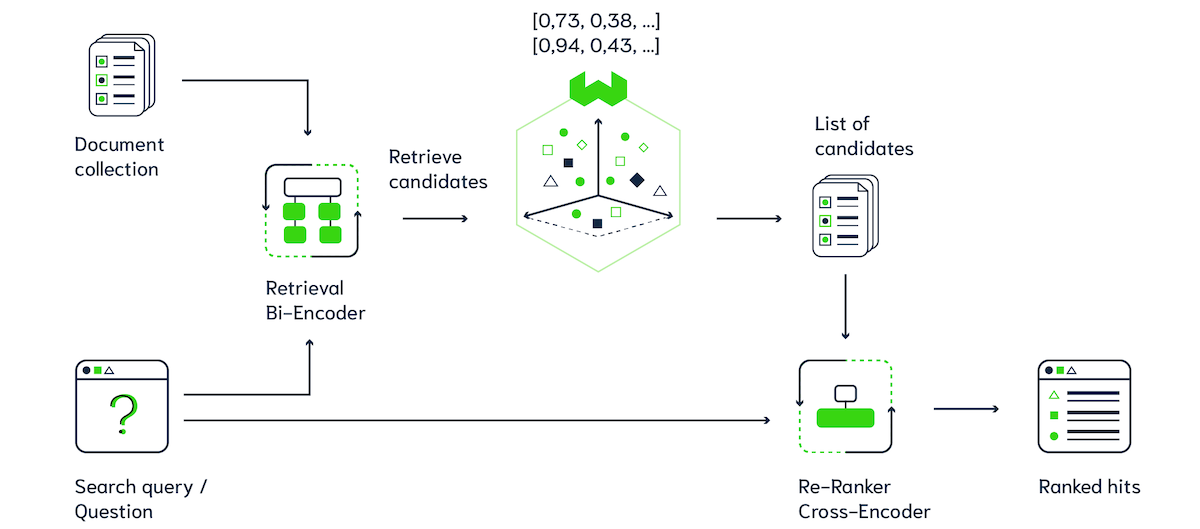
\includegraphics[width=.8\linewidth]{./assets/images/weaviate-pipeline-long.png}
    \caption{So sánh sự tương đồng ngữ nghĩa giữa các câu với mô hình BERT.}
\end{minipage}
\vspace{0.5cm}


\subsection{Độ tương đồng ngữ nghĩa Cosine giữa các embedding}

Trong lĩnh vực xử lý ngôn ngữ tự nhiên, một embedding là một biểu diễn vector của một chuỗi, được tạo ra bởi một mô hình học máy. Embedding có thể được tạo ra bằng cách sử dụng các mô hình học máy như Word2Vec, GloVe, FastText, và nhiều mô hình khác.
Ngoài ra, với sự phát triển của các mô hình học sâu và kiến trúc transformer, các embedding có thể được tạo ra bằng cách sử dụng khối encoder các mô hình sử dụng kiến trúc transformer hoặc các mô hình học sâu BERT, GPT, và nhiều mô hình khác.

Để đánh giá độ tương đồng giữa các embedding, chúng ta cần một phương pháp đánh giá độ tương đồng. Một trong những phương pháp đánh giá độ tương đồng giữa các embedding đó là độ tương đồng cosin. Công thức tính độ tương đồng cosin giữa hai embedding $A$ và $B$ được tính như sau:

\begin{equation}
    \text{similarity}(A, B) = \cos(\theta) = \frac{A \cdot B}{\|A\| \|B\|}
\end{equation}

\begin{minipage}{\linewidth}
    \captionsetup{type=figure}
    \centering
    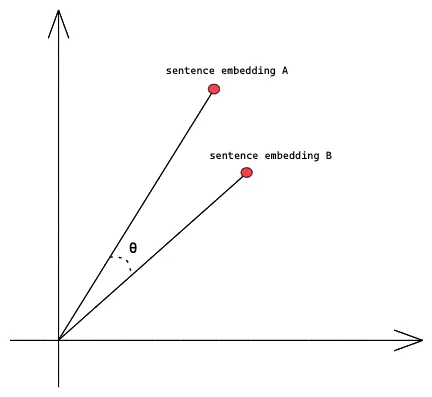
\includegraphics[width=.6\linewidth]{./assets/images/cosine.png}
    \caption{Biểu diễn công thức khoảng cách cosine giữa hai vector trên hệ tọa độ 2D.}
\end{minipage}
\vspace{0.5cm}

Một số ưu điểm khi sử dụng độ tương đồng cosin để đánh giá độ tương đồng giữa các embedding:
\begin{enumerate}
    \item \textbf{Không Ảnh Hưởng bởi Độ Dài:} Một trong những ưu điểm chính của độ tương đồng cosine là nó không bị ảnh hưởng bởi độ dài của vectơ. Bất kể kích thước của các vectơ, chỉ cần hướng của chúng giống nhau, độ tương đồng cosine sẽ là nhỏ nhất khi chúng đối lập và lớn nhất khi chúng trùng hướng.

    \item \textbf{Đo Lường Hướng Tương Đồng:} Độ tương đồng cosine tập trung vào hướng của vectơ thay vì giá trị tuyệt đối. Điều này làm cho nó thích hợp cho các tác vụ như phân loại văn bản, xác định chủ đề, và tìm kiếm tương đồng ngữ cảnh.

    \item \textbf{Hiệu Quả Cho Dữ Liệu Nhiều Chiều:} Trong không gian chiều cao, nơi mỗi chiều biểu diễn một đặc trưng khác nhau, độ tương đồng cosine thường hiệu quả hơn so với các phương pháp đo tương đồng khác. Điều này giúp giảm hiệu ứng "hiệu ứng chiều cao" khi sử dụng các phương pháp dựa trên khoảng cách Euclidean.
\end{enumerate}

\subsection{Siamese Networks}

\begin{minipage}{\linewidth}
    \captionsetup{type=figure}
    \centering
    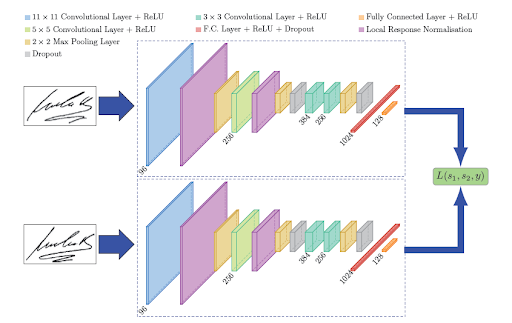
\includegraphics[width=10cm]{./assets/images/1_siamese-network.png}
    \caption{Siamese Networks\cite{https://builtin.com/machine-learning/siamese-network}}
\end{minipage} 

Mạng Siamese là một kiến trúc mạng nơ-ron đặc biệt được thiết kế để xác định mức độ tương đồng giữa hai đối tượng hoặc hai đầu vào. Đặc điểm chính của mạng Siamese là sử dụng hai nhánh đồng nhất (tương tự nhau) chia sẻ trọng số, mỗi nhánh xử lý một đầu vào khác nhau. Mục tiêu của mạng Siamese là học cách biểu diễn và so sánh đặc trưng giữa các cặp đối tượng.

Mạng Siamese thường được sử dụng trong các nhiệm vụ như nhận dạng khuôn mặt, phân loại văn bản, hay tìm kiếm hình ảnh, văn bản tương đồng. Để đạt được mục tiêu này, mạng Siamese thực hiện các bước cơ bản như sau:

\begin{itemize}
    \item[--] \textbf{Trích Xuất Đặc Trưng:} Mỗi nhánh của mạng Siamese nhận một đầu vào và trích xuất đặc trưng từ đối tượng đó bằng cách sử dụng các lớp tích chập và lớp pooling.

    \item[--] \textbf{So Sánh Đặc Trưng:} Các đặc trưng được trích xuất từ cả hai nhánh sau đó được so sánh để đo lường mức độ tương đồng giữa chúng. Thông thường, một hàm khoảng cách như Euclidean hoặc độ tương đồng cosine được sử dụng để đo lường khoảng cách giữa hai vectơ đặc trưng.

    \item[--] \textbf{Huấn Luyện và Tối Ưu Hóa:} Mạng Siamese được huấn luyện bằng cách sử dụng các cặp dữ liệu huấn luyện được gán nhãn với thông tin về mức độ tương đồng. Mục tiêu là tối ưu hóa mô hình để đặc trưng của các cặp giống nhau gần nhau và của các cặp khác nhau xa nhau.
\end{itemize}

Mạng SNN tập trung vào việc cải thiện embedding sao cho các lớp giống nhau sẽ nằm gần nhau hơn. Với việc phải bình phương số lượng dữ liệu để tạo ra các cặp so sánh, việc huấn luyện nó sẽ mất thời gian hơn là phân lớp thông thường.
Chi tiết cách huấn luyện mạng SNN như sau:

\begin{enumerate}
    \item \textbf{Xây dựng kiến trúc mạng}  Đầu tiên, chúng ta cần xác định kiến trúc của mạng nơ-ron SNN bao gồm các lớp nơ-ron và kết nối giữa chúng. Sau đó, chọn hàm loss phù hợp để đo lường sự chênh lệch giữa dự đoán và giá trị thực tế, cùng với một optimizer để cập nhật các trọng số của mạng.
    \item \textbf{Đưa dữ liệu vào cặp mạng} Tiếp theo, chúng ta cần đưa dữ liệu vào mạng SNN. Dữ liệu này thường được chia thành các cặp, mỗi cặp gồm hai phần tử tương ứng với dữ liệu đầu vào và đầu ra mong muốn.
    \item \textbf{Tính toán lỗi}  Dựa trên đầu ra của mạng cho cả hai dữ liệu đầu vào, chúng ta tính toán lỗi bằng cách so sánh dự đoán với giá trị thực tế. Lỗi này thường được tính bằng hàm loss đã chọn ở bước đầu tiên.
    
        Một số hàm lỗi phổ biến được sử dụng để đo lường sự chênh lệch giữa hai câu (hoặc văn bản) trong kiến trúc mạng Siamese có thể kể đến như sau:    
        \begin{itemize}
            \item \textbf{Hinge Loss:}  Hàm mất mát này thường được sử dụng trong các bài toán học có giám sát, đo lường khoảng cách giữa các vector nhúng của các cặp câu. Mục tiêu là tối thiểu hóa khoảng cách giữa các câu cùng loại và tối đa hóa khoảng cách giữa các cặp câu không cùng loại.
            \item \textbf{Constrative loss} Hàm mất mát này đo lường sự tương đồng giữa các cặp câu bằng cách đo khoảng cách giữa các vector nhúng và áp dụng ngưỡng để xác định xem các câu là giống nhau hay khác biệt.
            Các cặp câu chỉ có thể có hai nhãn là \textbf{0 và 1} để quyết định hai câu hoặc văn bản có tương đồng hay không.

            \begin{minipage}{\linewidth}
                \captionsetup{type=figure}
                \centering
                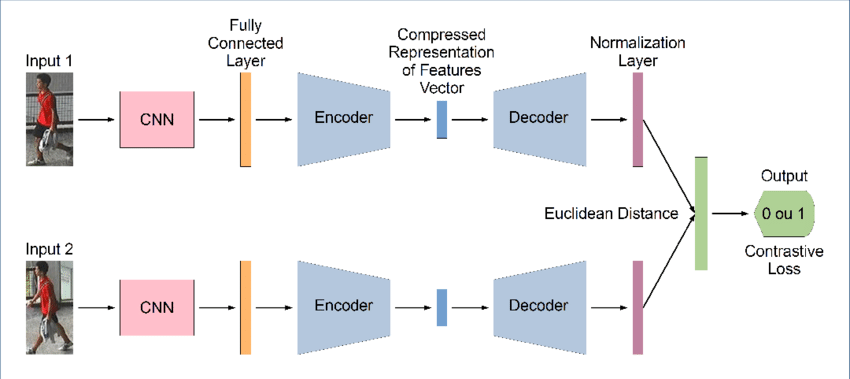
\includegraphics[width=12cm]{./assets/images/siamese-cnn.png}
                \captionof{figure}{Một ví dụ áp dụng mạng Siamese với mô hình \ac{cnn} và Constrative Loss}
            \end{minipage}

            \item \textbf{Triplet loss} Triplet loss sử dụng ba câu trong mỗi lần huấn luyện: câu anchor, câu dương (positive), và câu âm (negative). Mục tiêu là tối thiểu hóa khoảng cách giữa câu anchor và câu dương, đồng thời tối đa hóa khoảng cách giữa câu anchor và câu âm một lượng nhất định. Triplet loss thường được sử dụng khi có sẵn dữ liệu nhãn câu tương đồng và không tương đồng.
            
            \begin{minipage}{\linewidth}
                \captionsetup{type=figure}
                \centering
                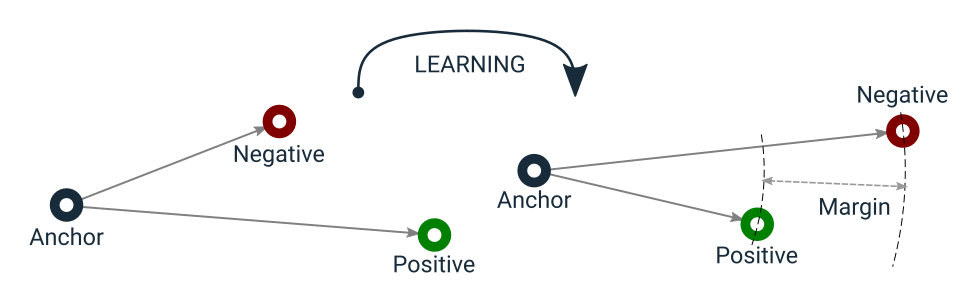
\includegraphics[width=12cm]{./assets/images/triplet.png}
                \captionof{figure}{Minh họa hàm mất mát Constrative Loss}
            \end{minipage}

            \item \textbf{Cosine similarity loss} Hàm mất mát này đo lường sự tương đồng giữa các cặp câu bằng cách sử dụng cosine similarity giữa các vector nhúng của chúng. Mục tiêu là tối đa hóa cosine similarity giữa các cặp câu giống nhau và tối thiểu hóa cosine similarity giữa các cặp câu không giống nhau. Khác biệt chính giữa cosine similarity loss và các hàm lỗi khác là cách đo đạc sự tương đồng dựa trên góc giữa hai vector nhúng, thay vì khoảng cách Euclidean.
        \end{itemize}
    \item \textbf{Lan truyền ngược} Sau khi tính được lỗi, chúng ta sử dụng phương pháp lan truyền ngược để tính toán đạo hàm của lỗi theo các trọng số của mạng. Điều này giúp chúng ta biết được hướng và mức độ điều chỉnh các trọng số để giảm thiểu lỗi.
    \item \textbf{Cập nhật trọng số} Cuối cùng, sử dụng optimizer đã chọn để cập nhật các trọng số của mạng dựa trên đạo hàm tính được từ lan truyền ngược. Quá trình này được lặp lại cho đến khi đạt được điều kiện dừng hoặc số lượng vòng lặp quy định.
\end{enumerate}

\subsection{Mô hình SBERT}

\subsubsection{Tổng quan kiến trúc các mô hình SBERT}
SBERT , hay Sentence-BERT, là một tiến bộ quan trọng trong lĩnh vực xử lý ngôn ngữ tự nhiên (NLP) và biểu diễn văn bản. Được phát triển dựa trên ý tưởng của BERT (Bidirectional Encoder Representations from Transformers), SBERT tập trung vào việc tối ưu hóa biểu diễn cho các câu trong văn bản.

Với nhược điểm về thời gian so sánh giữa các cặp câu của BERT
,phương pháp phổ biến để giải quyết các vấn đề nhóm và tìm kiếm ý nghĩa là ánh xạ mỗi câu vào không gian vectơ sao cho các câu có ý nghĩa tương tự sẽ gần nhau. Các nhà nghiên cứu đã bắt đầu đưa từng câu vào BERT và rút trích các vectơ nhúng cố định cho câu đó. Phương pháp phổ biến nhất là lấy trung bình của lớp đầu ra của BERT (được biết đến là nhúng BERT) hoặc bằng cách sử dụng đầu ra của ký tự đầu tiên (ký tự [CLS]). Nhưng thực nghiệm cho rằng, phương pháp này tạo ra các vectơ nhúng câu khá kém, thường xấp xỉ hoặc kém hơn so với việc lấy trung bình vectơ nhúng GloVe.

Sentence-BERT (SBERT), một phiên bản chỉnh sửa của mạng BERT sử dụng mô hình siamese và triplet với khả năng tạo ra nhúng câu mang ý nghĩa ngữ nghĩa. Điều này cho phép BERT được sử dụng cho một số nhiệm vụ mới, mà cho đến nay chưa áp dụng được cho BERT. Các nhiệm vụ này bao gồm so sánh ý nghĩa ngữ cảnh quy mô lớn, phân nhóm, và truy xuất thông tin thông qua tìm kiếm ý nghĩa ngữ.

\begin{minipage}{\linewidth}
    \captionsetup{type=figure}
    \centering
    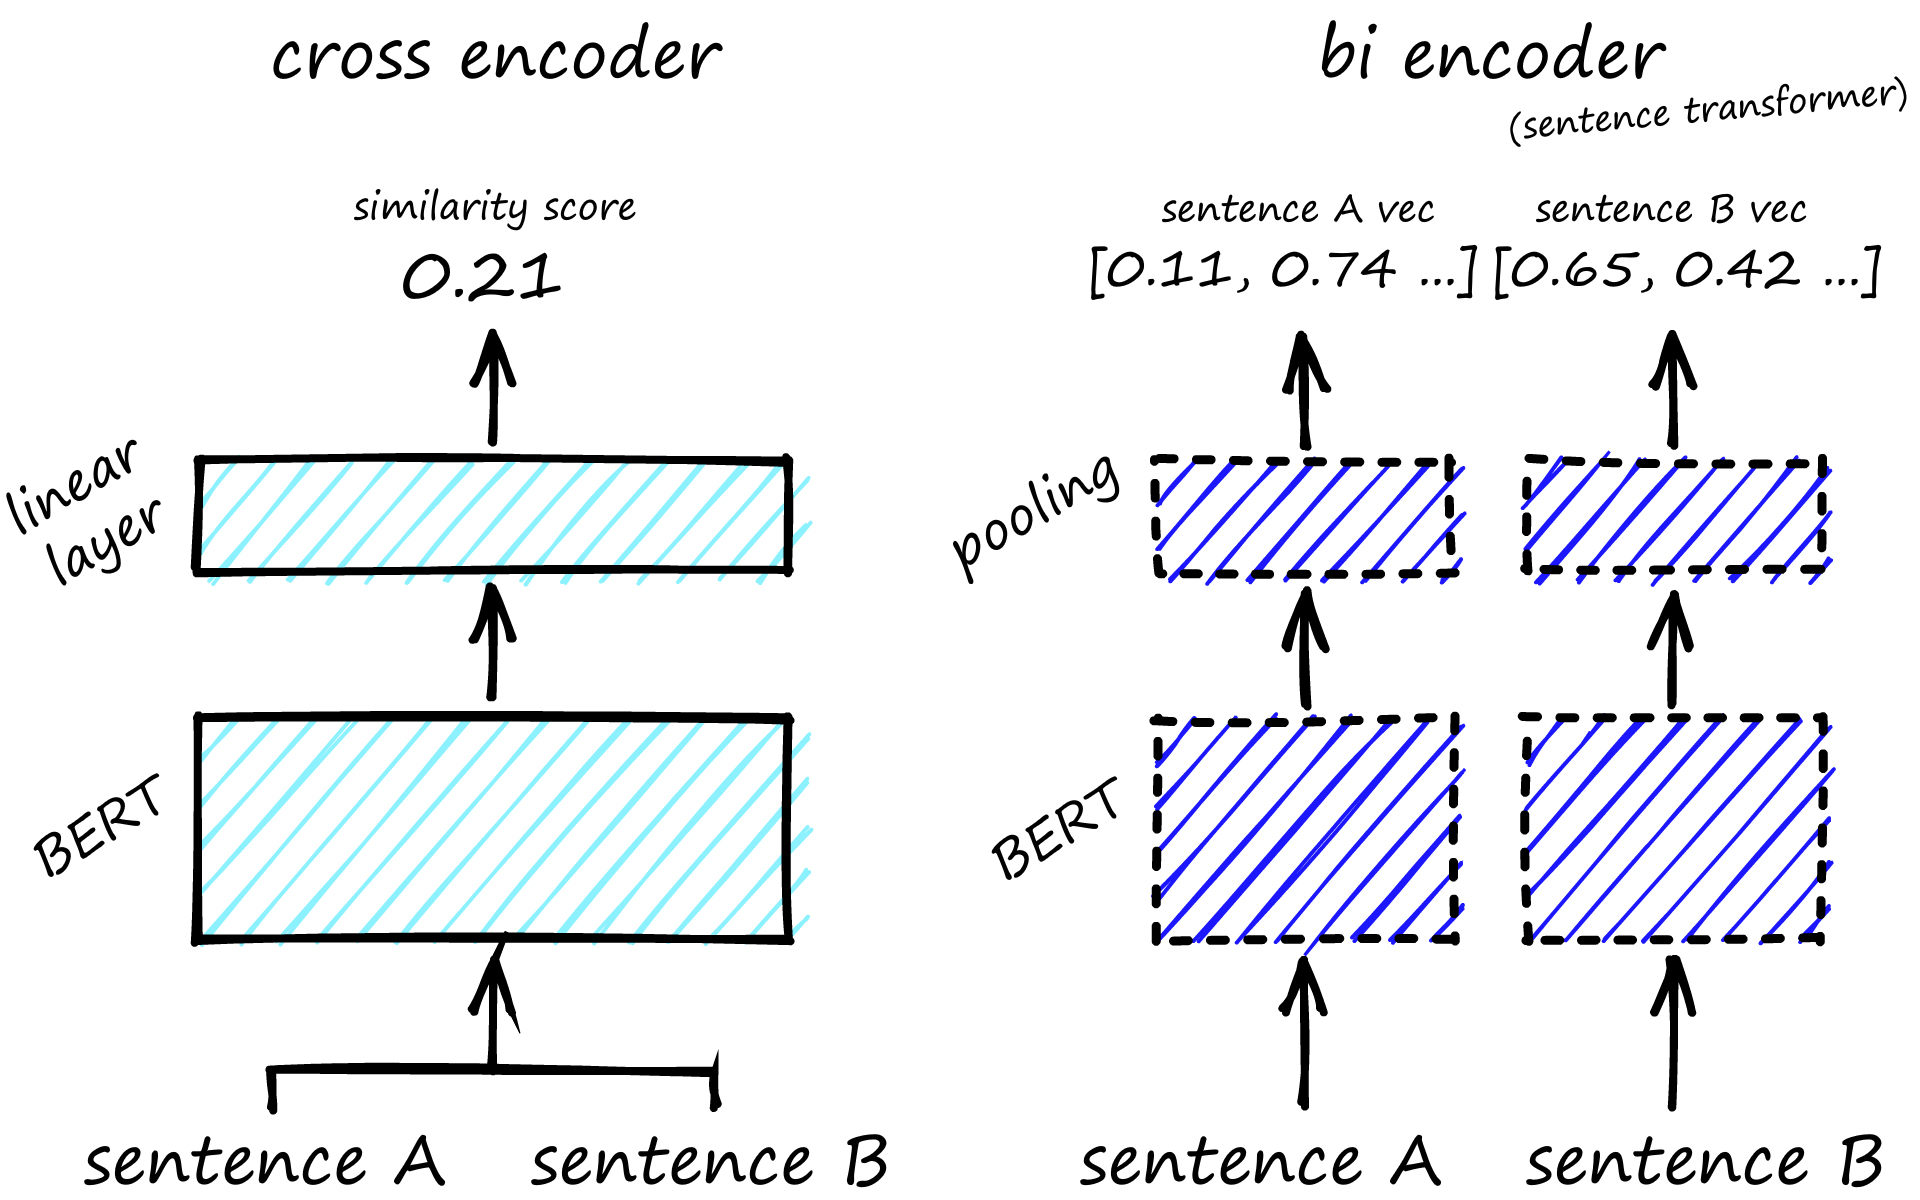
\includegraphics[width=12cm]{./assets/images/sbert1.jpg}
    \captionof{figure}{Sự khác biệt giữa cách tiếp cận của mô hình BERT và SBERT trong bài toán so sánh sự tương đồng ngữ nghĩa}
\end{minipage}

SBERT thêm vào một tầng pooling cho tầng output của BERT để lấy ra được
một embedding vector size cố định cho câu đó. Đã thử nghiệm trên cả 3 cách pooling và chọn phương thức MEAN Pooling:

\begin{itemize}
    \item[--] Sử dụng output của CLS token.
    \item[--] Sử dụng MEAN pooling.
    \item[--] Sử dụng MAX pooling.
\end{itemize}

\subsubsection{Finetune từ BERT, RoBERTa}

Và để fine-tune lại các mô hình BERT và RoBERTa, SBERT sử dụng kiến trúc siamese và triplet network.
Trong quá trình fine-tuning sẽ cập nhật trọng số sao cho các vector embedding đầu ra có ngữ nghĩa và có thể được so sánh bằng cosine similarity.

    \begin{minipage}
        {14cm}
        \captionsetup{type=figure}
        \centering
        \includegraphics[width=6cm]{./assets/images/sbert-softmax.png}
        \captionof{figure}{SBERT fine-tuned lại BERT sử dụng hàm đánh giá là Softmax Classifier (1)}
        \label{fig:demo-register-1}
    \end{minipage}

    \begin{minipage}
        {14cm}
        \captionsetup{type=figure}
        \centering
        \includegraphics[width=6cm]{./assets/images/sbert-cosine.png}
        \captionof{figure}{SBERT fine-tuned lại BERT sử dụng hàm đánh giá là Cosine Similarity (2)}
        \label{fig:demo-register-2}
    \end{minipage}

Trong quá trình fine-tuning, SBERT đã thử nghiệm với 2 hàm đánh giá khác nhau là Softmax Classifier và Cosine Similarity:

\begin{itemize}
    \item[--] Classification: \begin{itemize}
            \item[+] Nối embedding của u, v và phép tính element-wise |u - v|.
            \item[+] Nhân với trọng số  \(W_t \in \mathbb{R}^{3n \times k}\), và cho kết quả đi qua hàm softmax:
                \begin{equation}
                    o = \text{softmax}(W_t(u, v, |u - v|))
                \end{equation}
        \end{itemize}
    \item[--] Regression: Sử dụng cosine similarity để tính độ tương đồng giữa u và v, Sau đó dùng hàm loss là MSE (Mean Square Error) để tính độ lỗi.
\end{itemize}

Huấn luyện SBERT được diễn ra trên sự kết hợp của các tập dữ liệu SNLI \cite{snli:emnlp2015} (Bowman et al., 2015) và Multi-Genre NLI \cite{N18-1101} (Williams et al., 2018).
SNLI là một bộ sưu tập gồm \textbf{570,000} cặp câu được chú thích với các nhãn "contradiction" (mâu thuẫn), "entailment" (hỗ trợ), và "neutral" (trung lập).
MultiNLI chứa \textbf{430,000} cặp câu và bao gồm nhiều thể loại văn bản nói và viết khác nhau. Tinh chỉnh SBERT với một hàm mục tiêu là \textbf{Classification Softmax 3 chiều} trong một epoch. Sử dụng \textbf{batch size là 16}, tối ưu hóa Adam với tốc độ học \textbf{2e-5},
và tăng tốc tốc độ học tuyến tính trên 10\% dữ liệu huấn luyện. Chiến lược pooling sử dụng là \textbf{"MEAN"} (trung bình).


\subsection{Phương pháp RAG}
\subsubsection{Thực trạng của các mô hình ngôn ngữ}
Với sự phát triển bùng nổ của các mô hình ngôn ngữ lớn hiện nay đã mở đường cho những tiến bộ vượt bậc trong lĩnh vực xử lý ngôn ngữ tự nhiên cũng như đẩy mạnh việc ứng dụng AI tạo sinh vào cuộc sống

Tuy nhiên, những mô hình mạnh mẽ này cũng đi kèm với một số thách thức cần phải giải quyết.
Một trong những vấn đề lớn là hiện tượng "hallucination" - ảo giác, tức việc \ac{llm} tạo ra các thông tin không chính xác,
không đúng sự thật hoặc không được hỗ trợ bởi dữ liệu có sẵn. Hiện tượng này rất nguy hiểm bởi nó có thể dẫn đến việc cung cấp các thông tin sai lệch gây hậu quả nghiêm trọng và làm giảm độ tin cậy của các hệ thống dựa trên AI

\begin{minipage}{\linewidth}
    \centering
    \includegraphics[width=14cm]{./assets/images/hallucination.png}
    \captionsetup{type=figure}
    \caption{Định nghĩa về vấn đề "hallucination" ở LLMs.}
\end{minipage}

Hallucination \cite{huang2023survey} theo bài báo "\textit{A Survey on Hallucination in Large Language Models:
Principles, Taxonomy, Challenges, and Open Questions}" sẽ chia làm 2 loại: Ảo giác sự thật (Factuality Hallucination)
và Ảo giác tính trung thực (Faithfulness Hallucination).

Ảo giác sự thật (Factuality Hallucination) thể hiện khi thông tin cung cấp từ LLM có sự sai lệch
so với thông tin đã được xác nhận trong thế giới thực, những thông tin
này được coi như là một sự không nhất quán với sự thật hoặc là sự ngụy tạo do mô hình ngôn ngữ.

Còn với ảo giác tính trung thực (Faithfullness Hallucination) đề cập đến sự chệch lệch của nội dung được tạo ra so với 
hướng dẫn của người dùng hoặc bối cảnh được cung cấp bởi đầu vào, cũng như tính nhất quán trong nội dung được tạo ra.

Ví dụ, như trong Hình 2.12(a) thể hiện ảo giác sự thật (Factuality Hallucination), khi được hỏi về người đầu tiên đi bộ trên mặt trăng, mô hình có thể khẳng định rằng đó là Charles Lindbergh vào năm 1951.
Trong khi sự thật là Neil Armstrong là người đầu tiên đi bộ trên mặt trăng vào năm 1969 trong chuyến bay Apollo 11. 

Ngược lại, như minh họa trong Hình 1(b) thể hiện ảo giác tính trung thực (Faithfullness Hallucination), khi được yêu cầu tóm tắt một bài báo, mô hình đã không chính xác về ngày diễn ra xung đột giữa Israel và Hamas từ tháng 10 năm 2023 thành tháng 10 năm 2006. 

Một vấn đề khác với các \ac{llm}, chính là kiến thức bị lỗi thời. Ví dụ như dữ liệu đào tạo của ChatGPT 3.5 bị đóng băng ở thời điểm tháng 1/2022. 
Nếu hỏi ChatGPT về một sự kiện gì đó vào 2023, tình hình thời tiết, chính sách mới, vv. thì nó sẽ không trả lời được một thông tin chính xác.

\begin{minipage}{\linewidth}
    \centering
    \includegraphics[width=14cm]{./assets/images/llm-limitation-1.png}
    \captionsetup{type=figure}
    \caption{Đặt một câu hỏi nằm ngoài thời gian kiến thức huấn luyện của ChatGPT 3.5.}
\end{minipage}

\vspace{0.2cm}

Ngoài ra, các LLM được huấn luyện cho các nhiệm vụ tổng quát, (generalized tasks), nghĩa là nó sẽ không biết dữ liệu riêng tư của cá nhân hay tổ chức nào đó, 
cũng như thiếu các kiến thức ngành chuyên sâu hoặc thông tin về một đối tượng rất cụ thể nào đó (ví dụ sản phẩm mới ABC của một công ty XYZ). 

Một hạn chế khác cũng vô cùng quan trọng, chính là việc các LLM hoạt động như một hộp đen: 
nghĩa là không thể biết được LLM đã sử dụng những nguồn thông tin nào để đưa ra được câu trả lời. Điều này sẽ gây ra
khó khăn trong việc quản lý kiến thức của LLM, hạn chế những nguồn thông tin sai lệch hoặc không phù hợp.


\subsubsection{Định Nghĩa}
Phương pháp \ac{rag} là một phương pháp kết hợp giữa phương pháp truy vấn kết hợp và phương pháp sinh câu trả lời.
Phương pháp RAG \cite{lewis2021retrievalaugmented} này được giới thiệu lần đầu bởi các nhà nghiên cứu của Meta AI để giải quyết các nhiệm vụ yêu cầu nhiều kiến thức.
Nó là thành phần kết hợp giữa thành phần truy xuất thông tin (Retrieval) và một mô hình tạo sinh văn bản (Generation).

Trong quá trình hoạt động, một hệ thống RAG thường sử dụng một bộ truy xuất thông tin (retriever) để lấy các ngữ cảnh (context) liên quan đến câu hỏi hoặc yêu cầu của người dùng từ nguồn dữ liệu ngoại vi, chẳng hạn như một tập hợp các văn bản hoặc trang web. Sau đó, thông tin này được sử dụng như một phần của đầu vào cho một mô hình sinh tự nhiên như GPT để tạo ra câu trả lời hoặc văn bản mới.

\begin{minipage}{\linewidth}
    \centering
    \includegraphics[width=14cm]{./assets/images/RAG-procedure.jpg}
    \captionsetup{type=figure}
    \caption{Quá trình thực hiện phương pháp \ac{rag}.}
\end{minipage}

\vspace{0.2cm}

Phương pháp \ac{rag} ra đời để giải quyết cho việc ảo giác (hallucination) của các
mô hình ngôn ngữ lớn. Ý tưởng của phương pháp chính là kết hợp một phương pháp truy vấn
để tìm ra được các ngữ cảnh (context) có liên quan cho câu hỏi của người dùng. Sau đó sử dụng chính 
ngữ cảnh này để yêu cầu (prompt) cho các mô hình ngôn ngữ lớn mạnh mẽ như GPT, Llama2, Gemini,\dots

Bằng cách này, phương pháp RAG có thể giải quyết được một số hạn chế của LLM. Đầu tiên, nó đã giúp cho
LLM có được những kiến thức mới hoặc những tri thức chuyên sâu về một tác vụ cụ thể nào đó. Những kiến thức có thể đã không được
sử dụng để huấn luyện cho LLM đó.

Kế tiếp, phương pháp RAG này giúp kiểm soát được những thông tin mà LLM sẽ trả lời, biết được nguồn thông tin mà mô
hình ngôn ngữ sẽ sử dụng để sinh từ. Nhờ đó, hệ thống sẽ có được khả năng kiểm soát cao hơn với câu trả lời được sinh ra
từ các LLM.

\begin{minipage}{\linewidth}
    \centering
    \includegraphics[width=.8\linewidth]{./assets/images/RAG-evolution.png}
    \captionsetup{type=figure}
    \caption{Sự phát triển và xu hướng của kỹ thụât \ac{rag}.}
\end{minipage}

\vspace{0.5cm}

Áp dụng \acl{rag}, ta sẽ giải quyết được nhiều bài toán trên tập dữ liệu riêng tư hoặc tập dữ liệu chuyên môn, mà không cần huấn luyện hay finetune lại mô hình trên một tập dữ liệu cho tác vụ này.
Phương pháp RAG sẽ giúp có được sự kiểm soát cao hơn đối với mô hình, khi mà kiến thức của chúng dựa trên những thông tin được truyền vào prompt.

\subsubsection{Phân đoạn dữ liệu (chunking)}

Bước đầu tiên trong việc xây dựng một hệ thống hỏi đáp dựa trên phương pháp RAG chính là việc tiền xử lý và phân đoạn (dữ liệu):

\begin{minipage}{\linewidth}
    \centering
    \includegraphics[width=.8\linewidth]{./assets/images/RAG-simple.png}
    \captionsetup{type=figure}
    \caption{Tiền xử lý và phân đoạn dữ liệu trong hệ thống sử dụng \ac{rag}.}
    \label{fig:rag-simple}
\end{minipage}

\vspace{0.5cm}

Như ảnh \ref{fig:rag-simple} minh họa, bước phân đoạn dữ liệu hay chunking sẽ được thực hiện sau khi tập dữ liệu thô, không cấu trúc của chúng ta đã được tiền xử lý về dạng văn bản.
Tập dữ liệu thô này tốt nhất cũng cần phải được trích xuất thông tin cốt lõi, loại bỏ những thông tin nhiễu và không liên quan để hỗ trợ cho quá trình Chunking và khâu Retrieval nói chung.

Phân đoạn dữ liệu hay chunking chính là quá trình phân tách các văn bản thông tin của hệ thống hỏi đáp thành các đoạn thông tin nhỏ hơn.
Các chunk thông tin cần phải đảm bảo:

\begin{itemize}
    \item \textbf{Đủ thông tin:} Mỗi chunk thông tin cần chứa đủ thông tin để trả lời cho một câu hỏi hoặc một yêu cầu của người dùng.
    \item \textbf{Độ dài phù hợp} Các chunk thông tin cần chứa đủ thông tin và đồng thời cũng cần có một ngưỡng giới hạn độ dài. Vì các chunk thông tin sẽ 
    được sử dụng như là ngữ cảnh cho mô hình sinh câu trả lời, nên cần phải có độ dài phù hợp với context window của mô hình
    \item \textbf{Không trùng lặp:} Các chunk thông tin không được chứa thông tin trùng lặp với các chunk khác.
    \item \textbf{Dễ hiểu:} Các chunk thông tin cần phải dễ hiểu, dễ đọc, ý nghĩa rõ ràng có thể dễ tìm kiếm.
\end{itemize}

Mục tiêu của việc chunking thông tin là để cắt thông tin ra thành các phần nhỏ và mang ý nghĩa để có thể lưu và truy vấn một cách hiệu quả.
Việc này giúp cho bộ phận truy xuất thông tin (retriever) có thể tìm kiếm thông tin một cách nhanh chóng và chính xác hơn dựa vào câu hỏi được đặt ra. Với việc đưa một số chunk thông tin nhỏ và cho \ac{llm}
chi phí sẽ được giảm đáng kể thay vì phải đưa cả văn bản vào.

\begin{minipage}{\linewidth}
    \centering
    \includegraphics[width=.8\linewidth]{./assets/images/chunking-blog-post.png}
    \captionsetup{type=figure}
    \caption{Một ví dụ về chunking một bài viết trong hệ thống sử dụng \ac{rag}.}
    \label{fig:rag-blog-post}
\end{minipage}

\vspace{0.5cm}

Về cách để phân đoạn hay chunking dữ liệu, ta sẽ có một số cách tiếp cận và chiến thuật khác nhau.
Tùy theo yêu cầu của dữ liệu và bài toán, ta sẽ chọn chiến thuật chunking phù hợp và tối ưu nhất.

\textbf{Recursive Character Chunking}

Ý tưởng chính của phương pháp này là phân đoạn dữ liệu dựa trên các ký tự (character) của văn bản. Dựa vào số chunk size đặt trước, các 
chunk sẽ được phân tách sao cho mỗi chunk sẽ chứa một số ký tự nhất định. Tuy nhiên, ngoài tham số chunk size được quyết định trước, cũng có một vài
điều kiện khi phân tách chunk ở cách thức này. Chẳng hạn như không ngắt ngang một từ, mỗi chunk phải đảm bảo một độ dài tối thiểu nào đó.

Với chunk size = 100, ta sẽ phân đoạn một văn bản thành các chunk như sau:

\begin{minipage}{\linewidth}
    \centering
    \includegraphics[width=\linewidth]{./assets/images/recursive-chunkchunk.png}
    \captionsetup{type=figure}
    \caption{Một ví dụ cho Recursive Character Chunking.}
\end{minipage}

\vspace{0.5cm}

\textbf{Document Specific Chunking}

Với cách phân đoạn Document Specific Chunking, mục tiêu của cách tiếp cận là giữ nguyên và phân đoạn văn bản theo cấu trúc của văn bản đó.
Vì vậy, cách tiếp cận này không yêu cầu định nghĩa trước kích thước mỗi chunk, mà nó sẽ dựa vào cấu trúc của văn bản để tiến hành.
Cách tiếp cận này sẽ cố gắng giữ ý nghĩa cấu trúc văn bản của tác giả văn bản, nhờ vậy các chunk sẽ được đúng và đủ ý.

\begin{minipage}{\linewidth}
    \centering
    \includegraphics[width=\linewidth]{./assets/images/doc-specific-chunk.png}
    \captionsetup{type=figure}
    \caption{Một ví dụ cho Document Specific Chunking.}
\end{minipage}

\vspace{0.5cm}

\textbf{Token-based Chunking}

Mỗi mô hình ngôn ngữ đều có một tokenizer với kích thước là cố định và đầu vào không nên vượt quá giới hạn đó. Mục tiêu của phương pháp chunking
này. Cách chunking này sẽ có nguyên lý hoạt động giống với Recursive Character Chunking, tuy nhiên nó được bổ sung thêm điều kiện để đảm bảo độ dài phù hợp
cho mô hình ngôn ngữ đang sử dụng.

\vspace{0.5cm}

\begin{minipage}{\linewidth}
    \centering
    \includegraphics[width=\linewidth]{./assets/images/token-chunking.png}
    \captionsetup{type=figure}
    \caption{Một ví dụ cho Token-based Chunking.}
\end{minipage}

\vspace{0.5cm}

\subsubsection{Truy vấn thông tin ở bộ Retriever}

Thông tin sau khi đã được phân đoạn sẽ được lưu trữ và quản lý trong bộ truy xuất thông tin (retriever).
Để lưu trữ được các chunk thông tin, ta cần sử dụng một mô hình Bi-encoder để nhúng văn bản thành một dạng vector số như sau:


\vspace{0.5cm}

\begin{minipage}{\linewidth}
    \centering
    \includegraphics[width=.7\linewidth]{./assets/images/bi-encoder.png}
    \captionsetup{type=figure}
    \caption{Nhúng văn bản với Bi-encoder.}
\end{minipage}

\vspace{0.5cm}

Tùy thuộc vào kiến trúc của mô hình, ta sẽ thu được một vector ngữ nghĩa đặc với một số chiều cố định.
Với mô hình Vietnamese SBERT, số chiều của vector đầu ra sẽ là \(d_{\text{SBERT}} = 768\).
Những vector này đại diện cho ngữ nghĩa của các chunk thông tin và sẽ được sử dụng để tìm kiếm thông tin phù hợp với câu hỏi của người dùng.

Với các mô hình Bi-encoders này, kiến trúc của nó sẽ bao gồm một tầng BERT để nhúng văn bản và một tầng Pooling để lấy ra được một vector nhúng với chiều dài cố định.
Cụ thể khi nhận đầu vào là một chuỗi văn bản, mô hình sẽ hoạt động như sau:

\vspace{0.5cm}

\begin{minipage}{\linewidth}
    \centering
    \includegraphics[width=\linewidth]{./assets/images/bi-encoder-io.png}
    \captionsetup{type=figure}
    \caption{Đầu vào và đầu ra của các mô hình Bi-encoder.}
    \label{fig:bi-encoder-io}
\end{minipage}

\vspace{0.5cm}

Như ảnh \ref{fig:bi-encoder-io} đã ví dụ, khi nhận đầu vào là một câu \textit{"my dog is fast"}, tầng BERT sẽ tạo ra một ma trận embedding có kích thước là 4 x 768 (trong phiên bản BERT base), hoặc 4 x 1024 (trong phiên bản BERT large). Sau đó biểu diễn ngữ nghĩa sẽ được đưa qua tầng Pooling để tạo thành một vector đặc với số chiều cố định.

Hai vector này sẽ được lưu lại và có thể so sánh sự tương đồng bằng hàm cosine similarity. Nhờ đó ta có được một cách để truy vấn nhanh
các văn bản tương đồng với nhau trong hệ thống.

\vspace{0.5cm}

\begin{minipage}{\linewidth}
    \centering
    \includegraphics[width=\linewidth]{./assets/images/rag-embedding.png}
    \captionsetup{type=figure}
    \caption{Quá trình nhúng văn bản trong bộ phận retrieval.}
\end{minipage}

\vspace{0.5cm}

Với hệ thống RAG, khi nhận được câu hỏi từ user, đầu tiên hệ thống sẽ nhúng câu hỏi này thành dạng vector đặc
với cùng mô hình Bi-encoder khi nhúng các chunk thông tin. Sau khi có được vector này, hệ thống RAG sẽ so sánh sự tương đồng giữa vector câu hỏi và các vector chunk thông tin nhằm chọn 
ra \textit{top k} chunk thông tin liên quan nhất với câu hỏi của người dùng.

Ở đây, việc lựa chọn k là một tham số quan trọng, nó sẽ ảnh hưởng đến việc trả lời của hệ thống. 
Nếu k quá nhỏ, hệ thống sẽ không thể trả lời được câu hỏi của người dùng, ngược lại nếu k quá lớn, hệ thống sẽ trả về quá nhiều thông tin không cần thiết gây loãng thông tin hoặc không fit với context window của mô hình sinh.

\begin{minipage}{\linewidth}
    \centering
    \includegraphics[width=\linewidth]{./assets/images/vectordb.png}
    \captionsetup{type=figure}
    \caption{Cơ sở dữ liệu vector.}
\end{minipage}

Những vector này sẽ được lưu trữ trong một \textit{cơ sở dữ liệu vector}. Như ý nghĩa của tên, đây là một loại cơ sở dữ liệu chứa các loại embedding hoặc vector cho nhiều loại dữ liệu khác nhau
như hình ảnh, văn bản, video, âm thanh, \dots Cơ sở dữ liệu Vector cung cấp khả năng tạo truy vấn vector nhanh với một số 
hàm so sánh như cosine similarity, euclidean distance.

Như vậy trong hệ thống RAG và bài toán hỏi đáp, cơ sở dữ liệu vector là nơi lưu trữ các vector embedding của các chunk thông tin.
Nếu xem mô hình ngôn ngữ lớn là bộ não của hệ thống RAG, thì cơ sở dữ liệu vector có thể xem như thành phần quản lý kiến thức của mô hình.
Nó quyết định những kiến thức nào sẽ được sử dụng để sinh câu trả lời cho câu hỏi của người dùng.
    

\subsubsection{Tạo sinh câu trả lời với LLM và context}

Sau khi đã có được các chunk thông tin liên quan nhất với câu hỏi của người dùng, hệ thống sẽ sử dụng các chunk thông tin này như là ngữ cảnh (context) cho mô hình sinh câu trả lời.

Lúc này đầu vào của mô hình ngôn ngữ sẽ bao gồm prompt, câu hỏi của người dùng và context. Tất cả đều được concatenate và đưa vào mô hình sinh câu trả lời.
Với mỗi mô hình ngôn ngữ, ta nên áp dụng các prompt template phù hợp và giống với cấu trúc dữ liệu huấn luyện của mô hình đó. Xét một ví dụ về prompt template cho mô hình \textit{PhoGPT}:

\begin{center}
    \textit{"\#\#\# Câu hỏi: {Đăng ký giấy khai sinh cho con cần chuẩn bị những thủ tục gì} \\ \#\#\# Trả lời:"}
\end{center}



\subsection{Xếp hạng lại trong RAG (Re-ranking)}

\subsubsection{Vấn đề với RAG thông thường}
Với các hệ thống sử dụng RAG, chúng ta cần thực hiện việc tìm kiếm ngữ nghĩa qua nhiều tài liệu văn bản.
Con số này có thể  tăng lên đến hàng chục nghìn đến hàng triệu văn bản với những hệ thống có quy mô lớn và tập dữ liệu thô rộng.

Để đảm bảo được hiệu năng và thời gian xử lý cho các hệ thống ở quy mô này, ta bắt buộc phải sử dụng tìm kiếm bằng vector
nhằm đảm bảo thời gian tìm kiếm nhanh, khả thi trong thực tế.

Tuy nhiên, việc tìm kiếm bằng vector cũng không tránh khỏi những vấn đề. Với các chunk thông tin văn bản,
việc nén ngữ nghĩa của chúng chỉ thành một vector đặc với size cố định - thông thường có chiều là 768 hoặc 1536 sẽ dẫn đến việc mất mát thông tin.
Điều này là gần như không thể tránh khỏi, đặc biệt là với các chunk thông tin có ý nghĩa phức tạp và chi tiết.

Do việc mất mát thông tin này, các chunk thông tin truy vấn được bằng top k vector search sẽ không phải luôn chính xác và có thể tin cậy được.
Một số chunk thông tin mặc dù được xếp hạng thấp hơn top k lại chứa nhiều thông tin hơn và chính xác hơn.
Cách dễ nhất cho vấn đề này chính là tăng số k lên, truyền nhiều chunk hơn làm context cho \ac{llm}.

Tuy nhiên, mỗi mô hình ngôn ngữ để có một context window, biểu thị số lượng token tối đa mà mô hình có thể xử lý một lúc. Do đó, không thể truyền vào quá nhiều chunk thông tin cho LLM.
Ngoài ra quá nhiều thông tin được truyền vào sẽ gây loãng và tình trạng \textit{"Lost in the middle"} cho mô hình ngôn ngữ.

\begin{minipage}{\linewidth}
    \centering
    \includegraphics[width=.7\linewidth]{./assets/images/lost-middle.png}
    \captionsetup{type=figure}
    \caption{Vấn đề Lost in the Middle với các LLM.}
\end{minipage}

Ta sẽ sử dụng metric là \textit{recall@k} để đánh giá hiệu suất của hệ thống tìm kiếm thông tin. Metric này sẽ đo lường xem trong top k chunk thông tin trả về, có bao nhiêu chunk thông tin chứa thông tin chính xác và đầy đủ cho câu hỏi của người dùng.

\begin{equation}
    \text{recall@k} = \frac{\text{Các chunk thông tin có liên quan trong top k}}{\text{Tổng chunk thông tin có liên quan}}
\end{equation}

Để cải thiện metric này, ta cần nghĩ đến việc lấy được thật nhiều chunk thông tin (tăng số k) và chỉ giữ lại
những chunk thông tin chứa thông tin chính xác và đầy đủ nhất cho LLM. Điều này chính là mục tiêu của việc xếp hạng lại trong RAG. 

\subsubsection{Phương pháp Re-ranking}
Phương pháp Re-ranking sẽ làm điều này bằng cách sử dụng một mô hình Cross Encoder gọi là Re-ranker để xếp hạng lại các chunk thông tin đã được truy xuất từ bộ retriever:

\begin{minipage}{\linewidth}
    \centering
    \includegraphics[width=.9\linewidth]{./assets/images/reranking.png}
    \captionsetup{type=figure}
    \caption{Phương pháp Re-ranking trong RAG.}
\end{minipage}
\vspace{0.5cm}

Bước reranking sẽ được thực hiện sau khi đã hoàn thành retrieval và trước khi truyền vào mô hình sinh câu trả lời. Ở bộ phận retrieval
, ta sẽ cho phép chọn một số k chunk lớn hơn (ví dụ k=25 như trong ảnh). Sau đó ở bước re-ranking này, ta sẽ dùng mô hình re-ranker để lọc lại một vài chunk thông tin liên quan nhất.

Sở dĩ, mô hình re-ranker có được khả năng so sánh độ tương đồng chính xác hơn là vì nó sử dụng mô hình Cross Encoder chứ không phải Bi Encoder sử dụng ở vector search.
Với khả năng cho phép hai câu văn bản A và B cùng đi vào một lúc để so sánh mà không cần nén thành vector biểu diễn như ở Bi Encoder, độ chính xác của Cross Encoder sẽ tốt hơn.
Tuy nhiên nó cũng có sự đánh đổi đó chính là thời gian xử lý, vì vậy hệ thống RAG thường tận dụng ưu điểm của cả hai kiến trúc mô hình này bằng cách xây dựng hệ thống RAG \textit{"Two-Stage Retrieval with Reranking"}

\begin{minipage}{\linewidth}
    \centering
    \includegraphics[width=.9\linewidth]{./assets/images/2phaseRAG.png}
    \captionsetup{type=figure}
    \caption{Hệ thống RAG Two-Stage Retrieval with Reranking.}
\end{minipage}
\vspace{0.5cm}

Bằng cách này, ta tận dụng sự nhanh và khả năng mở rộng của Bi Encoder cho phase tìm kiếm đầu tiên và tận dụng được sự chính xác của Cross Encoder ở bước re-ranking.

\subsection{Truy vấn kết hợp trong RAG (RAG Fusion)}
% # TODO: Truy vấn kết hợp trong RAG (RAG Fusion)

\subsection{Đánh giá kết quả từ phương pháp RAG}
% # TODO: Đánh giá kết quả từ phương pháp RAG

\section{Phương pháp thực hiện}
Trong chương này, đầu tiên, luận văn sẽ trình bày chi tiết phương pháp ứng dụng RAG vào trong hệ thống tư vấn thủ tục hành chính. Hệ thống sử dụng
mô hình SBERT để nhúng văn bản và mô hình ngôn ngữ lớn GPT-3.5 để sinh câu trả lời. Với đầu vào là một câu hỏi của người dùng, 
hệ thống cần trả về một câu trả lời giải quyết được vấn đề của người dùng đi kèm với các trích dẫn thông tin về thủ tục hành chính phù hợp tại Cần Thơ.

Tiếp theo, ở chương này sẽ trình bày từng bước phương pháp xây dựng hệ thống theo kiến trúc Microservices.
Hệ thống cần đảm bảo khả năng mở rộng, cô lập các tính năng và khả năng chịu lỗi cao.

Các bước thực hiện cho hệ thống sẽ được trình bày dựa vào 2 sơ đồ sau:
\subsection{Thu thập dữ liệu}
\subsubsection{Mô tả dữ liệu}
Dữ liệu được sử dụng cho phương pháp RAG - cũng là dữ liệu hệ thống dựa vào để có thể sinh câu trả lời cho câu hỏi họăc tình huống
của người dùng chính là các thủ tục hành chính tại Cần Thơ.

Tất cả các trường dữ liệu thông tin của một thủ tục hành chính đều ở dạng chuỗi. Một thủ tục hành chính bao gồm các thông tin như tên, lĩnh vực, trình tự thực hiện,
cách thức thực hiện, thành phần hồ sơ, căn cứ pháp lý, ... Dữ liệu của một thủ tục hành chính có thể được tìm thấy ở phần phụ lục.

\vspace{0.5cm}
\begin{minipage}{14cm}
    \begin{center}
        \begin{tabular}{ | m{3cm} | m{11cm}| } 
        \cline{1-2} 
        \hline
        \textbf{Trường} & \textbf{Thông tin}\\
        \hline Mã thủ tục & 1.004269.000.00.00.H13 \\
        \hline Tên & Thủ tục cung cấp dữ liệu đất đai (cấp tỉnh) \\
        \hline Trình tự thực hiện & 
                Bước 1:
                - Tổ chức, cá nhân có nhu cầu khai thác dữ liệu đất đai nộp phiếu yêu cầu hoặc gửi văn bản yêu cầu đến Trung tâm Dữ liệu và Thông tin đất đai thuộc Tổng cục Quản lý đất đai hoặc Văn phòng đăng ký đất đai. Đối với địa phương chưa xây dựng cơ sở dữ liệu đất đai, Văn phòng đăng ký đất đai, Ủy ban nhân dân cấp xã;

                Bước 2:
                - Khi nhận được phiếu yêu cầu, văn bản yêu cầu hợp lệ của tổ chức, cá nhân, cơ quan cung cấp dữ liệu đất đai thực hiện việc cung cấp dữ liệu cho tổ chức, cá nhân có yêu cầu khai thác dữ liệu. Cơ quan cung cấp dữ liệu đất đai tiếp nhận, xử lý và thông báo nghĩa vụ tài chính (trường hợp phải thực hiện nghĩa vụ tài chính) cho tổ chức, cá nhân. Trường hợp từ chối cung cấp dữ liệu thì phải có văn bản trả lời nêu rõ lý do;
                
                \begin{center}
                    ...
                \end{center}
                \\
        \hline
        \end{tabular}
    \end{center}
    \captionsetup{type=table}
    \caption{Giới thiệu một thủ tục hành chính}
\end{minipage}

Nguồn dữ liệu sẽ được cào trực tiếp từ hệ thống thông tin giải quyết thủ tục hành chính thành phố Cần Thơ.
Với tổng cộng 1,827 thủ tục hành chính chia vào 99 nhóm dịch vụ công.
\subsubsection{Cào dữ liệu các thủ tục hành chính}
Dữ liệu các thủ tục hành chính sẽ được cào sử dụng thư viện Selenium với ngôn ngữ lập trình Python. Selenium là một thư viện hỗ trợ tự động hóa việc điều khiển trình duyệt web, 
bằng cách mở và điều khiển trình duyệt web bằng Selenium Webdriver.
Quá trình cào dữ liệu sẽ được thực hiện đa luồng, mỗi luồng sẽ điều khiển một trình duyệt web riêng biệt giúp tăng tốc độ cào dữ liệu.

Phương pháp cào dữ liệu sẽ được trình bày dựa vào sơ đồ bên dưới:

\begin{minipage}{\linewidth}
    \centering
    \includegraphics[width=14cm]{./assets/images/procedure-crawl.png}
    \captionsetup{type=figure}
    \caption{Sơ đồ quy trình cào dữ liệu các thủ tục hành chính.}
\end{minipage}

Đầu tiên, webdriver truy cập vào trang dịch vụ công của thành phố Cần Thơ. Tại đây, webdriver sẽ lấy danh sách các nhóm dịch vụ công ở mỗi trang.
Tiếp theo, chương trình chia làm 10 luồng để truy cập vào từng trang chi tiết của thủ tục hành chính, sử dụng thư viện BeautifulSoup để lấy dữ liệu, cấu trúc hóa và lưu vào các tệp file json tương ứng với mã thủ tục.

Trong quá trình thu thập dữ liệu, có một số trường hợp bị lỗi do cách thức hiển thị của trang web. Những trường hợp này sẽ được lưu lại trong tệp log để xử lý thủ công. Dữ liệu thu thập cuối cùng sẽ đầy đủ 1,827 thủ tục hành chính từ hệ thống thông tin giải quyết thủ tục hành chính thành phố Cần Thơ.
\subsection{Tiền xử lý dữ liệu}

Đối với phương pháp RAG, việc tiền xử lý dữ liệu là một bước quan trọng để hỗ trợ cho khâu truy vấn (Retrieval).
Để tiền xử lý dữ liệu cho hệ thống RAG hỗ trợ thủ tục hành chính Cần Thơ, các thao tác được thực hiện như ảnh sau:

\begin{minipage}{\linewidth}
    \centering
    \includegraphics[width=\linewidth]{./assets/images/preprocess.drawio.png}
    \captionsetup{type=figure}
    \caption{Sơ đồ chunking dữ liệu cho một thủ tục hành chính.}
\end{minipage}

Với mỗi thủ tục hành chính cào được, tách lần lượt thông tin thành các chunk nhỏ hơn, với kích thước của mỗi chunk 
là tương đương nhau. Ngoài ra, để giữ được ngữ cảnh cho thông tin (context), mỗi chunk sẽ được thêm một câu mô tả tùy thuộc vào thông tin nó chứa.
Với chunk thông tin chung của thủ tục hành chính \textit{Cấp phép hoạt động giáo dục kỹ năng sống và hoạt động giáo dục ngoài giờ chính khóa} như sau:

\vspace{0.5cm}
"\textit{Thủ tục hành chính tên Cấp phép hoạt động giáo dục kỹ năng sống và hoạt động giáo dục ngoài giờ chính khóa với mã 1.000181.000.00.00.H13 có các thông tin về  tên, số quyết định, cấp thực hiện, loại thủ tục và lĩnh vực như sau:}"

Mục đích của câu thông tin được chèn thêm này dùng đễ giữ lại ngữ cảnh cho chunk thông tin và hỗ trợ cho khâu truy vấn thông tin (retrieval phase) cho hệ thống RAG.
Điều quan trọng ở đây là khi truy vấn, hệ thống sẽ không tìm dựa vào cả đoạn thông tin, mà sẽ sử dụng câu
được chèn vào để tìm. Bên dưới là một ví dụ cho quá trình này:

\begin{minipage}{\linewidth}
    \centering
    \includegraphics[width=\linewidth]{./assets/images/search.drawio.png}
    \captionsetup{type=figure}
    \caption{Truy vấn thông tin sau khi đã tiền xử lý dữ liệu.}
\end{minipage}

\subsection{Xây dựng mô hình phân lớp ngữ cảnh dựa trên câu hỏi}
% # TODO: Xây dựng mô hình lọc ngữ cảnh phù hợp



\subsection{Xây dựng hệ thống ứng dụng phương pháp RAG}
% # TODO: Xây dựng hệ thống ứng dụng phương pháp RAG

\subsection{Đánh giá kết quả}
% # TODO: Đánh giá kết quả

\subsection{Triển khai hỗ trợ tư vấn thủ tục hành chính}
% # TODO: Triển khai hỗ trợ tư vấn thủ tục hành chính

\section{Kết quả thực nghiệm}
% # TODO: Kết quả thực nghiệm

\chapter{Kết luận}
\section{Kết quả đạt được}
% # TODO: Kết quả đạt được

\section{Hạn chế và hướng phát triển}
% # TODO: Hạn chế và hướng phát triển

\printbibliography

\chapter*{Phụ lục}
\addcontentsline{toc}{chapter}{Phụ lục}

\textbf{File json chứa thông tin một thủ tục hành chính}




\end{document}